\documentclass[conference]{IEEEtran}
\usepackage[utf8]{inputenc}
\IEEEoverridecommandlockouts
\usepackage{cite}
\usepackage{amsmath,amssymb,amsfonts}
\usepackage{graphicx}
\usepackage{caption}
\usepackage{subcaption}
\captionsetup{font=footnotesize}
\usepackage{float}
\usepackage{listings}
\usepackage{algorithmic}
\usepackage{graphicx}
\usepackage{textcomp}
\usepackage{xcolor}
\usepackage{booktabs}
\usepackage{hyperref}

\newcommand\tab[1][0.5cm]{\hspace*{#1}}
\def\BibTeX{{\rm B\kern-.05em{\sc i\kern-.025em b}\kern-.08em
    T\kern-.1667em\lower.7ex\hbox{E}\kern-.125emX}}
\begin{document}

\title{MONITORING SYSTEM FOR THE USE OF PERSONAL PROTECTIVE EQUIPMENT WITH THE APPLICATION OF DEEP LEARNING NETWORK}

\author{\IEEEauthorblockN{Son (Thai) Nguyen}
\IEEEauthorblockA{\textit{PFIEV 2015} \\
\textit{Ho Chi Minh University of Technology}\\
Ho Chi Minh city, Viet Nam\\
1512847@hcmut.edu.vn}
}

\maketitle
\begin{abstract}
The idea of artificial intelligence and computer vision working together for surveillance has been around for a long time. However, only came in recent years when the computing hardware can meet the technical and economic requirements for application purpose that the usage of these technologies gradually becomes popular. One of the applications that gained tremendous amount of attention is ensuring the safety of the construction workers. Through a supervisory system of cameras with artificial intelligence as a detector to monitor the use of personal protective equipment of site workers. In the context of this thesis, the system will focus on three common equipment at construction sites: hard hats, safety vest and face mask. The system uses YOLO, a CNN object detection algorithm. When operating, the system will be able to detect and categorize the use of personal protection equipment by workers at the construction site. If the system detects a case of non-use of personal protection equipment then the system will send alerts to the ones in charge of the site so that actions can be conducted before an irreversible accident happens. This will greatly improves the safety of working labors in construction site. The system is written in Python using YOLOv3 machine learning model and open source computer vision library OpenCV.

\textit{Keyword}—PPE detection . YOLOv3 . Surveillance
\end{abstract}

\section{Problems in labor safety supervision and artificial intelligence application solutions}
The construction industry has always been considered as one of the industries with high risks of occupational accidents and the possibility of occupational diseases. In fact, many serious accidents have happened, taking away lives or leaving serious injuries for workers, making them incapable of working and living as normal people. It is followed by emotional pain and economic burden for the family members of the victims. Therefore, ensuring occupational safety and health is always one of the top concerns at all levels and sectors. According to a report \cite{tnld:2019:gov} of 63/63 provinces and centrally run cities of Vietnam in 2019, \textbf{7130} labor accidents occurred with the total of \textbf{7267} victims. The statistics are shown in table \ref{table:tnld_stats}.
\begin{center}
  \begin{tabular} {l l}
  \toprule
  \midrule
  Number of deaths & 610 people\\
  \\
  Number of fatal labor accidents & 572 cases\\
  \\
  Number of seriously injured victims & 1592 people \\
  \\
  Number of female victims & 2535 people \\
  \\
  Number of labor accidents with two & 119 cases \\
  or more victims \\
  \bottomrule
  \end{tabular}
\end{center}
\captionof{table}{Data on labor accident situation in 2019.\label{table:tnld_stats}}

One of the main causes of tragic accidents is that workers do not use personal protective equipment during the work process. This issue not only stems from the subjectivity of the individual employee but also the shortcomings in the supervision of the works of the contractor and the employer. The table \ref{table:tnld_reason} shows the main causes of fatal occupational accidents in 2019.
\begin{center}

  \begin{tabular} {l l l}
  \toprule
  \it Cause & \it \% total no & \it \% total no \\
   & \it of cases & \it of deaths \\
  \midrule
  \textbf{Employers do not have a} \\ 
  \textbf{safe working processes} & \textbf{24.32} & \textbf{26.27} \\
  \textbf{and measures} \\
  \\
  \textbf{Employers do not provide} \\ 
  \textbf{occupational safety} \textbf{14.41} & \textbf{13.56} \\
  \textbf{and sanitation training} \\
  \textbf{for employees.} \\
f  \\
  \textbf{Due to labor organization} & \textbf{7.21} & \textbf{8.47} \\
  \textbf{and working conditions} \\
  \\
  \textbf{Equipment does not} & \textbf{1.8} & \textbf{1.69} \\
  \textbf{guarantee labor safety} \\
  \\
  \textbf{The employee violates} \\ 
  \textbf{the process of} & \textbf{14.41}  & \textbf{14.41} \\ 
  \textbf{occupational safety} \\
  \textbf{standard} \\
  \\
  \it {Other objective reasons,} & \it 37.85 & \it 35.6 \\
  \it {hard to avoid} \\
  \bottomrule
  \end{tabular}

\captionof{table}{The main causes of fatal accidents.
\label{table:tnld_reason}}
\end{center}

For workers, the harsh conditions of the work environment such as high outdoor temperatures or frequent vigorous physical activity causing the body to perspire constantly and many are willing to risk their safety in return for comfort. As for the building supervisors, they cannot cover the whole working process in different workplaces, so it is impossible to remind workers in time before the disaster happens whereas fatal consequences can be avoided or mitigated if workers use personal protective equipment.

In order to strengthen the implementation capacity to ensure labor safety in the works, many investors and contractors have installed camera systems to monitor work processes. These systems enable supervisors to observe multiple locations at the same time without having to move through different locations in the project, minimizing the cost and time of performing safety tasks. However, when the number of areas to be observed increased or the people in charge of observation did not focus on the task, monitoring through the monitor was likely to cause errors. The integration of AI technology into surveillance systems will increase the reliability of the safety work, minimize unnecessary errors. The objective of the paper is to develop and evaluate a system that identifies the use of personal protective equipment by workers at the construction site to assist supervisors in occupational safety assurance. The scope of the paper is to carry out detection on videos extracted from cameras. The detection model is trained using the built-in framework. The data set used to train and evaluate the identification model is collected and labeled by the author. Part of the image in this data set is derived from other data sets but does not reuse the labels of those data sets. The personal protective equipment which the system can detect include: hard hats, protective clothing and masks.

\section{Theoretical basis of artificial neuron network and YOLOv3 model}
\subsection{Artificial neural network}
Artificial neural networks are usually organized into layers. Figure \ref{fig:nn} shows the structure of a simple artificial neuron network. The first layer is the input layer used to get input data for neural networks. The last layer is the output layer, this layer will give the final calculation results of the classes that need to be predicted with the corresponding input data. The middle layers are called the hidden layers which each contains the neurons that have the activation functions and the weight links, these layers responsible for extracting the characteristics from the input signal and providing predictions. The learning process of an artificial neural network takes place in hidden layers. We can see that neurons in the same class are not connected to each other, but each neuron of the previous class will connect to all neurons of the next layer except bias. Therefore these layers are also called fully connected layers.
\begin{figure}[ht]
	\centerline{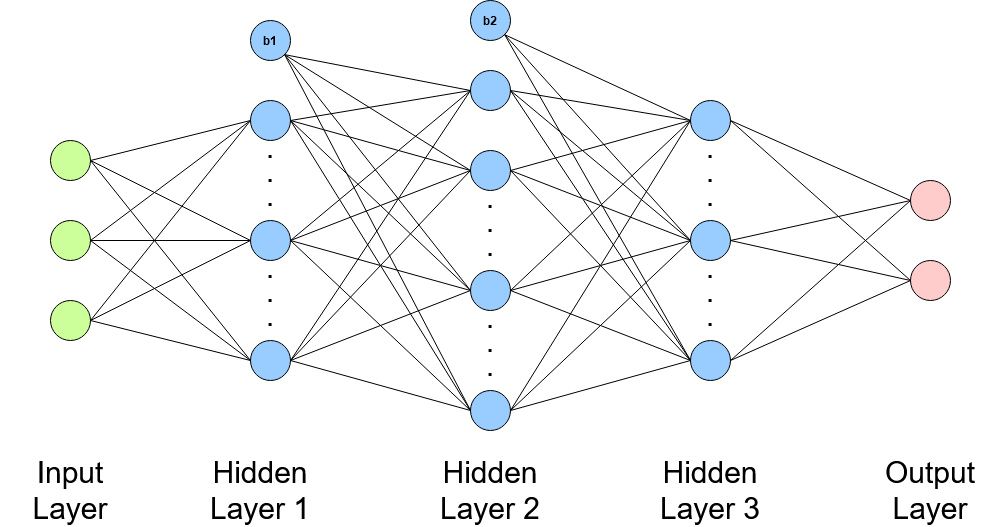
\includegraphics[scale=0.2]{images/nn.png}}
  	\caption{Simple neural network model with 3 hidden layers, 1 input layer and 1 output layer.}
  	\label{fig:nn}
\end{figure}
The process of artificial neural networks taking data from the input layer, pushing data through hidden layers and returning results at the output layer is called the \emph{feed-forward} process. Figure \ref{fig:ann} and the system of equation \ref{ann_eq} depict the general mathematical model of hidden layers during the feed-forward process of a neuron network.
\begin{figure}[ht]
	\centerline{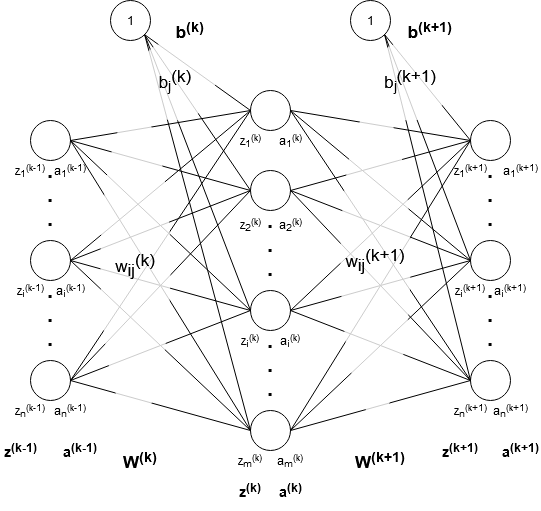
\includegraphics[scale=0.35]{images/ann.png}}
  	\caption{Mathematical model of the hidden layers of a artificial neural network.}
  	\label{fig:ann}
\end{figure}
\begin{align}
	a^{(0)}&=x \nonumber\\
	z^{(k)}&={\boldsymbol{W}^{(k)T}}{a^{(k-1)}}+{\boldsymbol{b}}^{(k)},k=1,2,..,N \label{ann_eq}\\
	a^{(k)}&=f^{(k)}\left(z^{(k)}\right),k=1,2,..,N \nonumber\\
	\widehat{y}&=a^{(N)} \nonumber
\end{align}
Where $\boldsymbol{W}^{(k)}$ is the weight matrix of the links between the $k-1$\emph{th} layer and the $k$\emph{th} layer, $\boldsymbol{b}^{(k)}$ is the bias vector of the $k$\emph{th} layer, $ z ^ {(k)} $ is the input vector of the hidden layer $ k $, $ a ^ {(k)} $ is the output vector of the hidden layer $ k $. During feed-forward, consider the $i$\emph{th} neuron of the $ (k-1) $\emph{th} layer with the output $ a ^ {(k-1)} _ i $, the input $ z ^ {(k)} _ j $ of the $ j $\emph{th} neuron in the $ k $\emph{th} layer is the sum of the outputs of the $ k-1 $\emph{th} layer neurons with weights $ w ^ {(k)} _ {ij} $ plus bias $ b ^ {(k)} _ {j} $. The equation that describes the process is $z^{(k)}_j={\sum_i} \left( {a^{(k-1)}_i} \times {w^{(k)}_{ij}} \right) + {{b}^{(k)}_j}$.

Then for each input value $ z ^ {(k)} _ i $ of a $ i $ neuron of the $ k $ class we will have a neuron output value of $ a ^ {(k)} _ i = f ^ {(k)} \left( z ^ {(k)} _ i \right) $ with $ f ^ {(k)} $ is the stimulus function of neurons in the $ k $\emph{th} layer. This process happens continuously between hidden layers in the neural network, so the output layer results in $ \widehat {y} = a ^ {(N)} $ with an input data $ a ^ {(0 )} = x $ depends on $ \boldsymbol {W} ^ {(k)} $ and $ \boldsymbol {b} ^ {(k)} $. Initially the weight matrices and bias vectors are randomly generated or according to a predetermined rule, but the predicted results of neural networks with these initial values will not be accurate. For human, in order to be able to master an operation, an individual need to undergo a learning process, the idea for learning of a neuron network is that for every input value, after the feed-forward process, the performance of the artificial neural network can be evaluated based on the accuracy of the calculation in hidden layers and adjust the weight matrices and bias vectors to increase accuracy. In other words, it is to minimize the differences between the predicted result and the actual result.
\subsubsection{Loss function and the optimization problem of neural network}
To evaluate the difference between the predicted result and the actual result, neural network models use the concept of loss function $ J \left( {\boldsymbol {W}}, {\boldsymbol {b}}, {\boldsymbol {X}}, {\boldsymbol {Y}} \right) $. One of the commonly used loss functions in classical artificial neural network models is the mean square error.
\begin{equation}
	J
	\left(
		{\boldsymbol{W}},{\boldsymbol{b}},{\boldsymbol{X}},{\boldsymbol{Y}}
	\right)
	=
	{
		{\frac{1}{M}} 
		{\sum_{i=1}^{M}} 
		{ { {\parallel} y_i - \widehat{y_i} {\parallel} }_2 }^2
	}
	=
	{
		{\frac{1}{M}} 
		{\sum_{i=1}^{M}} 
		{ { {\parallel} y_i - {a_i}^{(N)} {\parallel} }_2 }^2
	}.
\end{equation}

Assuming we are considering the binary classification problem with $M=2$, our desired output is $ \left( {a ^ {(N)}} _ 1, {a ^ {(N)}} _2 \right)=(0.9,0.1) $. The first time the model predicted to produce two outputs is $ (y_1, y_2)=(0.6,0.4) $ now $ J = \frac {1} {2} \left({{{\parallel} 0.6 - 0.9 {\parallel}} _ 2} ^ 2 + {{{\parallel} 0.4 - 0.1 {\parallel}} _ 2} ^ 2 \right) = 0.09 $. The second time the model predicted to produce two outputs is $ (y_1, y_2) = (0.85,0.15) $ now $ J = \frac {1} {2} \left({{{\parallel} 0.85 - 0.9 {\parallel}} _ 2} ^ 2 + {{{\parallel} 0.15 - 0.1 {\parallel}} _ 2} ^ 2 \right) = 0.0025 $. We find that the closer the model is to the expected results, the smaller the value of $ J $. The learning of the machine learning model is essentially minimizing the output values of the loss function. Because $ J $ depends on weights $ w ^ {(k)} _ ij $ and bias $ b ^ {(k)} _ j $, after evaluating the accuracy of the prediction, the artificial neural network  will make adjustments to these values which helps reducing the value of $ J $ in the following calculations. The method used to minimize the loss function is Gradient Descent.
\subsubsection{Optimize loss function with Gradient Descent}
Gradient Descent \cite[p.158-174]{tiep:2017} is used to minimize the loss function of an artificial neural network model. Figure \ref{fig:3dgradient_descent} depicts the plane of the loss function in the case of multivariate functions and the gradient descent process on this plane. Given the function $ f: {{\mathbb {R}} ^ n} {\rightarrow} {\mathbb {R}}, n {\in} {\mathbb {N}} ^ * $, we need to find the minimum for $ f(X) $ with $ X = \begin{pmatrix} x_0 & ... & x_ {n-1} \end{pmatrix}, n {\ in} {\mathbb {N}} ^ * $ from a starting point $ X_0 $ using the Gradient Descent algorithm. The algorithm will update the values of $X$ after a period so as to minimize the output of $f(X)$. The formula to update $X$ for each step is:
\begin{equation}
	X_{k+1}=X_{k}-{\mu}{{\nabla}_X}f\left(X_{k}\right).
\end{equation}
\begin{figure}[ht!]
	\centerline{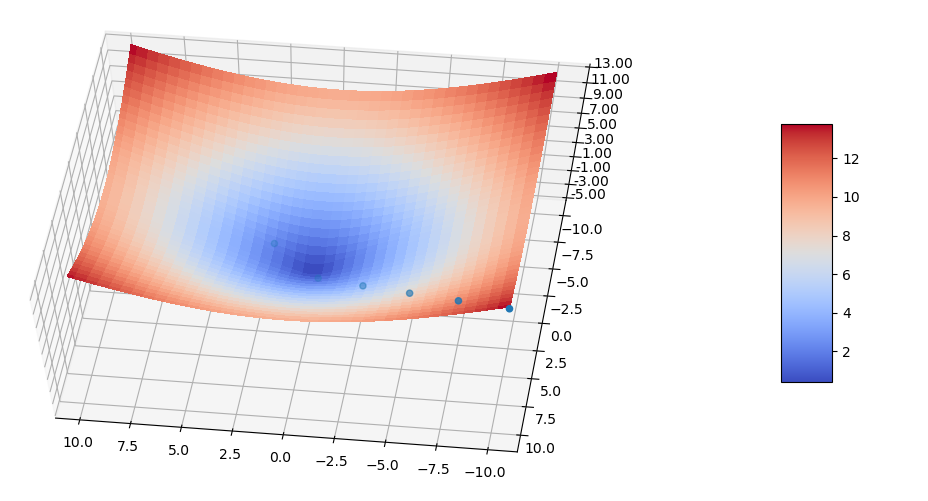
\includegraphics[scale=0.4]{images/3dgradient_descent.png}}
  	\caption{The loss function graph of multiple variables function and Gradient Descent process.}
  	\label{fig:3dgradient_descent}
\end{figure}
For $ \mu $ is the \emph{learning rate}, $ {\mu} {\in} {\mathbb {R}} $, $ {\mu}> 0 $. If we choose a large value of $ \mu $ we will need fewer number of steps to get closer to the desired minimum position but in many cases the deviation between the position of the last calculated point and the position of the the minimum point will be relatively high. Conversely, if we choose a small value of $ \mu $, we will need more steps but the offset of the distance between the position of the last calculated point and the position of the minimum point can be.

The Gradient Descent method commonly used to update weights for multivariate loss function is \emph{Mini-batch Gradient Descent}. A mini-batch will have $ n $ points with $ 1 <n {\leq} N $, $ N $ is the total number of points of the input data set. Dividing the original set of points into batches will be done randomly. Every time the algorithm finishes processing a batch will be an iteration and after all the batches are processed, it will be an epoch. So $ no\_batch = \frac {N} {n} $.

\subsubsection{Stop condition of the algorithm}
We already know the Gradient Descent algorithm will need to do a lot of computational loops to be able to converge. However it is difficult to tell when the algorithm can be stopped. In fact there are different ways used to select the calculation step number:
\begin{itemize}
	\item Selects a certain number of iteration based on the criteria such as the amount of input data. This has a drawback that it is possible for the final model to be the sub optimal and the optimal point of the model occurs in the earlier or later period of the training.
	\item Examines the change of the loss function between two consecutive updates, if the deviation reaches below a certain threshold, the algorithm is discontinued. However if on the graph of the loss function there is a flat area but the area is no where near the minimum point, the algorithm will stop in this region without achieving the minimum.
	\item Examines the shift of gradient between two consecutive updates, if the deviation falls below a threshold that is small enough, the algorithm is discontinued. The downside to this method is that the calculation of the gradient of complex function is difficult to implement.
	\item Examines the result of the algorithm to stop the iteration. This requires the person who performs the model training to regularly check the algorithm's performance parameters on a \emph{validation set} to see at which point the model produces the best performance.
\end{itemize}
The last method will be used during the training of the artificial neural network model in this paper.

With a multi-layer neural network, the loss function $J \left({\boldsymbol{W}}, {\boldsymbol{b}}, {\boldsymbol{X}}, {\boldsymbol{Y}}\right) $ will depend on the set of $ \boldsymbol{W} $ weight matrices and the bias vectors of each layer $ \boldsymbol{b} $. The calculation of the gradient of loss depends on the calculation of individual derivative $ {\frac{{\partial}J}{{{\partial}\boldsymbol{W}} ^ {(k)}}} $; $ {\frac{{\partial}J}{{\partial}\boldsymbol{b} ^ {(k)}}} $, $ {\forall}k = 1.2,.., N $. For $N $ is the number of the inputs. Notices that the individual derivative of $J $ for $ {\boldsymbol{W}} $ and $ {\boldsymbol{b}} $ is very difficult to calculate because the equation of $J $ is not directly dependent on $ {\boldsymbol{W}} $ and $ {\boldsymbol{b}} $. To be able to implement the Gradient Descent algorithm, the method commonly used is \emph{backpropagation}.
\subsubsection{Using backpropagation to implement Gradient Descent algorithm in artificial neural network}
Instead of updating all weights at the same time, Backpropagation\cite[p.220-226]{tiep:2017} will update the weights and biases from the last layer to the first layer. First the algorithm will calculate the derivative of the loss function according to the weight matrix of the last layer.
\begin{align*}
	\frac
		{ {\partial} J }
		{ {\partial} {w_{ij}^{(k)}} }
	&=
	\frac
		{ {\partial} J }
		{ {\partial} {z_{j}^{(k)}} }
	{\cdot}
	\frac
		{ {\partial} {z_{j}^{(k)}} }
		{ {\partial} {w_{ij}^{(k)}} } \\
	&=
	{e_{j}^{(k)}}
	\frac
		{ {\partial} \left(
						{w_{ij}^{(k)T}}
						a^{(k-1)}
						+
						{b_{j}^{(k)}}
					 \right)
		}
		{ {\partial} {w_{ij}^{(N)}} } \\
	&={e_{j}^{(k)}}{a_{i}^{(k-1)}} \\ \\
	\frac
		{ {\partial} J }
		{ {\partial} {b_{j}^{(k)}} }
	&=
	\frac
		{ {\partial} J }
		{ {\partial} {z_{j}^{(k)}} }
	{\cdot}
	\frac
		{ {\partial} {z_{j}^{(k)}} }
		{ {\partial} {b_{j}^{(k)}} } \\
	&={e_{j}^{(k)}}
\end{align*}
$e_{j} ^ {(k)} $ can be calculated as following:
\begin{align*}
	{e_{j}^{(k)}}
	&=
	{\frac
		{ {\partial} J }
		{ {\partial} {z_{j}^{(k)}} }
	}
	=
	{\frac
		{ {\partial} J }
		{ {\partial} {a_{j}^{(k)}} }
	}
	{\cdot}
	{\frac
		{ {\partial} {a_{j}^{(k)}} }
		{ {\partial} {z_{j}^{(k)}} }
	} \\
	&=\left( 
			 {\sum_{l=1}^{d^{(k+1)}}} 
			 {\frac
			 	{ {\partial} J }
			 	{ {\partial} {z_{l}^{k+1}} } 
			 }
			 {\cdot}
			 {\frac
			 	{ {\partial} {z_{l}^{(k+1)}} }
			 	{ {\partial} {a_{j}^{(k)}} } 
			 }
		\right) 
		{
			{f^{(k)'}} \left( 
					{z_{j}^{(k)}} 
				 \right)
		} \\
	&=\left( 
			 {\sum_{l=1}^{d^{(k+1)}}} 
			 e_{l}^{(k+1)}
			 {\cdot}
			 w_{jl}^{(k+1)}
		\right) 
		{
			{f^{(k)'}} \left( 
					{z_{j}^{(k)}} 
				 \right)
		}
\end{align*}
$f: {\mathbb{R}}{\rightarrow} [0.1] $ is the activation function, $a_{j}^{k}=f\left(z_{j}^{k}\right)$, because the partial derivative of  $a_{j}^{k}$ in accordance with $z_{j}^{k}$ is the derivative of $f$. In addition, because  $a_{j}^{k}$ is directly involved in calculating $z_{l}^{k+1},l=1,2,..,d^{(k+1)}$ so ${\frac{{\partial}J}{{\partial}{a_{j}^{k}}}}$ can be separated into the sum of partial derivative functions such as the second line. Likewise, we can calculate $
	\frac
		{ {\partial} J }
		{ {\partial} {b_{j}^{(k)}} }
	= {e_{j}^{(k)}}
$
The calculation of ${e_{j}^{k}}$ will depend on the result of ${e_{j}^{k+1}}$ so this method is called backpropagation.
The steps for implementing the backpropagation algorithm for an artificial neural network include:
\begin{enumerate}
	\item Feedforward: For each input value of x, calculate the output value of neural networks, at the same time save the results $ {\boldsymbol{a}} ^ {(k)} $ at each layer.
	\item For every $j$\emph{th} node in the output layer:
\begin{equation}
	{e_{j}^{(N)}}
	=
	\frac
		{ {\partial} J }
		{ {\partial} {z_{j}^{(N)}} }
\end{equation}
	\item Then:
\begin{align*}
	\frac
		{ {\partial} J }
		{ {\partial} {w_{ij}^{(N)}} }
	&=
	{a_{i}^{(N-1)}}
	{e_{j}^{(N)}} \\
	\frac
		{ {\partial} J }
		{ {\partial} {b_{j}^{(N)}} }
	&=
	{ e_{j}^{(N)} }
\end{align*}
	\item For $k=N-1,N-2,...,1$ calculate $e_{j}^{(k)}$
\begin{equation}
	e_{j}^{(k)}
	=
	\left( 
		{\sum_{l=1}^{d^{(k+1)}}}
		e_{l}^{(k+1)}
		{\cdot}
		w_{jl}^{(k+1)}
	\right) 
	{
		{f^{(k)'}} 
		\left( 
			{z_{j}^{(k)}} 
	 	\right)
	}
\end{equation}
	\item Update the derivative for each weight and bias:
\begin{align*}
	\frac
		{ {\partial} J }
		{ {\partial} {w_{ij}^{(k)}} }
	&=
	{a_{i}^{(k-1)}}
	{e_{j}^{(k)}} \\
	\frac
	{ {\partial} J }
		{ {\partial} {b_{j}^{(k)}} }
	&=
	{ e_{j}^{(k)} }
\end{align*}
\end{enumerate}

\subsection{Convolutional neural network}
The convolutional neural network \cite{CNN:2020:Standford} is a type of neural network used exclusively for visual problems. The convolutional neural network still has the neurons with the weights and biases that can be updated to learn the features of the image. The classes of the convolutional neural networks are arranged in three dimensions: width, height, depth. The depth here is the depth of the domain of the activation neurons rather than the depth of the whole neuron network. The neurons in the posterior layer will only be connected to a fraction of the neuron in the previous layer rather than fully connected layer in conventional neuron networks. For example CIFAR-10 Network in figure \ref{fig:CNN}, the domain of the neuron enabled in this neural network is the dimension of $32 {\times}32{\times}3 $ (\emph{width} $ {\times} $ \emph{height} $ {\times} $ \emph{depth}). The last layer of the CIFAR-10 will be the dimension of $1{\times}10{\times}10 $ corresponds to the class scores.
\begin{figure}[ht]
	\centerline{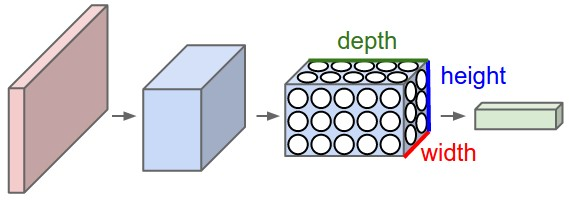
\includegraphics[scale=0.3]{images/cnn.jpeg}}
  	\caption{A simple convolutional neural network model. The image recognition layer (in red) is a three-dimensional layer with width and height that is the width and height of the input image, the value of depth is three corresponding to three color channels of red, green and blue. The layer of the convolutional neural network will transform a group of matrices into a group of other matrices. The outermost layer is the classification layer, which corresponds to a class scores vector.}
  	\label{fig:cnn}
\end{figure}
A convolutional neural network is composed of three types of layer \cite[p.113:123]{tuan:2019}: convolutional layer, pooling layer, and fully-connected layer.
\subsubsection{Convolutional layer}
In these layers, the first layer would be an input of color image with three color channels: red, green, blue like in figure \ref{fig:image_convol_0}). The output of the previous layer becomes the input of the following layer. The input and output of each convolutional layer are called tensors.
\begin{figure}[ht!]
	\centerline{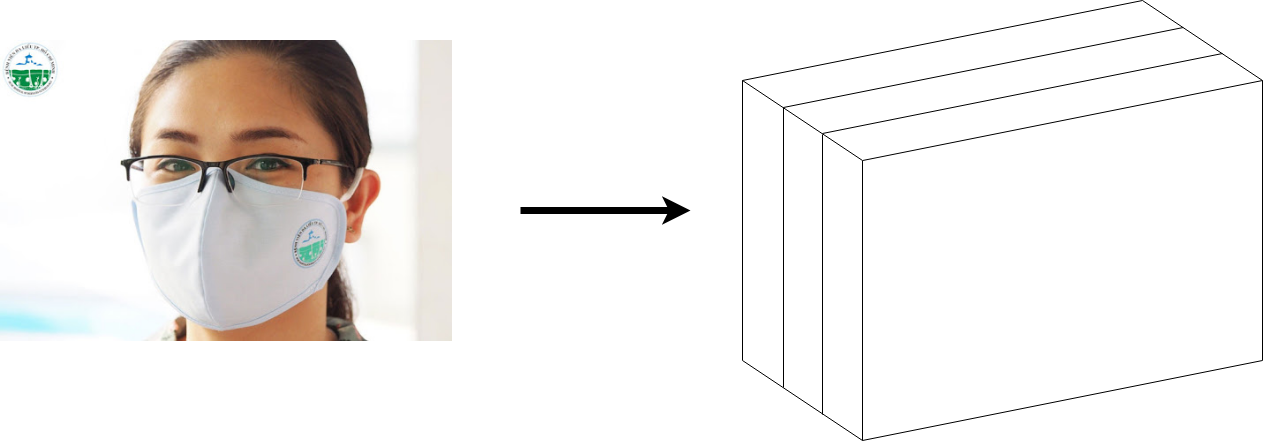
\includegraphics[scale=0.2]{images/image_convol_0.png}}
  	\caption{The input image consists of three colors channels that is modeled as a tensor with the height and the width is the height and the width of the image, depth is three.}
  	\label{fig:image_convol_0}
\end{figure}
Then a kernel of size $ m \times n \times 3 $ will slide over the tensor of the input image. In each color channel, the corresponding layer of the kernel will act as a sliding window (English: sliding window).
\begin{figure}[ht!]
	\centerline{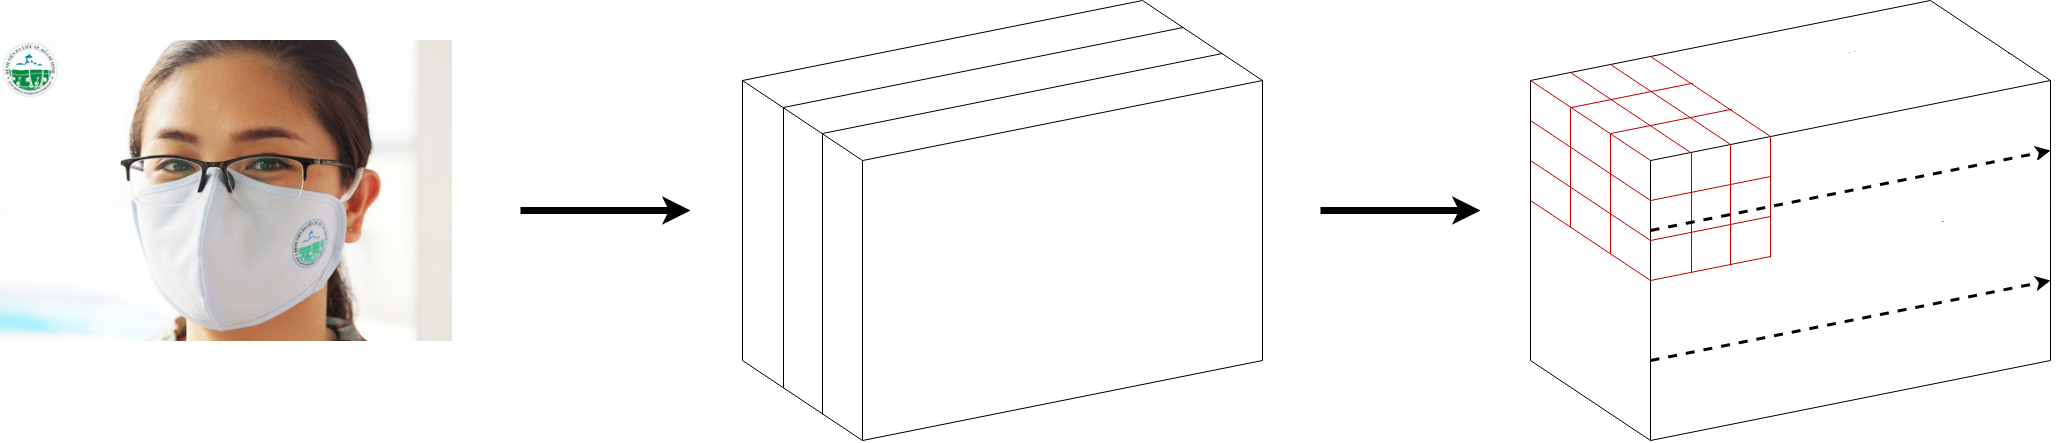
\includegraphics[scale=0.15]{images/image_convol_1.png}}
  	\caption{Image after being passed through the input and converted into three-dimensional data will be included in the first convolution layer. A kernel of size $ 3 \times 3 \times 3 $ (top left corner) is sliding over the input image.}
  	\label{fig:image_convol_1}
\end{figure}
Suppose we have a kernel of size $ 3 \times 3 \times 3 $ as shown in the figure \ref{fig:kernel}.
\begin{figure}[ht!]
	\centerline{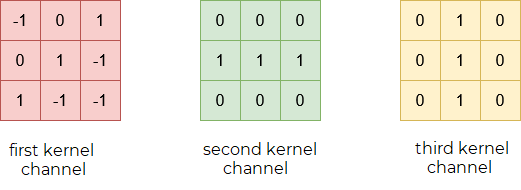
\includegraphics[scale=0.4]{images/kernel.png}}
  	\caption{A kernel of size $3 \times 3 \times 3$.}
  	\label{fig:kernel}
\end{figure}
An input image consists of three color channels, when going through the first convolution layer will be calculated as shown in figure \ref{fig:kernel_calculation}
\begin{figure}[ht!]
	\centerline{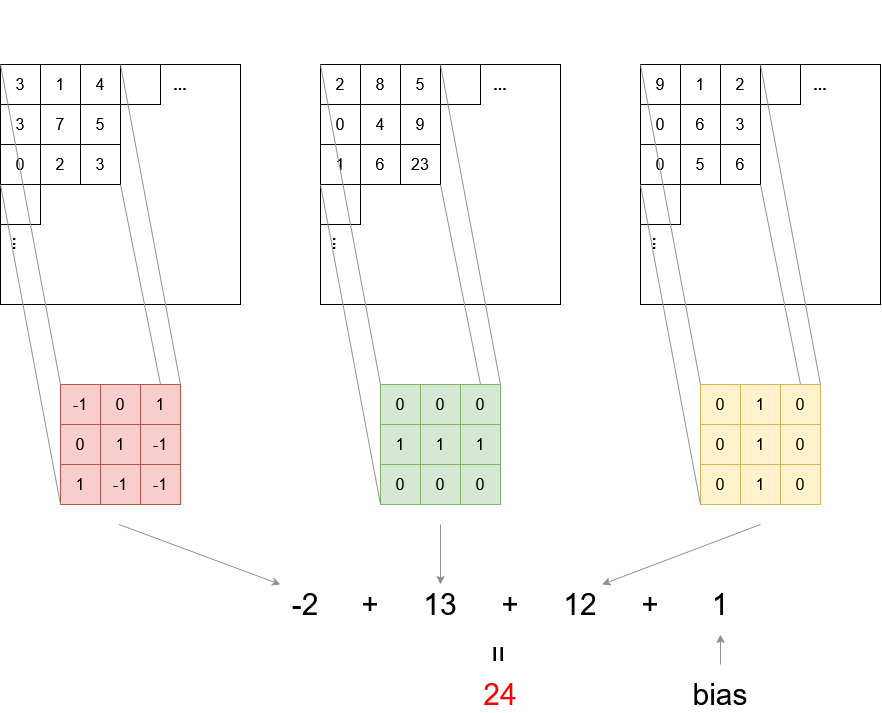
\includegraphics[scale=0.3]{images/kernel_calculation.png}}
  	\caption{Example of a kernel operation on a location of an image in a convolutional layer.}
  	\label{fig:kernel_calculation}
\end{figure}
After the kernel has scanned the desired pixels, the result will be a matrix. Each different kernel will extract a different feature of the image. So a convolutional layer will have many kernels to get different features. At this point the output will be a tensor of many matrices. If there is $ k $ kernel used at a convolution layer, the output will be as deep as $ k $, the width and height will be equal to the width and height of the input image. The output of the previous convolutional layer will be the input of the later convolutional layer.
\begin{figure}[ht]
	\centerline{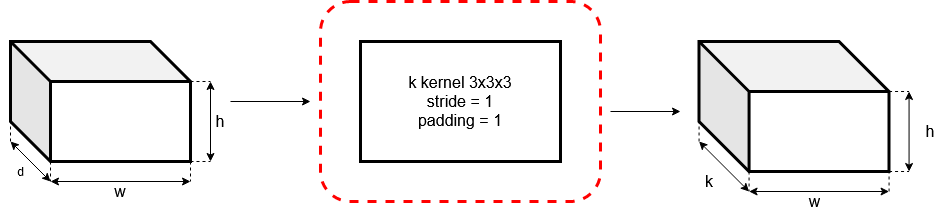
\includegraphics[scale=0.22]{images/convol_layer_in_out.png}}
  	\caption{A convolutional layer has $ k $ kernel with size $ 3 \times 3 \times 3 $, $ stride = 1 $, $ padding = 1 $. The input is a tensor of size $ h \times w \times d $, the output of the convolutional layer has the above parameters with the input provided is a tensor of size $ h \times w \times k $}
  	\label{fig:convol_layer_in_out}
\end{figure}
In general, for a convolutional layer with $ K $ kernel of size $ N \times N \times D $ (where D is the depth of input and is an odd number), $ stride = S $, $ padding = P $. If input is a tensor of size $ H \times W \times D $, then the size of output tensor will be
$\left( 
	\frac
		{{H-F+2P}}
		{S}
	+1
\right)
\times
\left( 
	\frac
		{{W-F+2P}}
		{S}
	+1
\right)
\times
K$

The output of the convolution layer will go through the activation function before being feed to the next convolution layer. Each kernel with size $ N \times N \times D $ will have a bias coefficient. The total number of parameters of a kernel is $ N \times N \times D + 1 $, with $ K $ kernels then the total number of parameters is $ K \times (N \times N \times D + 1) $.
\subsubsection{Pooling layer}
Computing with a large-resolution image as input data on a convolutional neural network is usually not computationally efficient because there are many pixels depicting the same characteristic. So pooling is used in between convolution layers to reduce the size of tensors and maintain the characteristics of the data.

For a pooling class with a sliding window size of $ N \times N $, the input is a tensor of size $ H \times W \times D $. We divide this tensor into $ D $ matrices of size $ H \times W $. For each matrix, a sliding window is applied on each pixel. In the area of the sliding window we will find the maximum or average of the values to include in the new matrix.
\begin{figure}[ht]
	\centerline{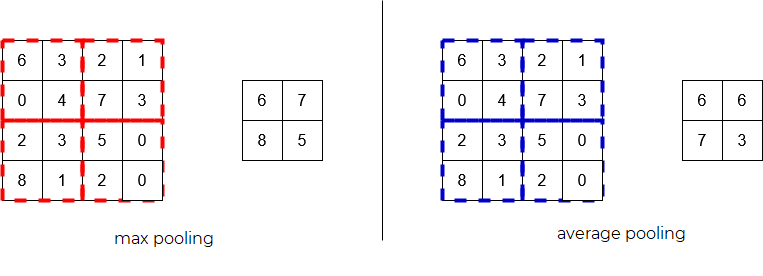
\includegraphics[scale=0.3]{images/pooling.png}}
  	\caption{On the left, the pooling layer with sliding window that returns the maximum of the values within the window region of size $ 2 \times 2, stride = 1, padding = 0 $. On the right, the pooling layer with sliding window that returns the average of the values within the window region of size $ 2 \times 2, stride = 2, padding = 0 $.}
  	\label{fig:pooling}
\end{figure}
Some convolutional neural network models will use $ stride> 1 $ in the convolution layer to reduce data size instead of pooling layer. Also, in practice pooling is often used for sliding window sizes of $ 2 \ times 2, stride = 2, padding = 0 $. The height and width of the output tensor will be reduced by half while the depth remains the same.
\subsubsection{Fully connected layer}
The image after going through convolutional layer and pooling layer produces a tensor containing the features that the model extracted. The tensor of size $ H \times W \times D $ at the last convolution layer will be converted to a vector of length $ H \times W \times D $. This vector will then be put into fully connected layers to give predictions for the image.

We can finally connect the aforementioned layers into a simple convolutional neural network as shown in figure \ref{fig:cnn_simplified}.
Input image $ \rightarrow $ [Concise layer $ \rightarrow $ Pooling class] $ \times n \rightarrow $ [Fully associative layer] $ \times m \rightarrow $ Output, with $ m, n \in { \mathbb {N}} ^ * $.
\begin{figure}[ht]
	\centerline{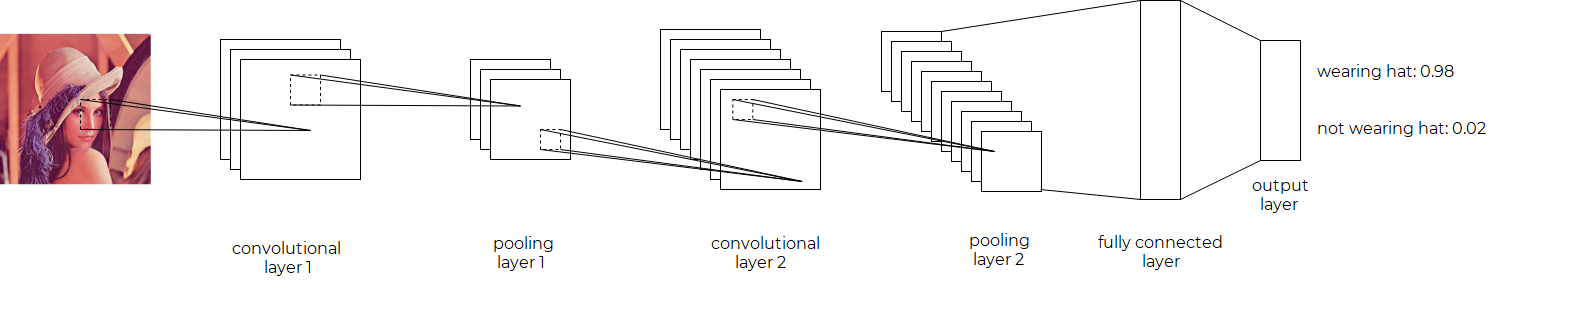
\includegraphics[scale=0.18]{images/cnn_simplified.png}}
  	\caption{The convolutional neural network consists of two convolutional layer, two pooling layers and a fully connected layer.}
  	\label{fig:cnn_simplified}
\end{figure}
\subsection{Mô hình YOLOv3}
YOLO - You Only Look Once \cite{redmod:2016:yolo} is one of the state of the art real-time detection models and is being used for many different detection problems. Unlike previous CNN or R-CNN models, instead of using the region proposal method and sliding window to detect objects in each small region in the frame and proceed to classify that object. YOLO uses all the frame to identify objects. The features of the background that is also used during training. YOLO can identify objects quickly in a frame with a high degree of accuracy with just one treatment, which is why this model is called You Only Look Once.
\subsubsection{Unified Detection}
The input image is divided into a grid cell of size $ S \times S $ like in figure \ref{fig:grid_cell}. If the center of an object is at the center of a cell, that cell is responsible for identifying the object.
\begin{figure}[ht]
	\centerline{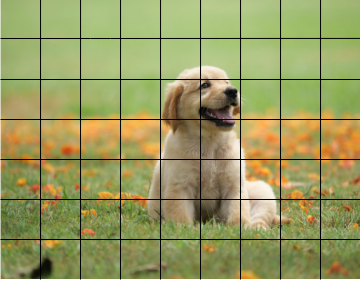
\includegraphics[scale=0.6]{images/grid_cell.png}}
  	\caption{Image is divided into grid cell of size $ S \times S $.}
  	\label{fig:grid_cell}
\end{figure}
Each box will predict the $ B $ bounding box and the confidence score of each bounding box. Let $ Pr(Object) $ be the probability of an object in a cell with $ Pr(Object) \in \mathbb {R}, 0 \leq Pr(Object) \leq 1 $. $ IOU $ - intersection over union is the ratio between the area of the intersection and the area of the union between the predicted bounding box and the ground truth bounding box figure \ref{fig:iou}, $ IOU \in \mathbb {R}, 0 \leq IOU \leq 1 $.
\begin{figure}[ht]
	\centerline{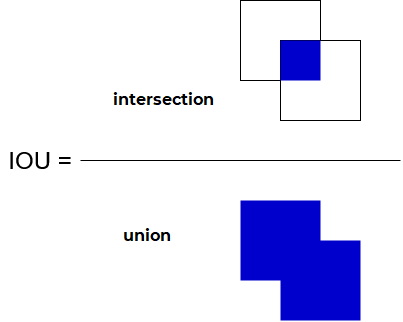
\includegraphics[scale=0.5]{images/iou.png}}
  	\caption{The IOU calculation.}
  	\label{fig:iou}
\end{figure}
The confidence is defined by $ Pr(Object) \times IOU $, if a cell does not contain an object then $ Pr(Object) = 0 $ implies that confidence will be zero, otherwise if a cell contains the object, $ Pr (Object) = 1 $, then the confidence is $ IOU $.

Each bounding box will have five parameters to predict: $ t_x, t_y, t_w, t_h $ and confidence score. $ (t_x, t_y) $ is the relative coordinates of the center bounding box to a cell, if the offset of a cell in the image is $ (c_x, c_y) $ then the coordinates of a bounding box compared to the image are $ ( \sigma \left (t_x \right) + c_x, \sigma \left( t_y \right) + c_y) $. If the length and width of the given bounding box are $ \ left (p_w, p_h \ right) $ then the length and width of the bounding box are predicted to be $ \left( p_w \times e ^ {t_w}, p_h \times e ^ {t_h} \right) $.
\begin{align*}
	b_x &= \sigma \left( t_x \right)+c_x\\
	b_y &= \sigma \left( t_y \right)+c_y\\
	b_w &= p_w \times e^{t_w}\\
	b_h &= p_h \times e^{t_h}
\end{align*}
\begin{figure}[ht]
	\centerline{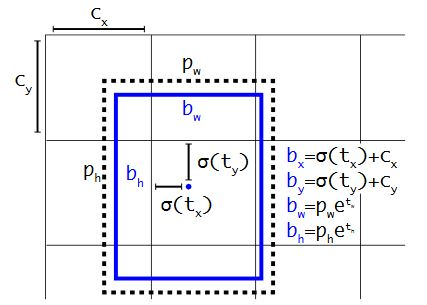
\includegraphics[scale=0.5]{images/bounding_box_prediction.jpg}}
  	\caption{YOLO's bounding box prediction model.}
  	\label{fig:bounding_box_prediction}
\end{figure}
During training, the function of the loss of the sum of squared deviations is used for the coordinates of the bounding box. For a prediction $ t_* $ with a ground truth of $ {\widehat{t}}_* $, the gradient will be the difference between ground truth and the predicted result $ {\widehat{t}}_* - t_* $.

YOLOv3 \cite{redmon:2018:yolov3} uses a logistic regression function to predict whether a bounding box contains an object. If the predicted bounding box has large intersect area with the ground truth than the previous bounding box, the result is $ 1 $. If a predicted bounding box does not have the largest area of intersection with ground truth but the still has greater confidence than a definite threshold, then the prediction will be ignored. The IOU threshold used is $ 0.5 $. If a bounding box is not placed in a ground truth, there will be no predictions on coordinates and classes, but only the existence of objects.
Confidence is the $ IOU $ between the predicted bounding box and the ground truth. For cells that are predicted to have objects, the model predicts an additional $ C $ probability of the class that the object might belongs to $Pr\left(Class_i|Object\right)$ with $ Pr \left( Class_i | Object \right) \in \mathbb{R}, 0 \leq Pr \left( Class_i | Object \right) \leq 1, i = 1,..,C $. Each cell will have only a set of values $Pr \left( Class_i | Object \right) $ that are not related to the bounding box $ B $.

When making predictions, YOLO will multiply probabilities and confidence together to get the probability of a class on a bounding box.
\begin{equation}
	Pr \left( Class_i | Object \right) \times Pr(Object) \times IOU = Pr \left( Class_i \right) \times IOU
\end{equation}
The loss function used when training to predict classes is the binary cross-entropy function to help the model to predict multiple classes in the same cell.

Finally we have the total loss function of YOLOv3
\begin{figure}[ht]
	\centerline{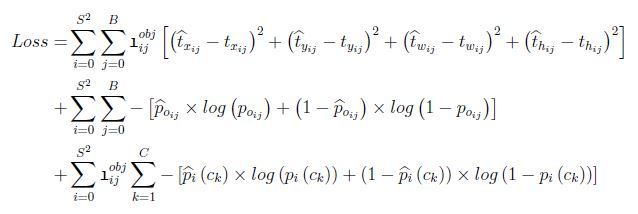
\includegraphics[scale=0.53]{images/yolov3_loss_function.jpg}}
\end{figure}
\subsubsection{YOLOv3 architecture}
Features from images are extracted in three different proportions by the same method used in pyramid networks (feature pyramid networks). The output of the extracted domain is typically a three-dimensional tensor containing the bounding box position, probability of object existence, probability of classes, tensor size is $ S \times S \times [3 \times (4 + 1 + C)] $, where $ S \times S $ is the number of cells the image is divided into, $ 4 $ is the predicted value of bounding box $ \ left (t_x, t_y, t_w, t_h \ right) $, $ 1 $ is the predicted value of the existence of the object in the cell, $C$ is the vector of predicted values of the classes.

Then the characteristic matrices from the previous two classes and up-sampled twice. In addition, specific matrices from the earlier classes are combined with the following layers. This helps the model derive a lot of meaningful information from the up-sampled featured matrices and retain smaller features from the first classes. Later several convolution layers were used to combine the characteristic matrices and produce the final tensor containing doubly sized predictions.

At the end, the model shown above is repeated many times, which allows the final bounding box to use values that have been calculated from previous layers as well as characteristics that have meaning.

Initially there will be nine bounding boxes: $ (10 \times 13), (16 \times 30), (33 \times 23), (30 \times 61), (62 \times 45), (59 \times 119) , (116 \times 90), (156 \times 198), (373 \times 326) $. These bounding boxes will be divided into three ratios using the k-means algorithm. These bounding boxes will be used to predict the corresponding proportions. The input image will be down-sample with strides equal to $ 32 $, $ 16 $ and $ 8 $ for each scale. As a result, YOLOv3 can predict small objects very well.

YOLOv3 uses a network architecture combining YOLOv2, Darknet-19 and residual networks. The convolution classes are $ 3 \times 3 $, $ 1 \times 1 $ and have extra shortcuts. The figure \ref{fig:yolov3_architechture} shows the Yolov3 architecture which has 53 convoluted layers so this architecture is called Darknet-53.
\begin{figure}[ht]
	\centerline{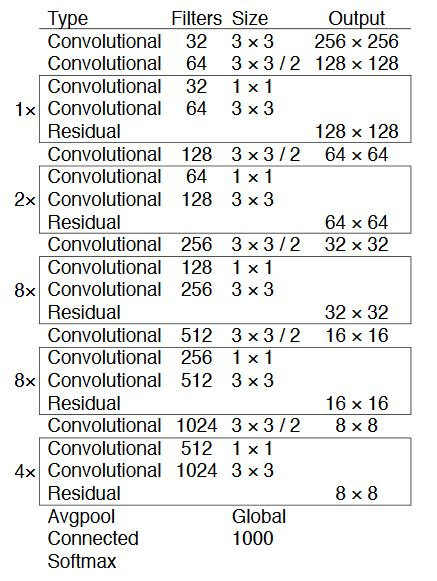
\includegraphics[scale=0.7]{images/yolov3_architecture.jpg}}
  	\caption{Darknet-53 architecture.}
  	\label{fig:yolov3_architechture}
\end{figure}
This architecture provides better detection performance than Darknet-19 and higher performance than ResNet-101 or ResNet-152 tables \ref{table:darknet-53_performance}.
\begin{center}

  \begin{tabular} {l l l l l l}
  \toprule
  \it Backbone & \it Top-1 & \it Top-5 & \it Bn Ops & \it BFLOP/s & \it FPS \\
  \midrule

  Darknet-19 & 74.1 & 91.8 & 7.29 & 1246 & \textbf{171} \\
  ResNet-101 & 77.1 & 93.7 & 19.7 & 1039 & 53 \\
  ResNet-152 & \textbf{77.6} & \textbf{93.8} & 29.4 & 1090 & 37 \\
  Darknet-53 & 77.2 & \textbf{93.8} & 18.7 & 1457 & 78 \\
          
  \bottomrule
  \end{tabular}

\captionof{table}{Compare the performance of Darknet-53 with other networks. Accuracy, Bn Ops - billions of oper-ations, BFLOP/s - billion floating point operations per second, và FPS - frames per second.
\label{table:darknet-53_performance}}
\end{center}

\section{Building data sets, training and using YOLOv3 model for the problem of identifying personal protective equipment}
\subsection{Develop a data set for the problem of detecting personal protective equipment}
The problem is to identify whether the person in the frame is wearing personal protective equipment or not. The personal protective equipment selected for identification are: hard hat, safety vest and mask.
\begin{figure}[ht]
	\centerline{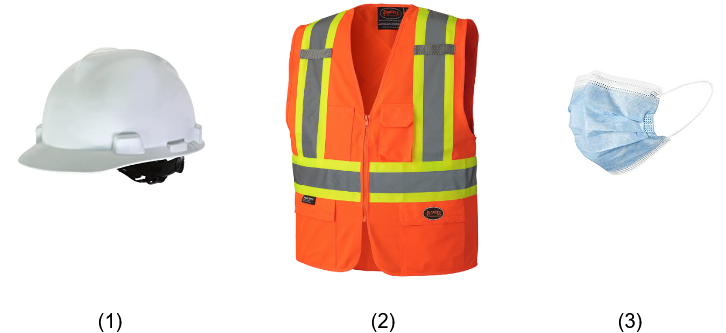
\includegraphics[scale=0.3]{images/ppe.png}}
  	\caption{(1) Hard hat, (2) Safety vest, (3) Mask}
  	\label{fig:ppe}
\end{figure}

The system's output goal is to be able to identify the position of the head and body and classify the use of personal protective equipment for detected objects. For each equipment, the object will be classified into two states, one is \emph{Wearing}, the other is \emph{Not wearing}.
\begin{itemize}
	\item Wearing a hardhat
	\item Not wearing a hardhat
	\item Wearing a safety vest
	\item Not wearing a safety vest
	\item Wearing a mask
	\item Not wearing a mask
\end{itemize}
Figure \ref{fig:expected_output} illustrates the desired output of the system.
\begin{figure}[ht!]
	\centerline{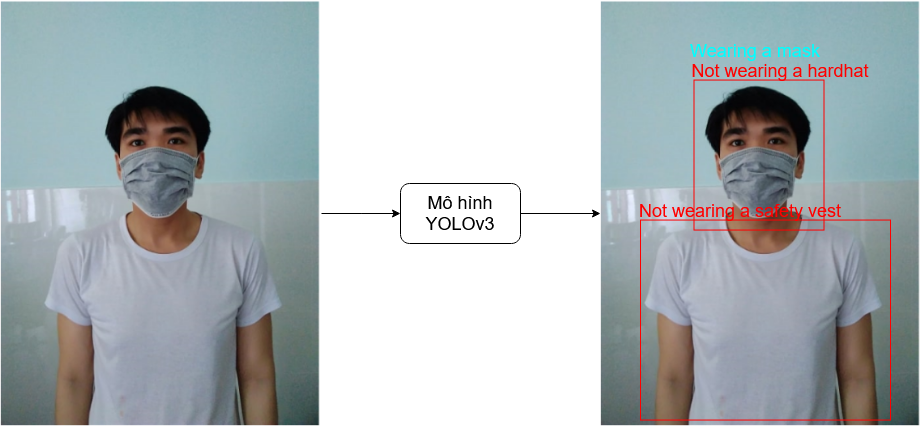
\includegraphics[scale=0.25]{images/expected_output.png}}
  	\caption{Desired output of the system.}
  	\label{fig:expected_output}
\end{figure}
The data set contains $ 11586 $ images with:
\begin{itemize}
	\item $3541$ images taken from the dataset \emph{Hardhat and Safety Vest Image for Object Detection}\cite{john:2020:hardhat}
	\item $3174$ images taken from the dataset \emph{GDUT-HWD}\cite{jixiu:2019:automatic}
	\item $4871$ images taken from image search engine \emph{Google image}
\end{itemize}

Images are labeled with the software \emph{LabelImg} \cite{tzu:2018:labelimg}. Each image will have a corresponding text file with the \emph{.txt} extension. Inside this file are labels marked with the YOLO format with information including \emph{object class id} - this is the id corresponding to the order of a label in the list of labels, \emph{x} and \emph{y} are the relative coordinates of the bounding box marked with the image, \emph{w} and \emph{h} are the relative width and height of the bounding box marked with the image, the figure \ref{fig:yolo_annotation}.
\begin{figure}[ht]
	\centerline{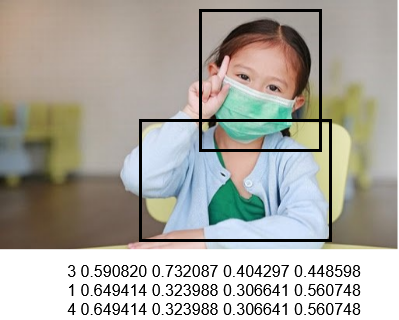
\includegraphics[scale=0.6]{images/yolo_annotation.png}}
  	\caption{YOLO annotation format.}
  	\label{fig:yolo_annotation}
\end{figure}
This data set has a total of \textbf{195771} objects labeled with the number of objects for each class shown in figure \ref{fig:object_count}.
\begin{figure}[ht]
	\centerline{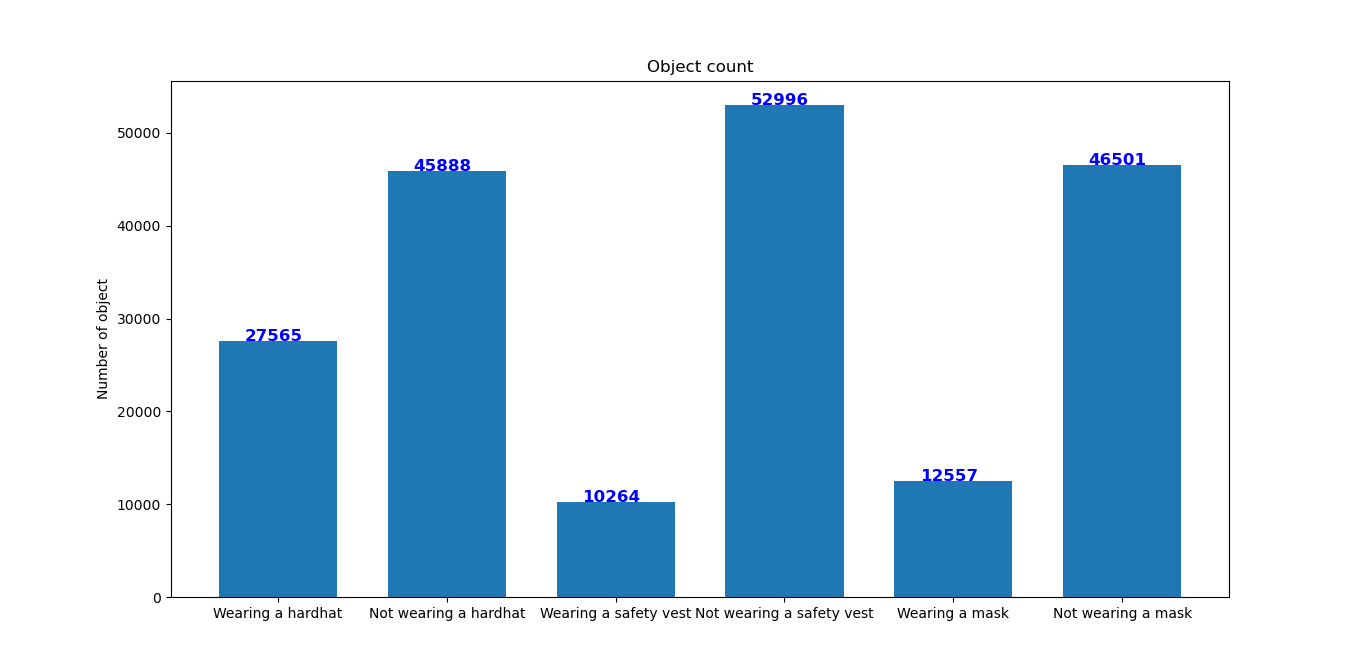
\includegraphics[scale=0.3]{images/object_count.png}}
  	\caption{Number of objects corresponding to each class. Wearing a hardhat: $27565$, Not wearing a hardhat: $45888$, Wearing a safety vest: $10264$, Not wearing a safety vest: $52996$, Wearing a mask:$12557$, Not wearing a mask: $46501$.}
  	\label{fig:object_count}
\end{figure}

The large difference in the number of bounding boxes between specific classes is that the \emph{Not wearing} classes are much larger than the corresponding \emph{Wearing} classes that will help the detector to be more sensitive to cases of violating labor protective clothing. Although there are large differences, the number of bounding boxes of each class is large enough for the model to learn the necessary characteristics to be able to correctly classify classes for a bounding box.
\subsection{Training with darknet}
Darknet \cite{alexey:2020:darknet} is a framework built by Joseph Redmon who is also the father of YOLO, this framework is written in C/C++ and is used to train the YOLOv3 model with specific data set for each problem. YOLOv3 model is trained on $ Google Colab $, which is a virtual machine environment running Linux with the configuration of
\begin{itemize}
	\item Operating System: Ubuntu 18.04.3 LTS
	\item CPU: Intel 2-core Xeon 2.2GHz
	\item RAM: 13Gb
	\item HDD: 33Gb
	\item GPU: Tesla K80 with 12GB memory
\end{itemize}

To be able to train the YOLOv3 model for custom data set, we need to perform a few configuration steps.
\begin{enumerate}
	\item We copy the file \emph{yolov3.cfg} in the \emph{cfg} directory to the \emph{darknet} working directory and edit the following. \emph{subdivision} is the parameter to split a mini-batch to ensure the model can run on different GPU resources, because the data set contains many different sized images, so in the training process, if \emph{subdivision} is small, it is easy to get the error \emph{out of memory} so after trying many different values such as $ 16, 32, 64 $ then $ 64 $ allows the training to take place without any problem. In return, the training time will be longer because it is not possible to put multiple images at the same time for training. \emph{width} and \emph{height} are the width and height of the input image, the images of different sizes will be resized before being used for training. To ensure the image after resizing does not loose too much information, and make sure the training is possible on the GPU resources provided so \emph{width} and \emph{height} are selected as $ 608 $. The choice of \emph{max{\_}batches} is the total number of batches the model will run, this is also known as the number of \emph{iteration}, we can choose \emph{max{\_}batches} are very large and rely on \emph{mAP} or \emph{average loss} to stop the algorithm, but after training the model a few times it shows that \emph{max{\_}batches} should be roughly larger than the number of classes multiplied by $ 2000 $ but not less than the number of images in the training data set. \emph{steps} will have values of $ 80 \% $ and $ 90 \% $ respectively of \emph{max{\_}batches}.
	
\noindent\fbox{
    \parbox{210pt}{
        \texttt{\#} [net]\\
		\texttt{\#} Testing\\
		\texttt{\#} batch=1\\
		\texttt{\#} subdivisions=1\\
		\texttt{\#} Training\\
		batch=64\\
		subdivisions=64\\
		width=608\\
		height=608\\
		channels=3\\
		momentum=0.9\\
		decay=0.0005\\
		angle=0\\
		saturation = 1.5\\
		exposure = 1.5\\
		hue=.1\\
\\
		learning{\_}rate=0.001\\
		burn{\_}in=1000\\
		max{\_}batches = 22000\\
		policy=steps\\
		steps=17600,19800\\
		scales=.1,.1\\
    }
}
\\
Then at lines $ 610, 696 $ and $ 783 $ we will replace the number of $ classes $ with six, which is the class number of the problem. At the same time, we will fix the $ filters $ number of the convolution layer right above by the formula $ 3 \times (5 + C) $ where $ C $ is the class number, $ 3 $ is the number of scales the model will predict, $ 5 $ includes $ 4 $ parameter coordinates of the bounding box and $ 1 $ parameters predict the existence of the object in that bounding box, when $ C = 6 $ we have $ filters = 33 $.

\noindent\fbox{
    \parbox{210pt}{
		[convolutional]\\
		size=1\\
		stride=1\\
		pad=1\\
		filters=33\\
		activation=linear\\
\\
		\text{[yolo]}\\
		mask = $0,1,2$\\
		anchors = $10,13,16,30,33,23,30,61,62,45,59,119,$ \\ 
		$116,90,156,198,373,326$\\
		classes=6\\
		num=9\\
		jitter=.3\\
		ignore{\_}thresh = .7\\
		truth{\_}thresh = $1$\\
		random=$1$\\
	}
}

	\item Edit the parameters at the top of the file \emph{Makefile} as follows. OpenCV and GPU will be used during training and prediction so these two values are set as $ 1 $.

\noindent\fbox{
    \parbox{210pt}{
		GPU=1\\
		CUDNN=0\\
		CUDNN{\_}HALF=0\\
		OPENCV=1\\
		AVX=0\\
		OPENMP=0\\
		LIBSO=0\\
		ZED{\_}CAMERA=0 \# ZED SDK 3.0 and above\\
		ZED{\_}CAMERA{\_}v2{\_}8=0 \# ZED SDK 2.X\\
	}
}

	\item Create a file named $ obj.names $ containing the class names.

\noindent\fbox{
    \parbox{210pt}{
		Wearing a hardhat\\
		Not wearing a hardhat\\
		Wearing a safety vest\\
		Not wearing a safety vest\\
		Wearing a mask\\
		Not wearing a mask\
	}
}

	\item Copy the data set containing images and the file labeled into the path \emph{./data/objects}

	\item Create two text files, \emph{train.txt} and \emph{val.txt} that contain links to images. \emph{train.txt} is used to train and \emph{val.txt} will be used to validate the model during training. The data set is randomized. There are \textbf{900} images used for validation and \textbf{10686} images used for training. This division is done by a Python program.

	\item The weight file from the Imagenet network - \emph{darknet53.conv.74} has been trained through millions of images so the weights of the convolution layers have been optimized to extract the feature from the image. Therefore, we will reuse the weights in the cumulative classes of this weight file and only train the weights of the fully connected class for the thesis problem. This is a very common practice because it allows inheriting the very good identification performance of YOLO into many different identification problems.
	
	\item Compress the working directory into a \emph{zip} file, create a directory named \emph{Darknet} on \emph{Google Drive} and upload the compressed file into this directory. Also create a subdirectory called \emph{backup} in \emph{Darknet}.
	
	\item In \emph{Google Colab}, select \emph{Runtime} $ \rightarrow $ \emph{Change runtime type} $ \rightarrow $ \emph{Hardware accelerator} $ \rightarrow $ \emph{GPU}, run the following code to \emph{build Darknet}.

\noindent\fbox{
    \parbox{210pt}{
	from google.colab import drive\\
	drive.mount('/content/drive')\\
	{\%}cd /content\\
	!unzip /content/drive/'My Drive' \\ \tab /Darknet/darknet.zip\\
	{\%}cd /content/darknet\\
	!sudo apt-get install dos2unix\\
	!make\\
	!chmod +x ./darknet\\
	!rm /content/darknet/backup -r\\
	!ln -s /content/drive/'My Drive' \\ \tab /Darknet/backup /content/darknet\\
	{\%}cd /content/darknet\\
	!find . -type f -name "*.txt" \\ \tab -print0 | xargs -0 dos2unix\\
	}
}

	\item For the first time we will run the following command.
	
\noindent\fbox{
    \parbox{210pt}{
	!./darknet detector train obj.data \\ \tab yolov3.cfg darknet53.conv.74
	}
}	

	For the next training we just need to use the file \emph{yolov3{\_}last.weights} to continue the training without retraining from the beginning.
	
\noindent\fbox{
    \parbox{210pt}{
	!./darknet detector train obj.data \\ \tab yolov3.cfg ./backup/yolov3{\_}last.weights
	}
}

	\item \emph{Darknet} will automatically save weight files per $ 1000 $ \emph{iteration} for example: \emph{yolov3{\_}1000.weights}, \emph{yolov3{\_}2000.weights} . We can stop the training to test the model's performance parameters like \emph{precision} and \emph{recall}. This test is performed on the validate dataset in the file \emph{val.txt}. To perform this check we will run the following command.
	
\noindent\fbox{
    \parbox{210pt}{
	!./darknet detector map obj.data \\ \tab yolov3.cfg ./backup/yolov3{\_}1000.weights
	}
}

	We can replace \emph{yolov3{\_}1000.weights} with the weight file we want to check.
\end{enumerate}
\subsection{Use Python and a trained deep learning model to detect the use of personal protective equipment on camera or video}
After the training is completed, we will use the weight file to carry out identification on video or camera. To do this, we will write a Python program with a block diagram like the figure \ref{fig:flow_chart}.
\begin{figure}[ht]
	\centerline{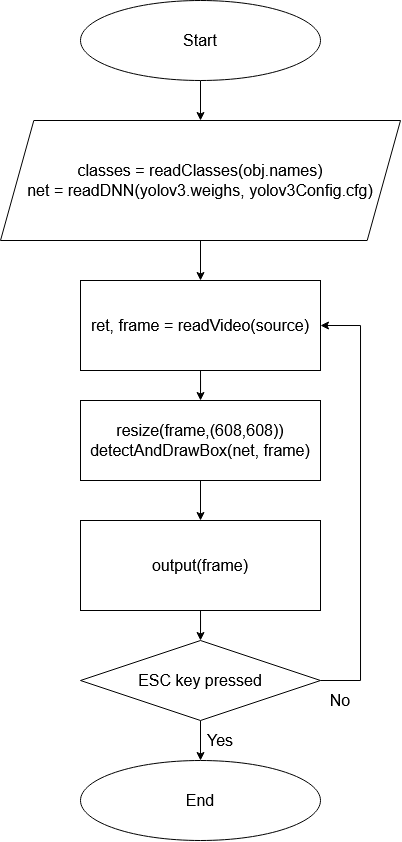
\includegraphics[scale=0.5]{images/flow_chart.png}}
  	\caption{Python flowchart diagram for detection on video or webcam.}
  	\label{fig:flow_chart}
\end{figure}
\begin{enumerate}
	\item The program will take the names of classes defined in the \emph{obj.names} file, and will also read the model's weight values in the \emph{yolov3.weights} file based on the parameters of The architecture is already installed in the file \emph{yolov3Config.cfg}. The function to read the DNN model in OpenCV is \emph{cv2.dnn.readNet(weightsFile, configFile)} with \emph{weightsFile} as the weight file and \emph{configFile} is the architecture file of the network.
	
	\item Then we will use the video reading function of OpenCV to read data from the webcam. First we will initialize an object that represents the webcam \emph{cap = VideoCapture(0)}. We will then read each frame from the newly created object \ emph{ret, image = cap.read()} where \emph{image} is a variable containing a frame, \emph{ret} will have the value \emph{True} if any frame is read from the input and \emph{False} if no frame is read from the input.
	
	\item To perform detection on the image, we will use the following command.

\noindent\fbox{
    \parbox{210pt}{
    blob = cv2.dnn.blobFromImage(image, scale, \\ \tab (604, 604), (0, 0, 0), True, crop=False)\\
	net.setInput(blob)\\
    outs = net.forward(get{\_}output{\_}layers(net))\\
	}
}

	The first command line will resize the image to size $ (604, 604) $, currently the cameras usually have 2MP resolution with a frame size of $ 1920 \times 1080 $ so resizing to $ 604 \times 604 $ will does not lose important features and allows to reduce the number of calculations so that image prediction is faster and requires less hardware resources. Each pixel in the image is then subtracted for $ (0, 0, 0) $ and divided by \emph{scale}. \emph{swapRB = True} will swap the positions of the two red and blue channels in the tensor of the figure. \emph{crop = False} will not crop the image after resizing. Assuming the red channel of the image after resizing is $ R $, \emph{scale} $ = \sigma $, the subtracted value is $ {\mu}_{red} $, the channel value The red color after passing through the \emph{blob} function will be
\begin{equation}
	\frac{R-{\mu}_{red}}{\sigma}
\end{equation} 
	The result of the function \emph{blob} will be put into the object \emph{net} and the output will be the result of the feed forward process.
	
	\item However, at \emph{outs} there will be a lot of duplicate bounding boxes due to the same object and class. Therefore the output needs to go through the non-maximum suppression algorithm in order to obtain a separate and unique bounding box for an object.
	
	Basically the non-maximum suppression algorithm works as follows.
	\begin{enumerate}
		\item Beginning the algorithm there will be two one-dimensional arrays A and B with array A containing the bounding boxes to handle, array B empty.
		\item Take the bounding box with the largest \emph{confidence} value in A and put it in B and remove the bounding box from A.
		\item For every remaining bounding box in A, find the IOU with the bounding box just inserted in B. If the IOU is greater than the threshold \emph{nmsThreshold}, then the bounding type is being removed out of A.
		\item Repeat steps (b) and (c) until there are no bounding boxes in A.
	\end{enumerate}

\noindent\fbox{
    \parbox{210pt}{
	indices = cv2.dnn.NMSBoxes(boxes, \\ \tab confidences, confThreshold, nmsThreshold)
	}
}

	\item Finally, we'll draw bounding boxes into the frame and output to the screen.
\end{enumerate}
\section{evaluation}
The model trained for three days for $ 12000 $ iteration. During training, the calculation of the model's performance parameters is performed for every $ 1000 $ iteration on the validation data set.
Recalling how to calculate performance parameters:
\begin{itemize}
	\item Precision is a parameter representing the precision of the predictions. $ True Positive $ (abbreviated: TP) are bounding boxes that are properly and truly predicted. $ False Positive $ (abbreviated: FP) are bounding boxes that are properly predicted and not really true. Precision is calculated using the following formula
	\begin{equation}
		precision = \frac{TP}{TP+FP}.
	\end{equation}
	\item Recall is a parameter that shows the model's sensitivity to objects that need to be identified. $ True Positive $ (abbreviated: TP) are bounding boxes that are properly and truly predicted. $ False Negative $ (abbreviated: FN) are bounding boxes that are predicted incorrectly or unlabeled and are actually true. Recall is calculated by the following formula
	\begin{equation}
		precision = \frac{TP}{TP+FN}.
	\end{equation}
	\item Average precision is the parameter calculated for a class. For each class, during evaluation on the validation data set, precision and recall values are saved. We will then draw a graph of precision according to recall, the average precision of a class will be the area under this graph. Call $ p (r): [0,1] \rightarrow [0,1] $ is a function that represents the relationship of precision and recall. The average precision of a class will be calculated according to the formula below
	\begin{equation}
		\text{average precision} = \int_{0}^{1} p(r) dr
	\end{equation}
	\item Mean precision precision is the average of the average precision of classes
	\begin{equation}
		\text{mean average precision} = \frac{\sum_{i=0}^{N} ap_i}{N}
	\end{equation}
	With $N \in \mathbb{N}^*$ is the class number of the model.
\end{itemize}
The validation data set consists of $ 900 $ image randomly divided from the original data set and not used for training, the number of objects in this data set is shown in Figure \ref{fig:validation_set}
\begin{figure}[ht]
	\centerline{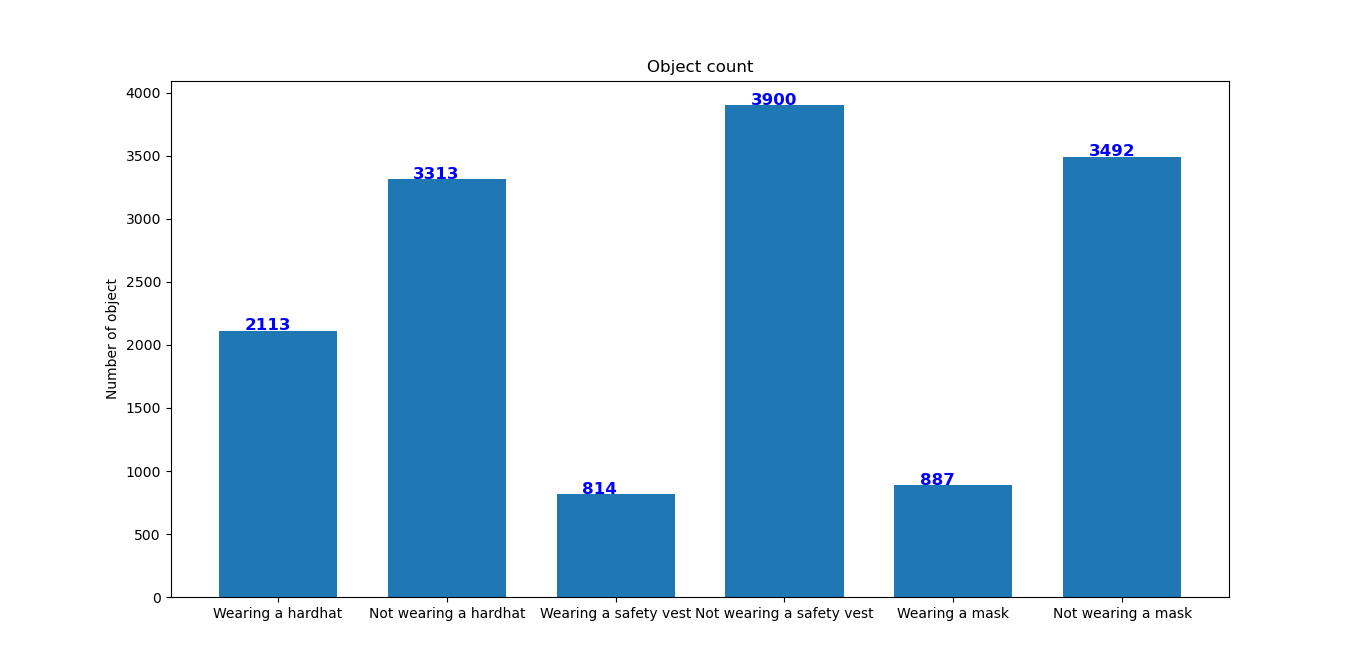
\includegraphics[scale=0.3]{images/validation_set.png}}
  	\caption{Number of objects in the validation data set. Wearing a hardhat - $2113$, Not wearing a hardhat - $3313$, Wearing a safety vest - $814$, Not wearing a safety vest - $3900$, Wearing a mask - $887$, Not wearing a mask - $3492$.}
  	\label{fig:validation_set}
\end{figure}

The calculated parameters include: precision, recall and mean average precision \ref{fig:precision_recall_map}. We find that with the amount of data from the training set, the model gives the best performance on the validation set at $ 10000 $ iteration. When looking at Internet forums as well as those who directly build the darket framework, the maximum number of iterations will usually be suggested as the number of classes $ C $ multiplied by $ 2000 $. For this model the ideal iteration number is $ 12000 $. However, based on the results on the validation set, we find that the model's performance parameters at $ 10000 $ iteration are much higher than at $ 12000 $. Therefore, in the process of training deep learning network models, the best stopping method is still to regularly check the performance of the model on a set of validation to detect optimal points.

\begin{figure}[ht!]
	\centerline{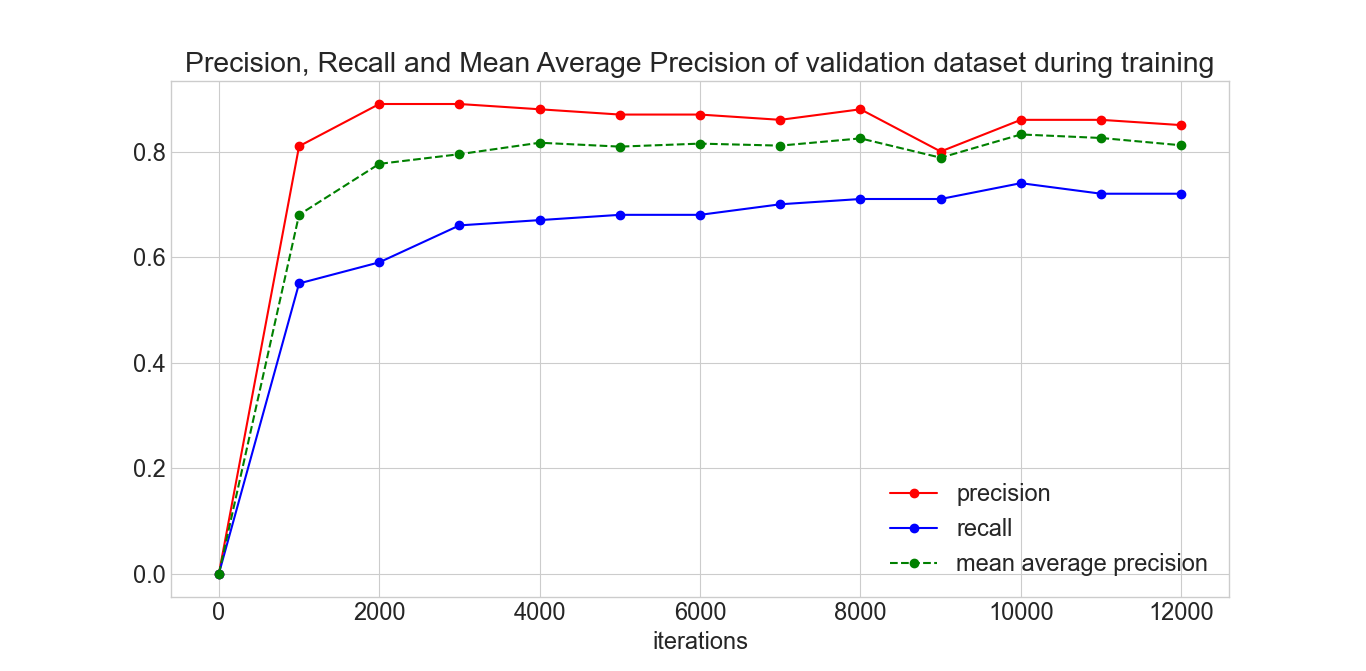
\includegraphics[scale=0.3]{images/precision_recall_map.png}}
  	\caption{Precision - red, Recall - blue, Mean Average Precision - green. The parameters are calculated every 1000 iterations on the validation data set.}
  	\label{fig:precision_recall_map}
\end{figure}

\subsubsection{Model testing in real cases}
The evaluation of the model on the validation data set also partly reflects the performance parameters of the model, but to be able to make more intuitive assessments, practical tests are needed. The following tests are carried out under different conditions and circumstances in order to investigate the model's predictive power in possible cases. Each case will be taken a number of unified images, then will use the model to make predictions on these images, then the evaluation of the model's performance parameters in the case. The images taken with the camera have an aperture of f 4.0, focal length of 14 mm.
\subsubsection{Investigate the precission and recall of the model when the distance from the camera to the subject changes}
In this experiment, the subjects will stand in turn at distances of $ 3 $ m - figure \ref{fig:3m}, $ 6 $ m - figure \ref{fig:6m} and $ 9 $ m - figure \ref{fig:9m} compared to the camera.
\begin{figure}[ht]
\centering
\begin{minipage}{0.45\textwidth}
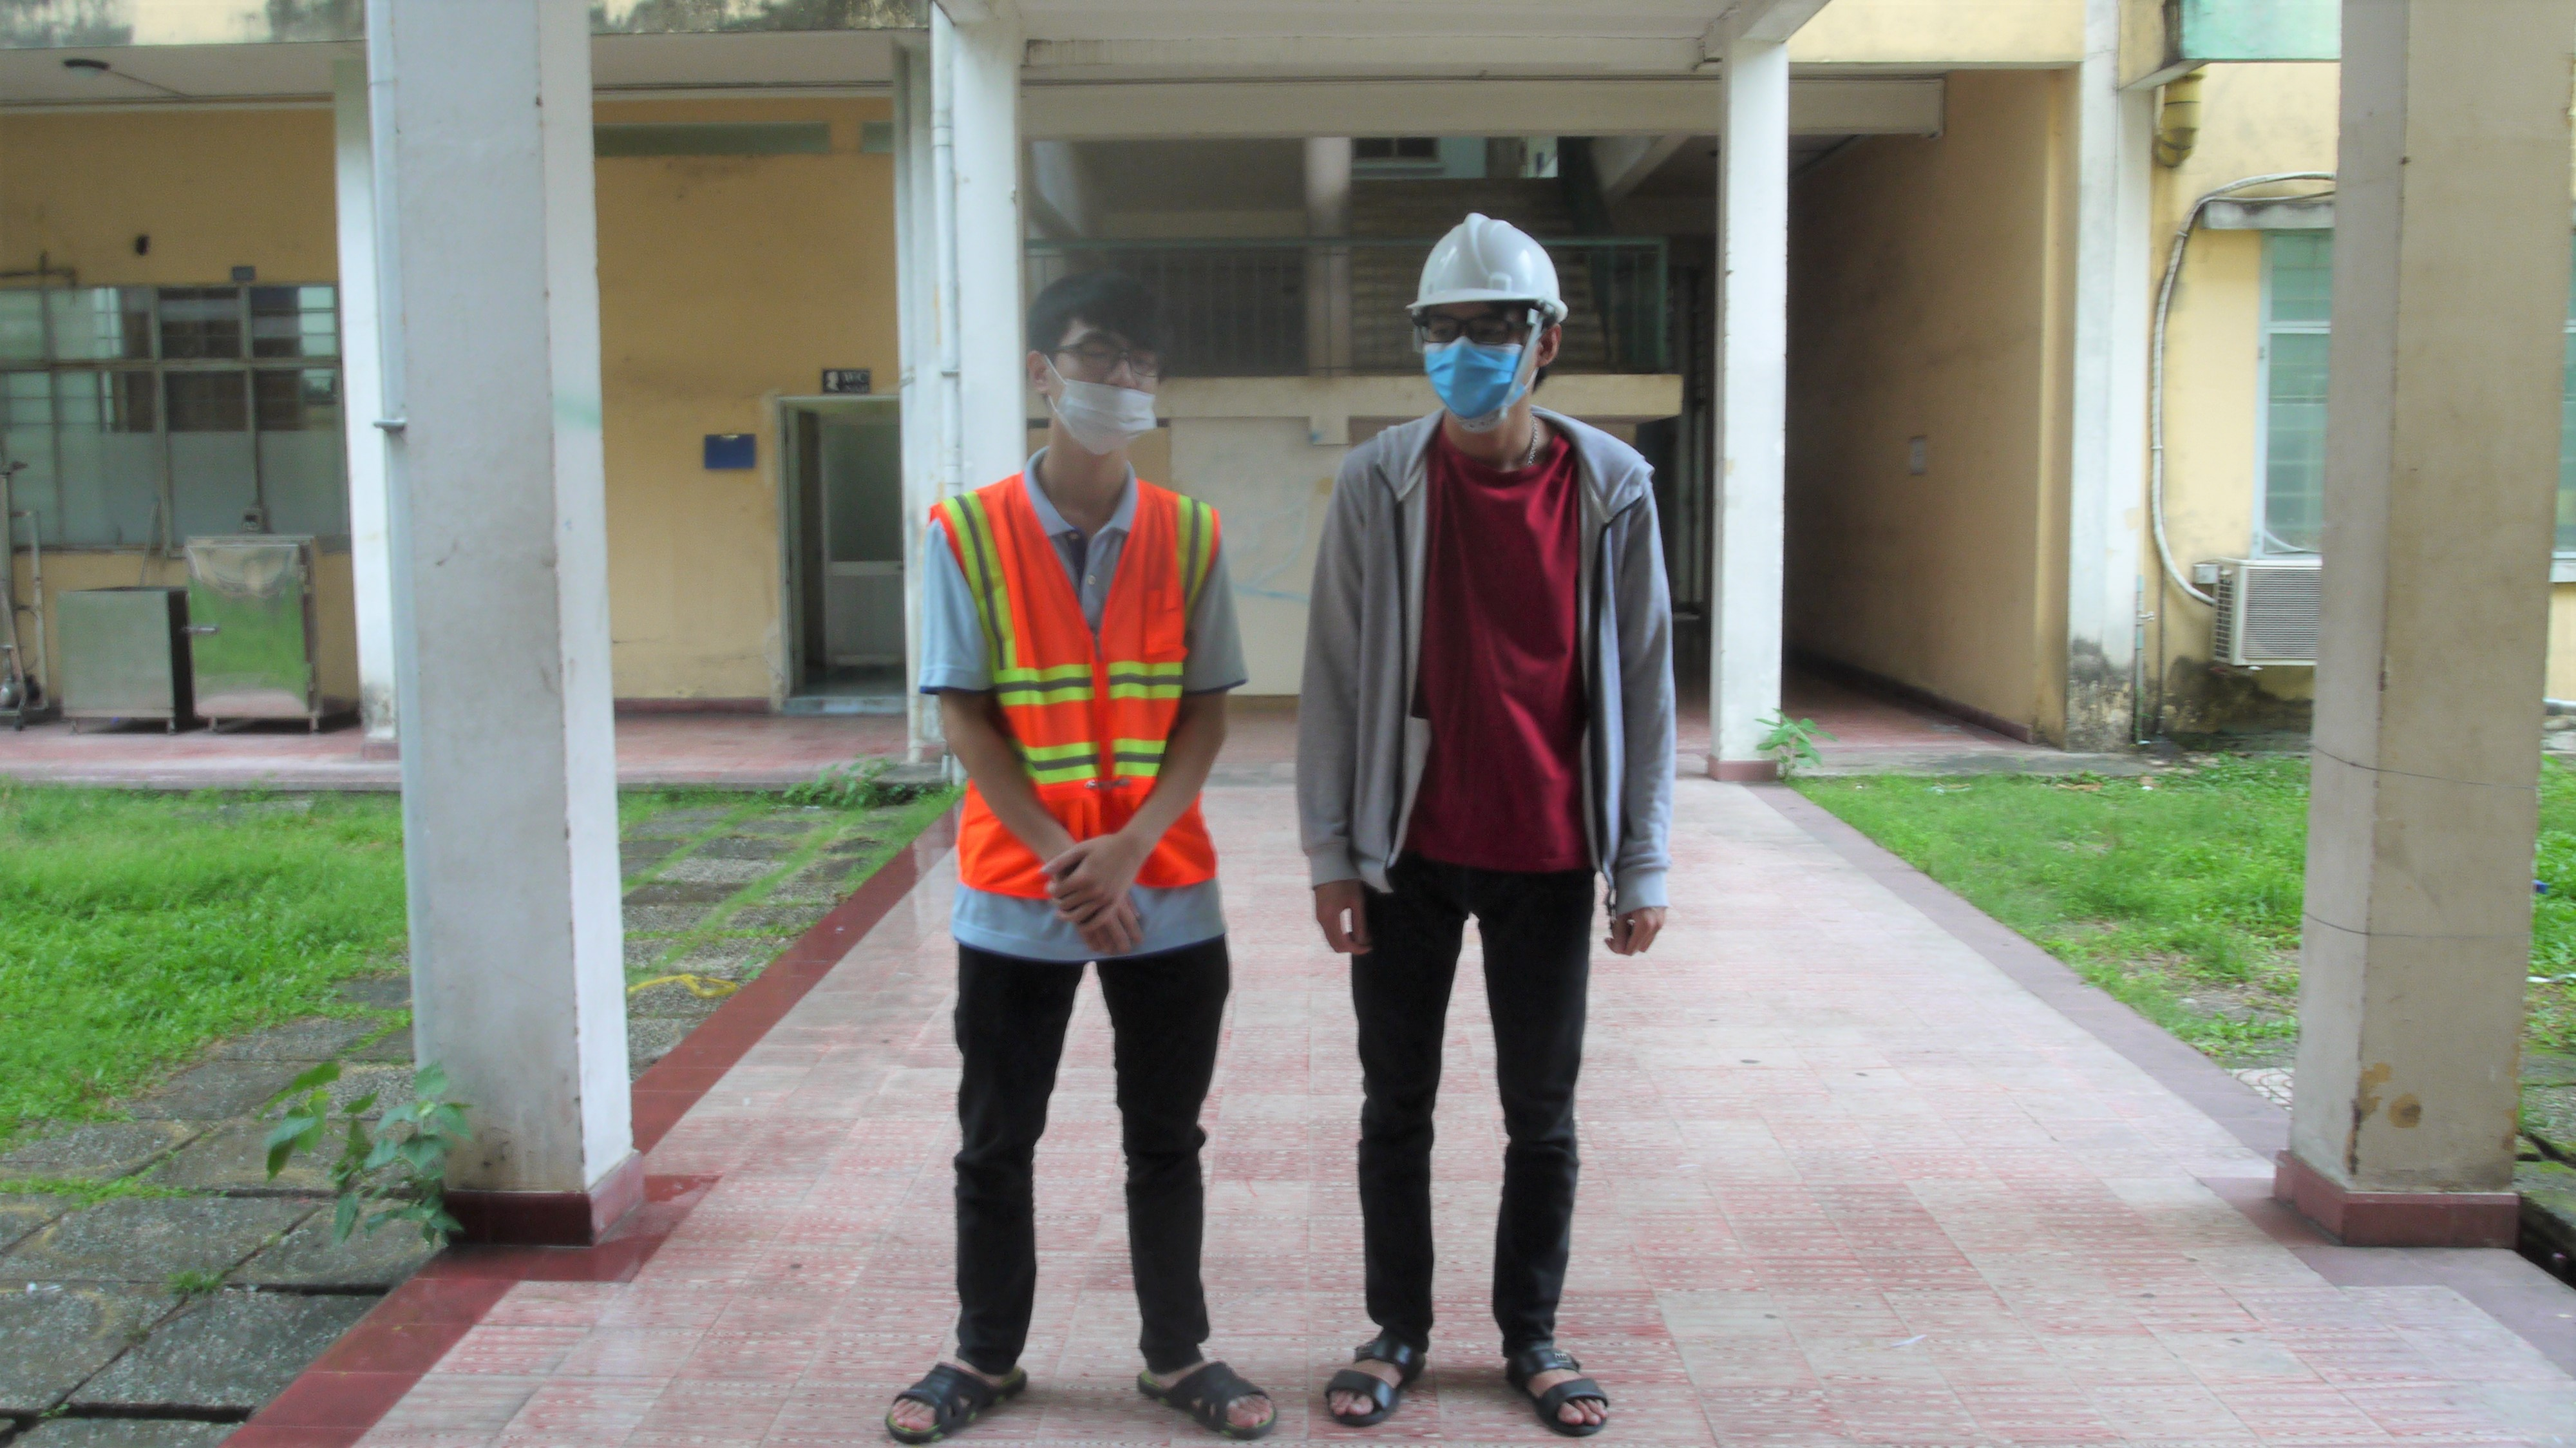
\includegraphics[width=\textwidth]{images/3m1.JPG}
\caption{The subjects stand at a distance of 3m from the camera.}
\label{fig:3m}
\end{minipage}\hfill
\begin{minipage}{0.45\textwidth}
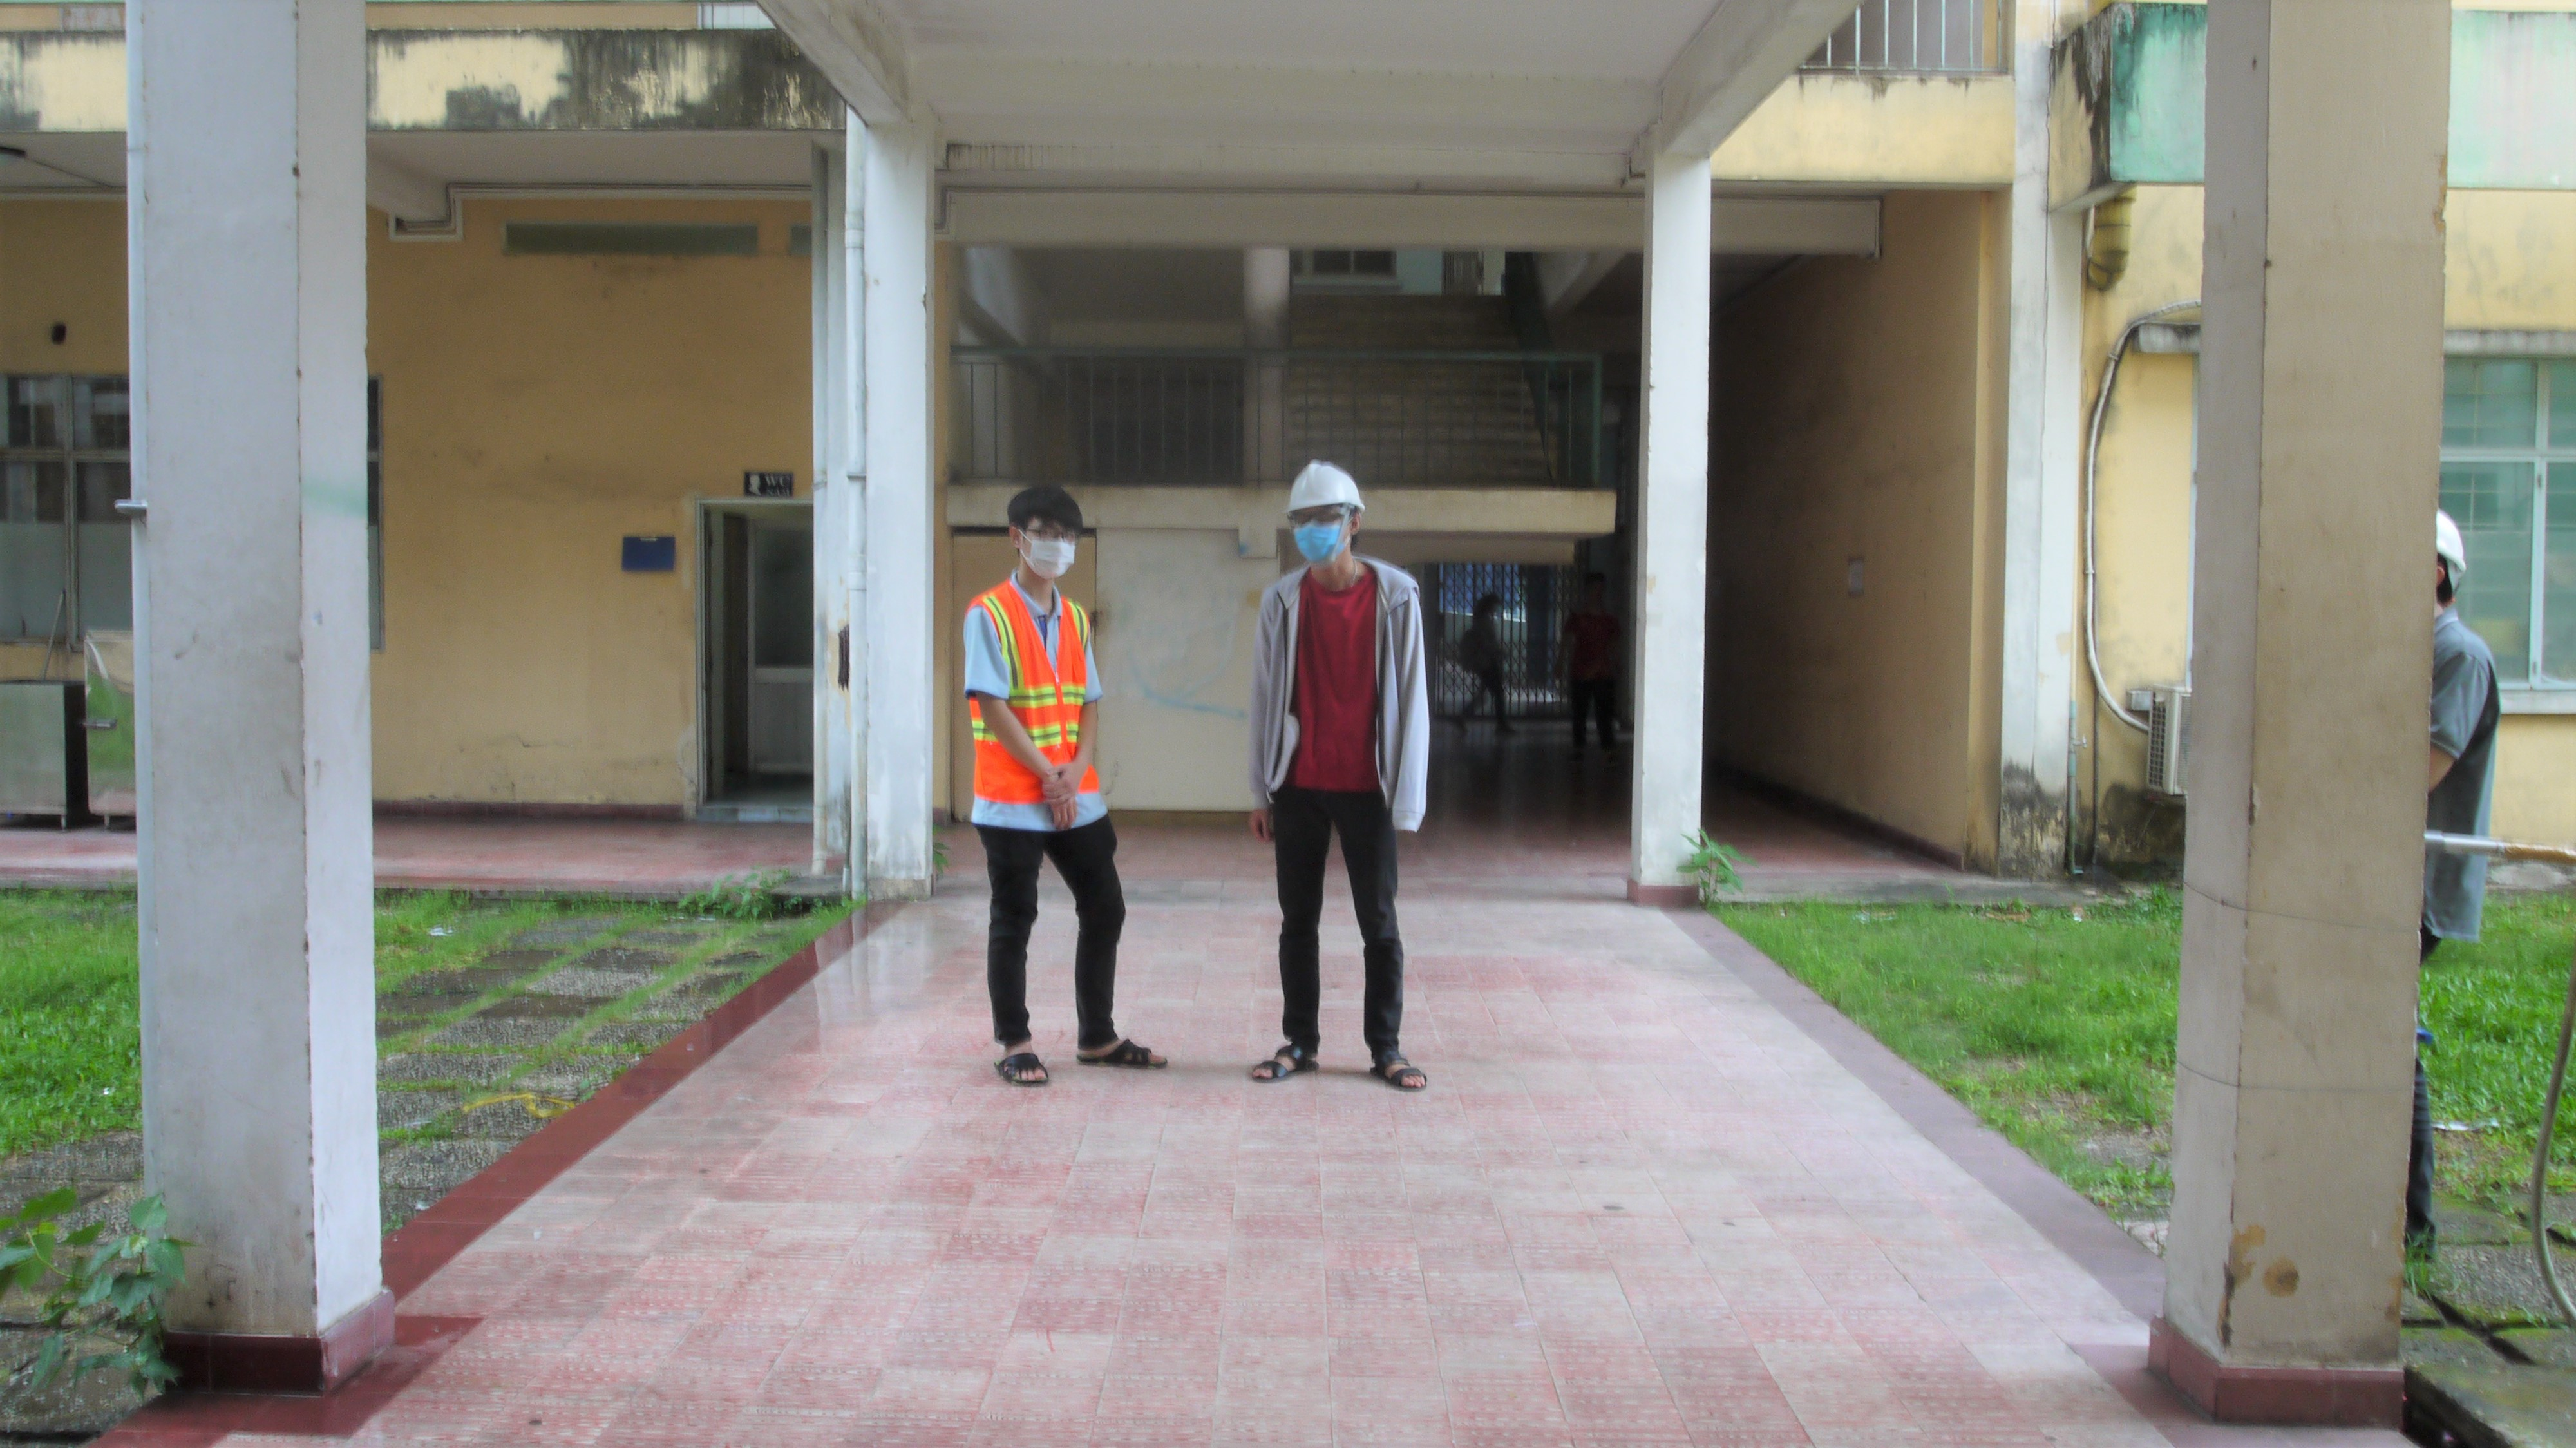
\includegraphics[width=\textwidth]{images/6m1.JPG}
\caption{The subjects stand at a distance of 6m from the camera.}
\label{fig:6m}
\end{minipage}\par
\vskip\floatsep% normal separation between figures
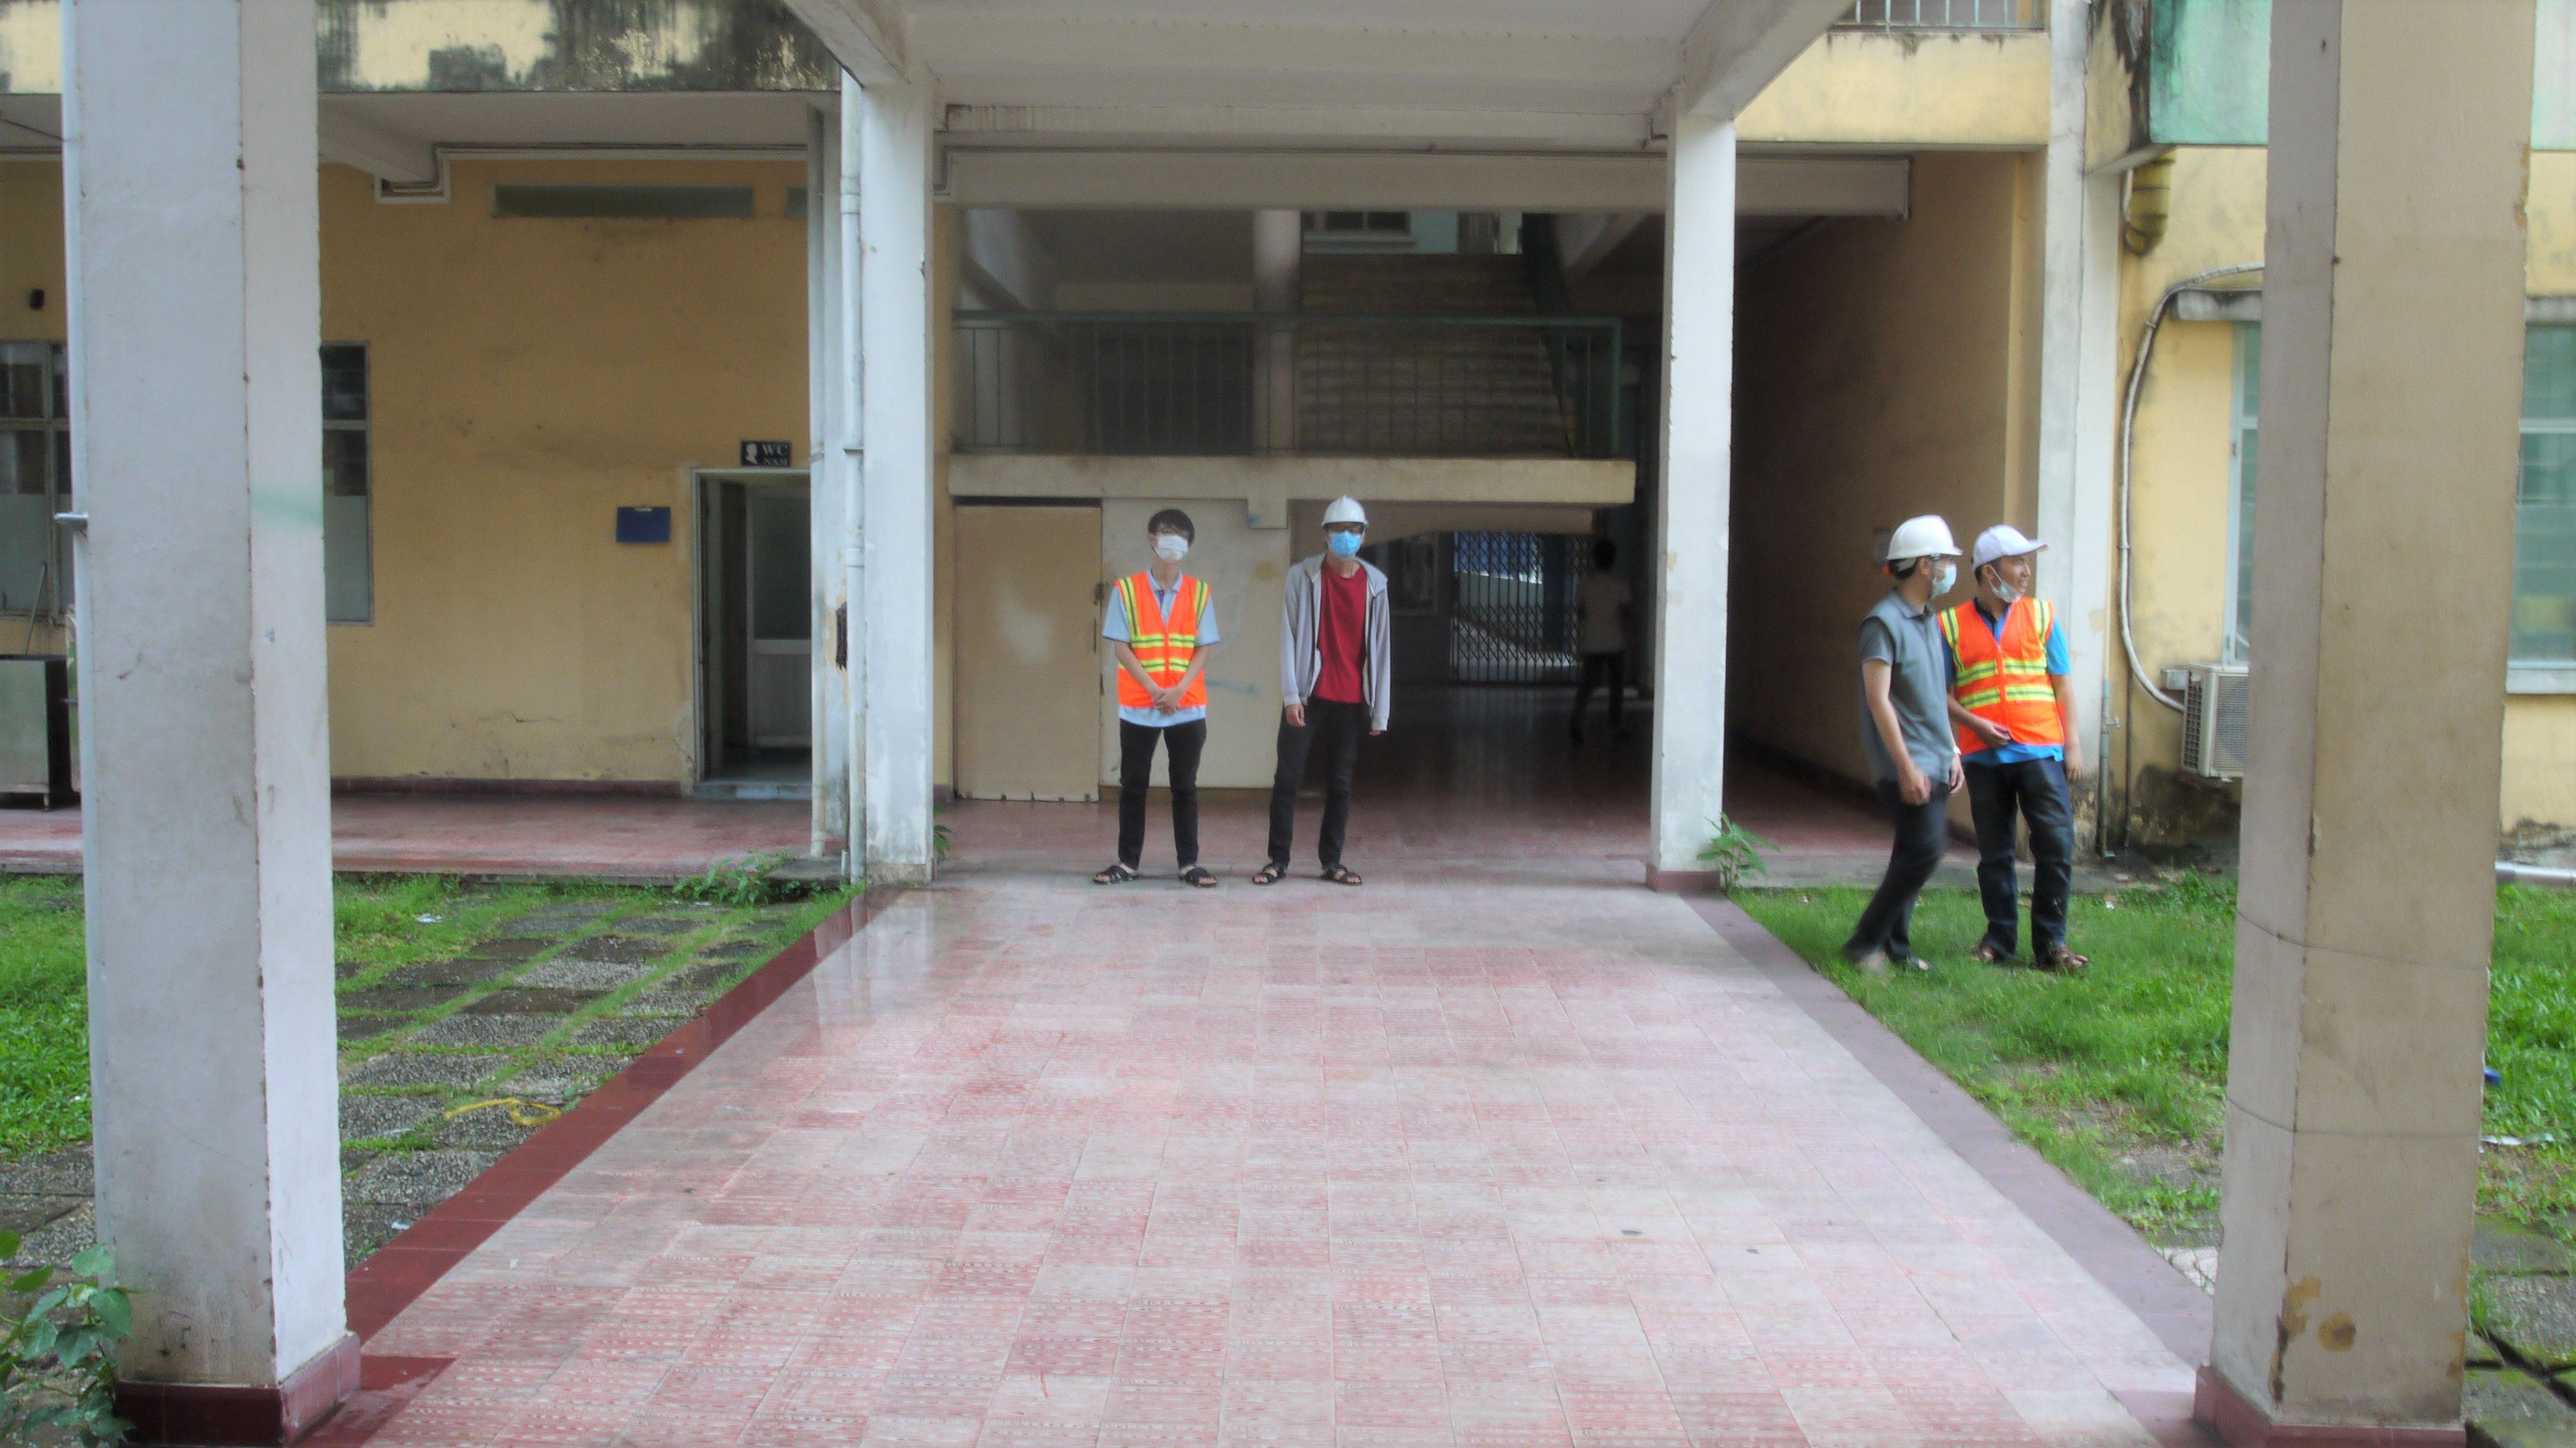
\includegraphics[width=0.45\textwidth]{images/9m1.JPG}
\caption{The subjects stand at a distance of 9m from the camera.}
\label{fig:9m}
\end{figure}
In addition, there will be a subject using a white cloth hat, similar to the white hard hat - the image \ref{fig:similar_white_hat_1} and the image \ref{fig:similar_white_hat_2} to test the ability to distinguish objects almost the same of the model.
\begin{figure}[ht]
\centering
\begin{minipage}{0.45\textwidth}
\includegraphics[width=\textwidth]{images/close1.JPG}
\caption{One subject wearing a white cloth hat - left and one subject wearing a white hard hat - right. Direct shooting angle.}
\label{fig:similar_white_hat_1}
\end{minipage}\hfill
\begin{minipage}{0.45\textwidth}
\includegraphics[width=\textwidth]{images/close2.JPG}
\caption{One subject wearing a white cloth hat - left and one subject wearing a white hard hat - right. Angle taken from the left.}
\label{fig:similar_white_hat_2}
\end{minipage}
\end{figure}

\emph{Result}: The precision graph in the figure \ref{fig:3_6_9_precision} and recalling in the figure \ref{fig:3_6_9_recall} shows that the model works best at a distance of $ 6 $ m. The precision and recall parameters of most classes at $ 6 $ m are superior to those at $ 3 $ m and $ 9 $ m. The high precision will help make the model's predictions at $ 6 $ m more accurate than at $ 3 $ m and $ 9 $ m. High recall indicates that the model is more sensitive and can detect more objects in a frame at a distance of $ 6 $ m. At class \emph{Not wearing a hardhat} there are fluctuations in performance parameters and the predicted result at the distance of $ 6 $ m is still not the best this may stem from the bounding boxes of the class \emph{Not wearing a hardhat} in the training data set has dimensions similar to the bounding boxes of objects of the same class at a distance of $ 9 $ m.
\begin{figure}[ht!]
	\centerline{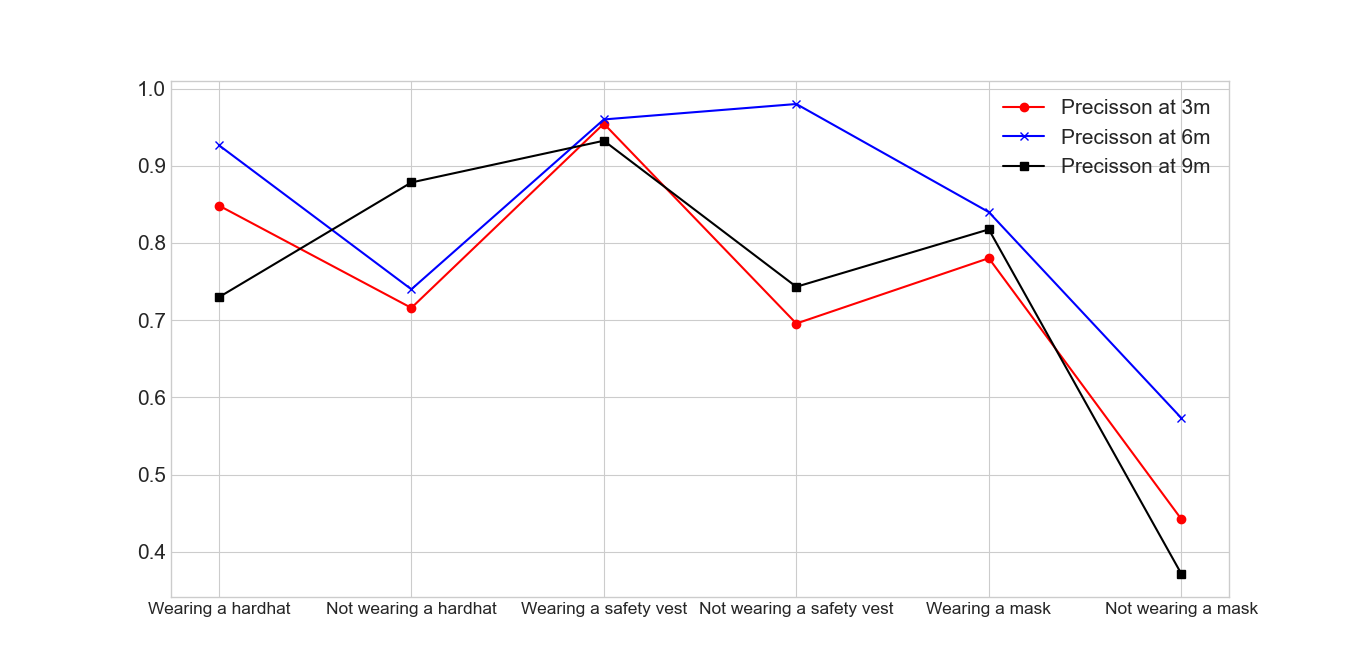
\includegraphics[scale=0.3]{images/3_6_9_precision.png}}
  	\caption{Precision of classes at distances of 3m - red, 6m - blue and 9m - black. Higher means better.}
  	\label{fig:3_6_9_precision}
\end{figure}
\begin{figure}[ht!]
	\centerline{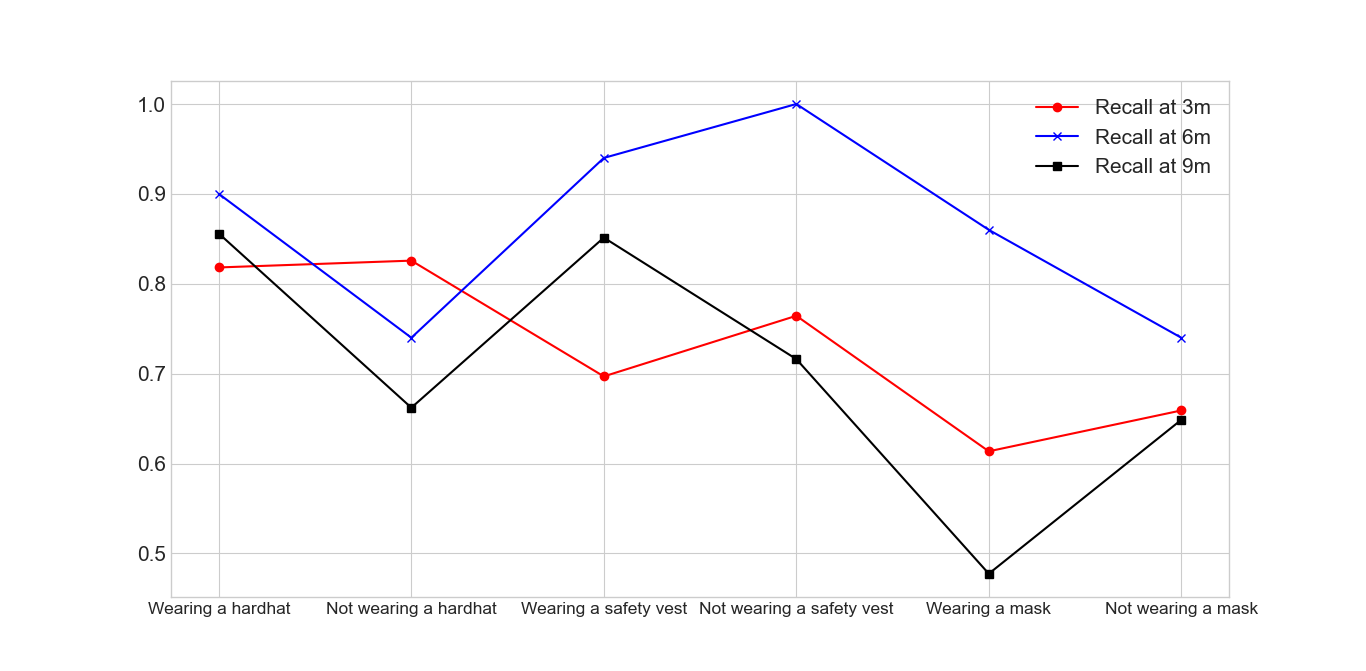
\includegraphics[scale=0.3]{images/3_6_9_recall.png}}
  	\caption{Recall of classes at distances of 3m - red, 6m - blue and 9m - black. Higher means better.}
  	\label{fig:3_6_9_recall}
\end{figure}

In addition, the model can distinguish well between white cloth hats and white protective hats at a distance of $ 3 $ m as shown in the figures \ref{fig:good_hh} and \ref{fig:good_hh_zoom}. At $ 6 $ m the model continues to be distinguished as shown in the \ref{fig:good_hh_6m} and \ref{fig:good_hh_6m_zoom}. The accuracy is reduced when the subject is away from the camera $ 9 $ m as shown in the figures \ref{fig:good_hh_9m} and \ref {fig:good_hh_9m_zoom}.
\begin{figure}[ht]
	\centerline{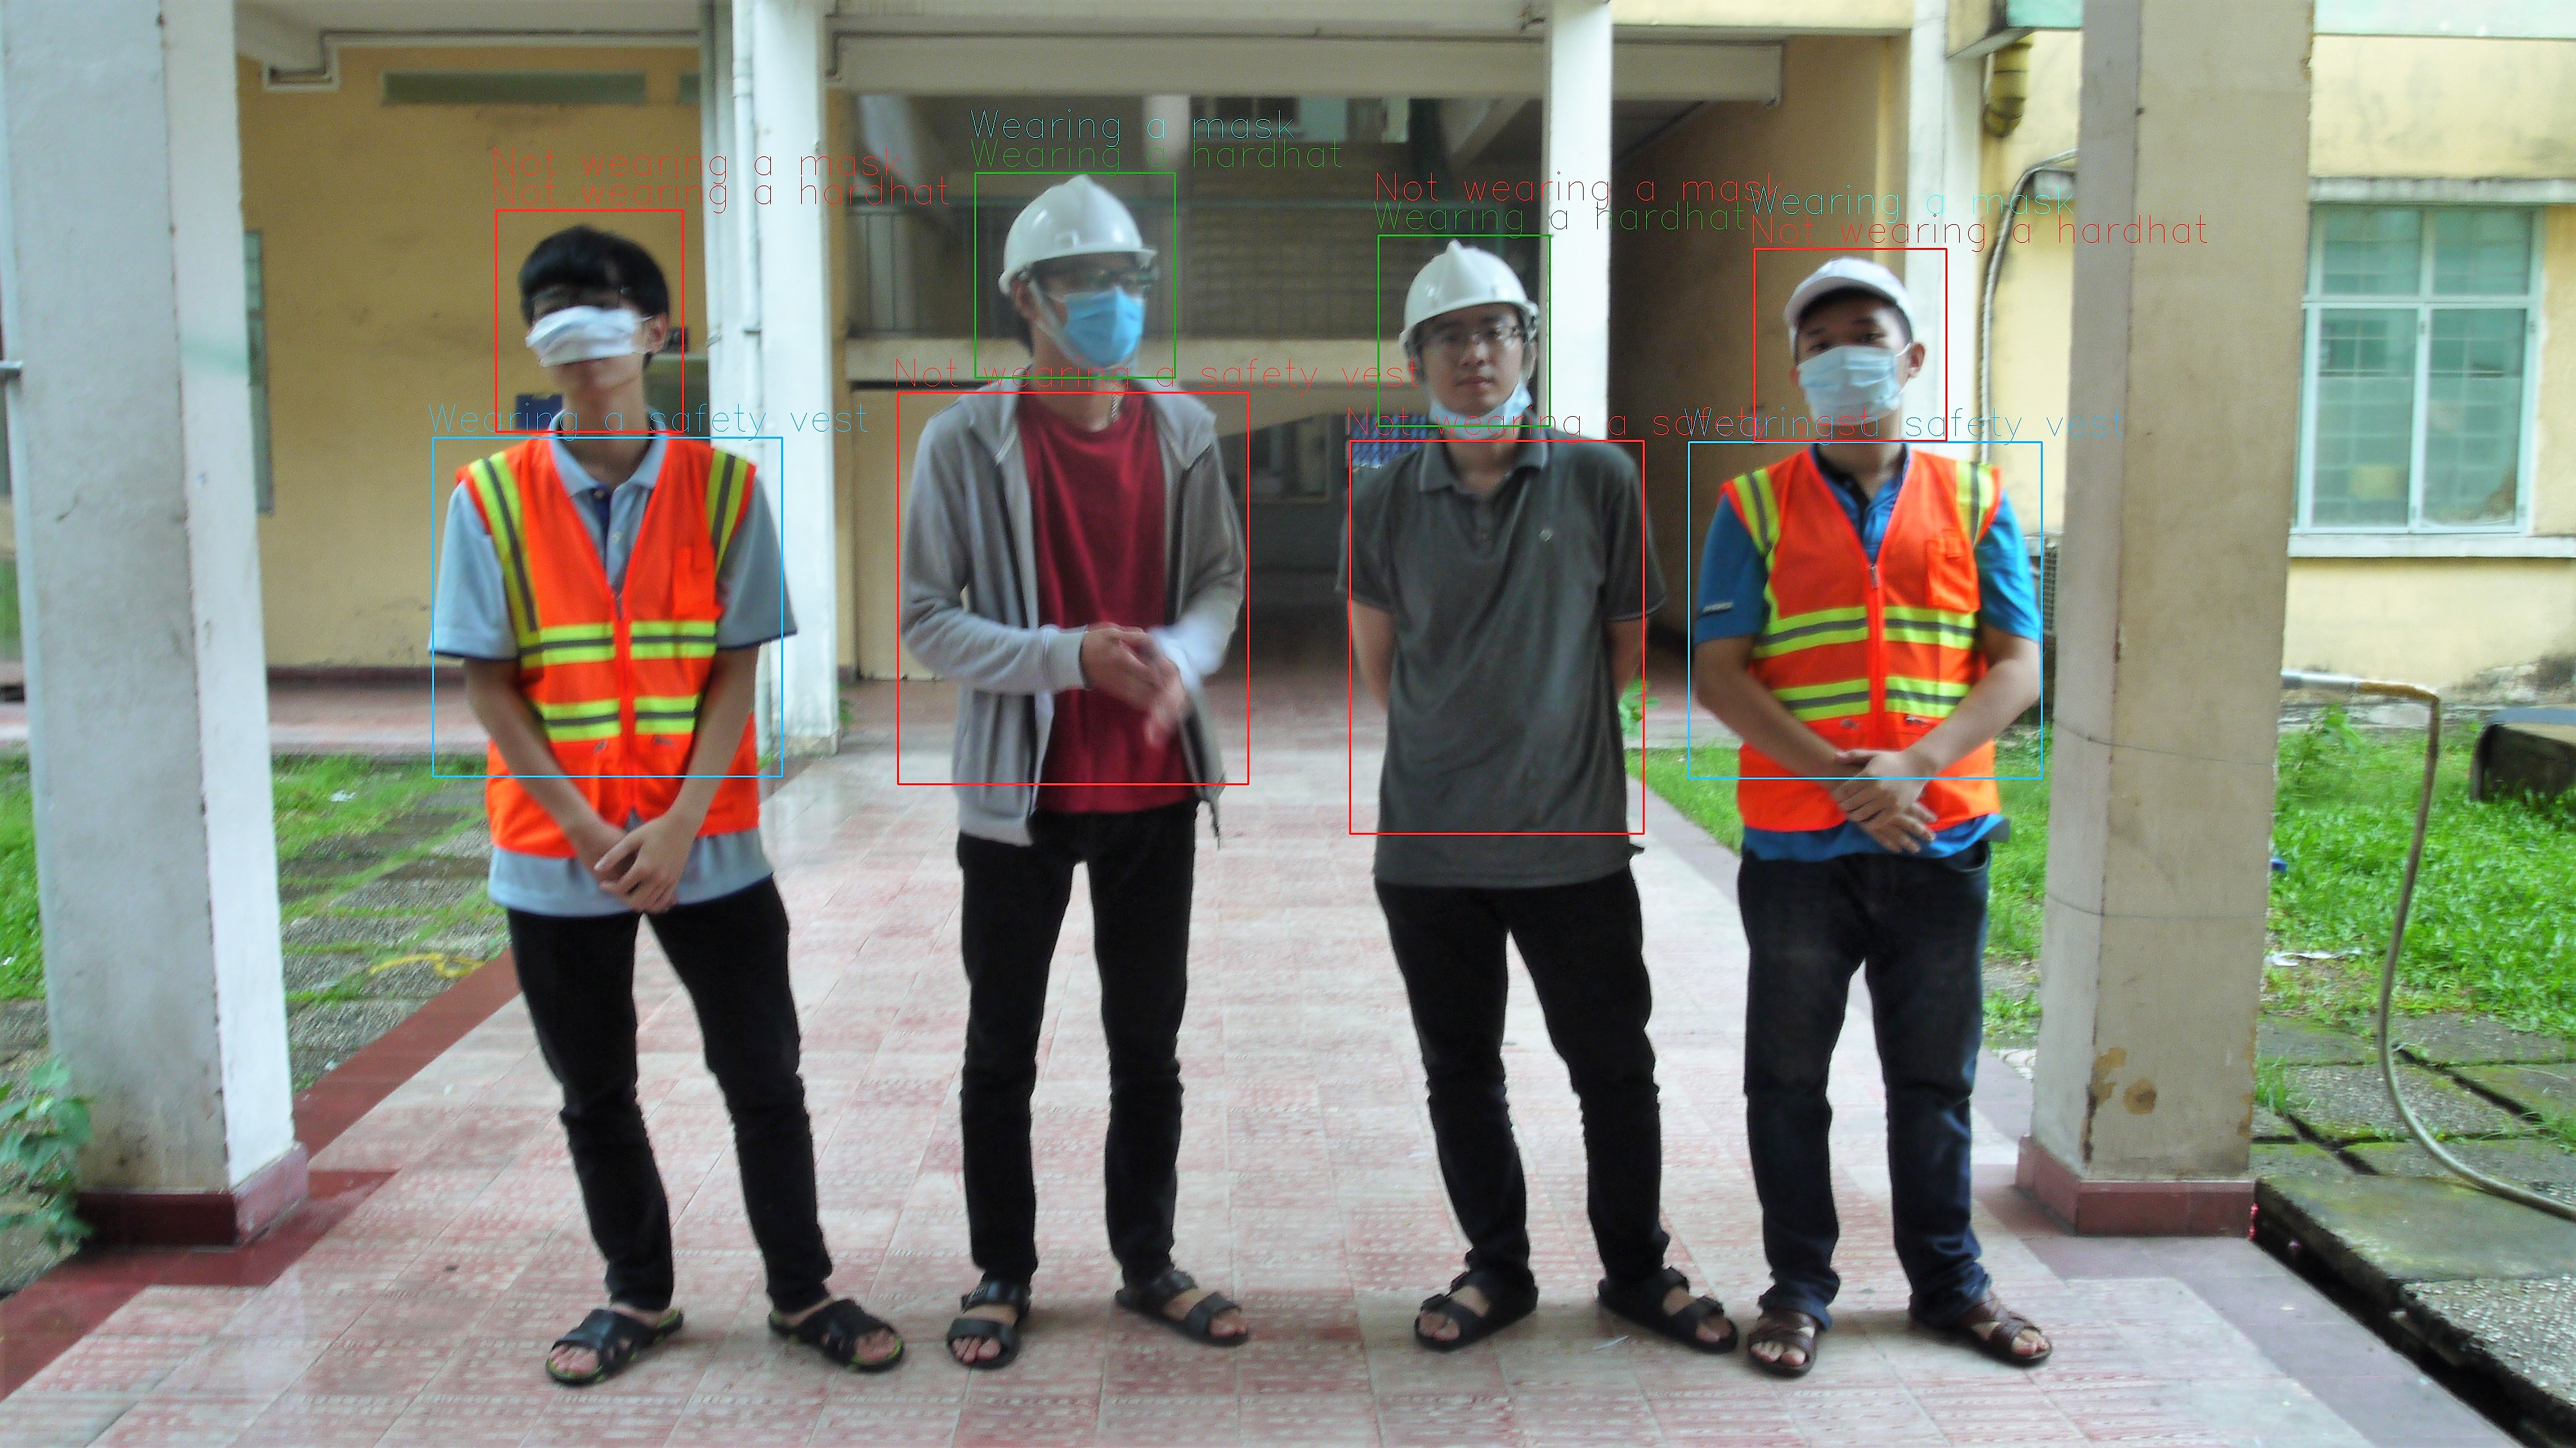
\includegraphics[scale=0.08]{images/good_hh.jpg}}
  	\caption{Prediction of the model at a distance of 3m.}
  	\label{fig:good_hh}
\end{figure}
\begin{figure}[ht]
	\centerline{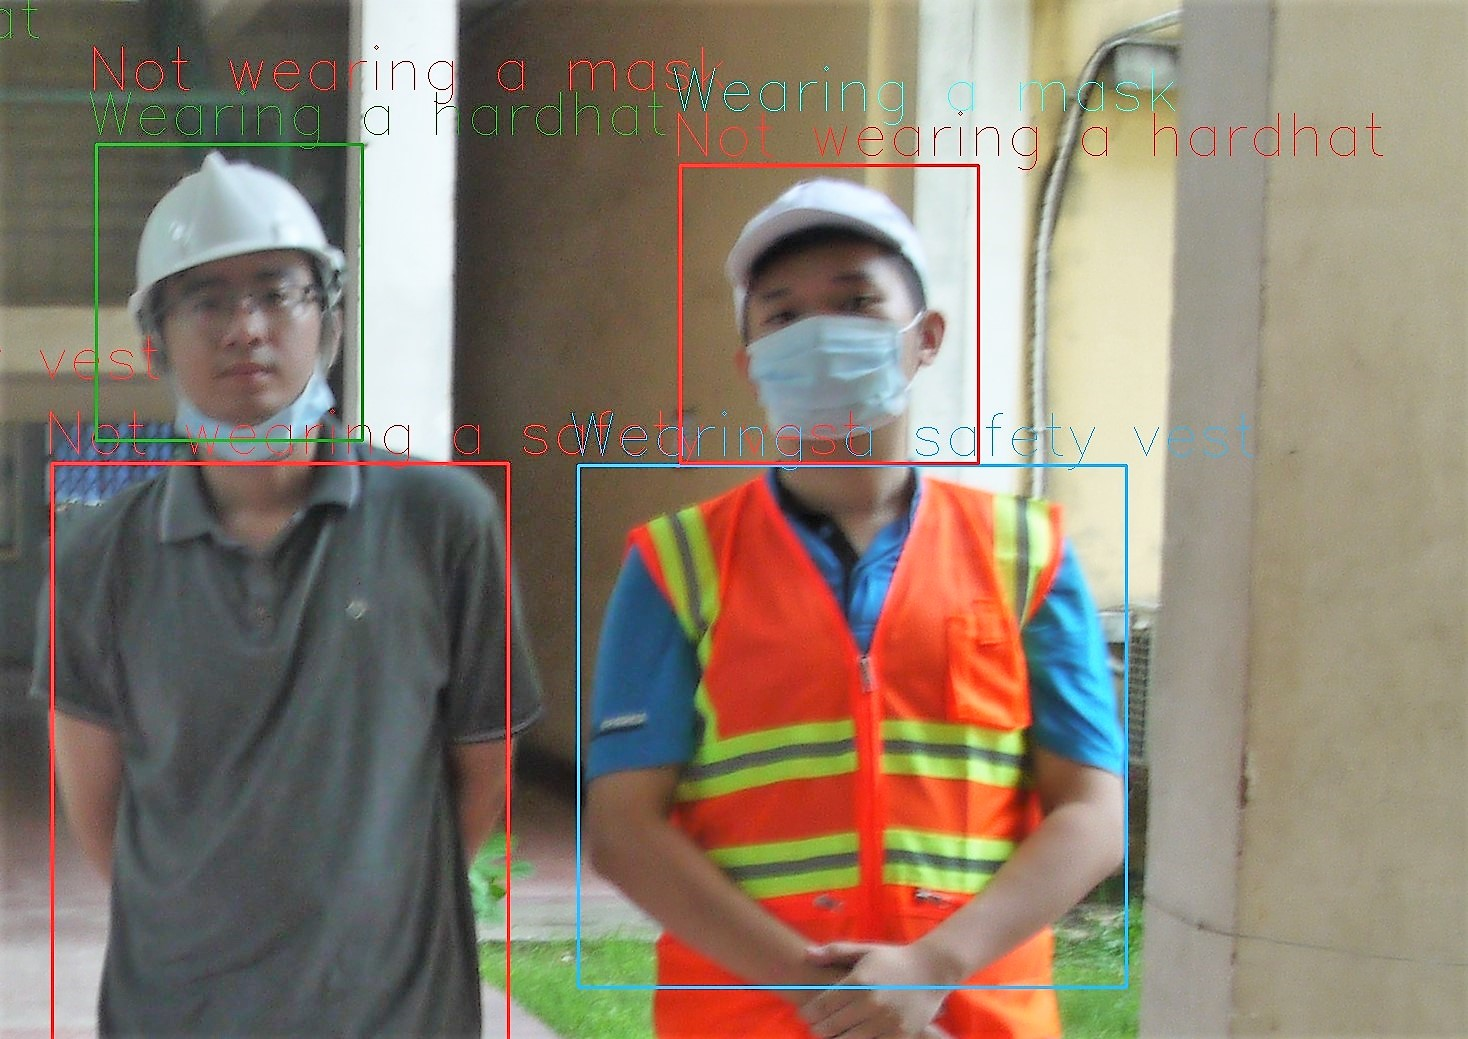
\includegraphics[scale=0.2]{images/good_hh_zoom.jpg}}
  	\caption{The model can distinguish well between white cloth hats and white hard hats at a distance of 3m.}
  	\label{fig:good_hh_zoom}
\end{figure}
\begin{figure}[ht]
	\centerline{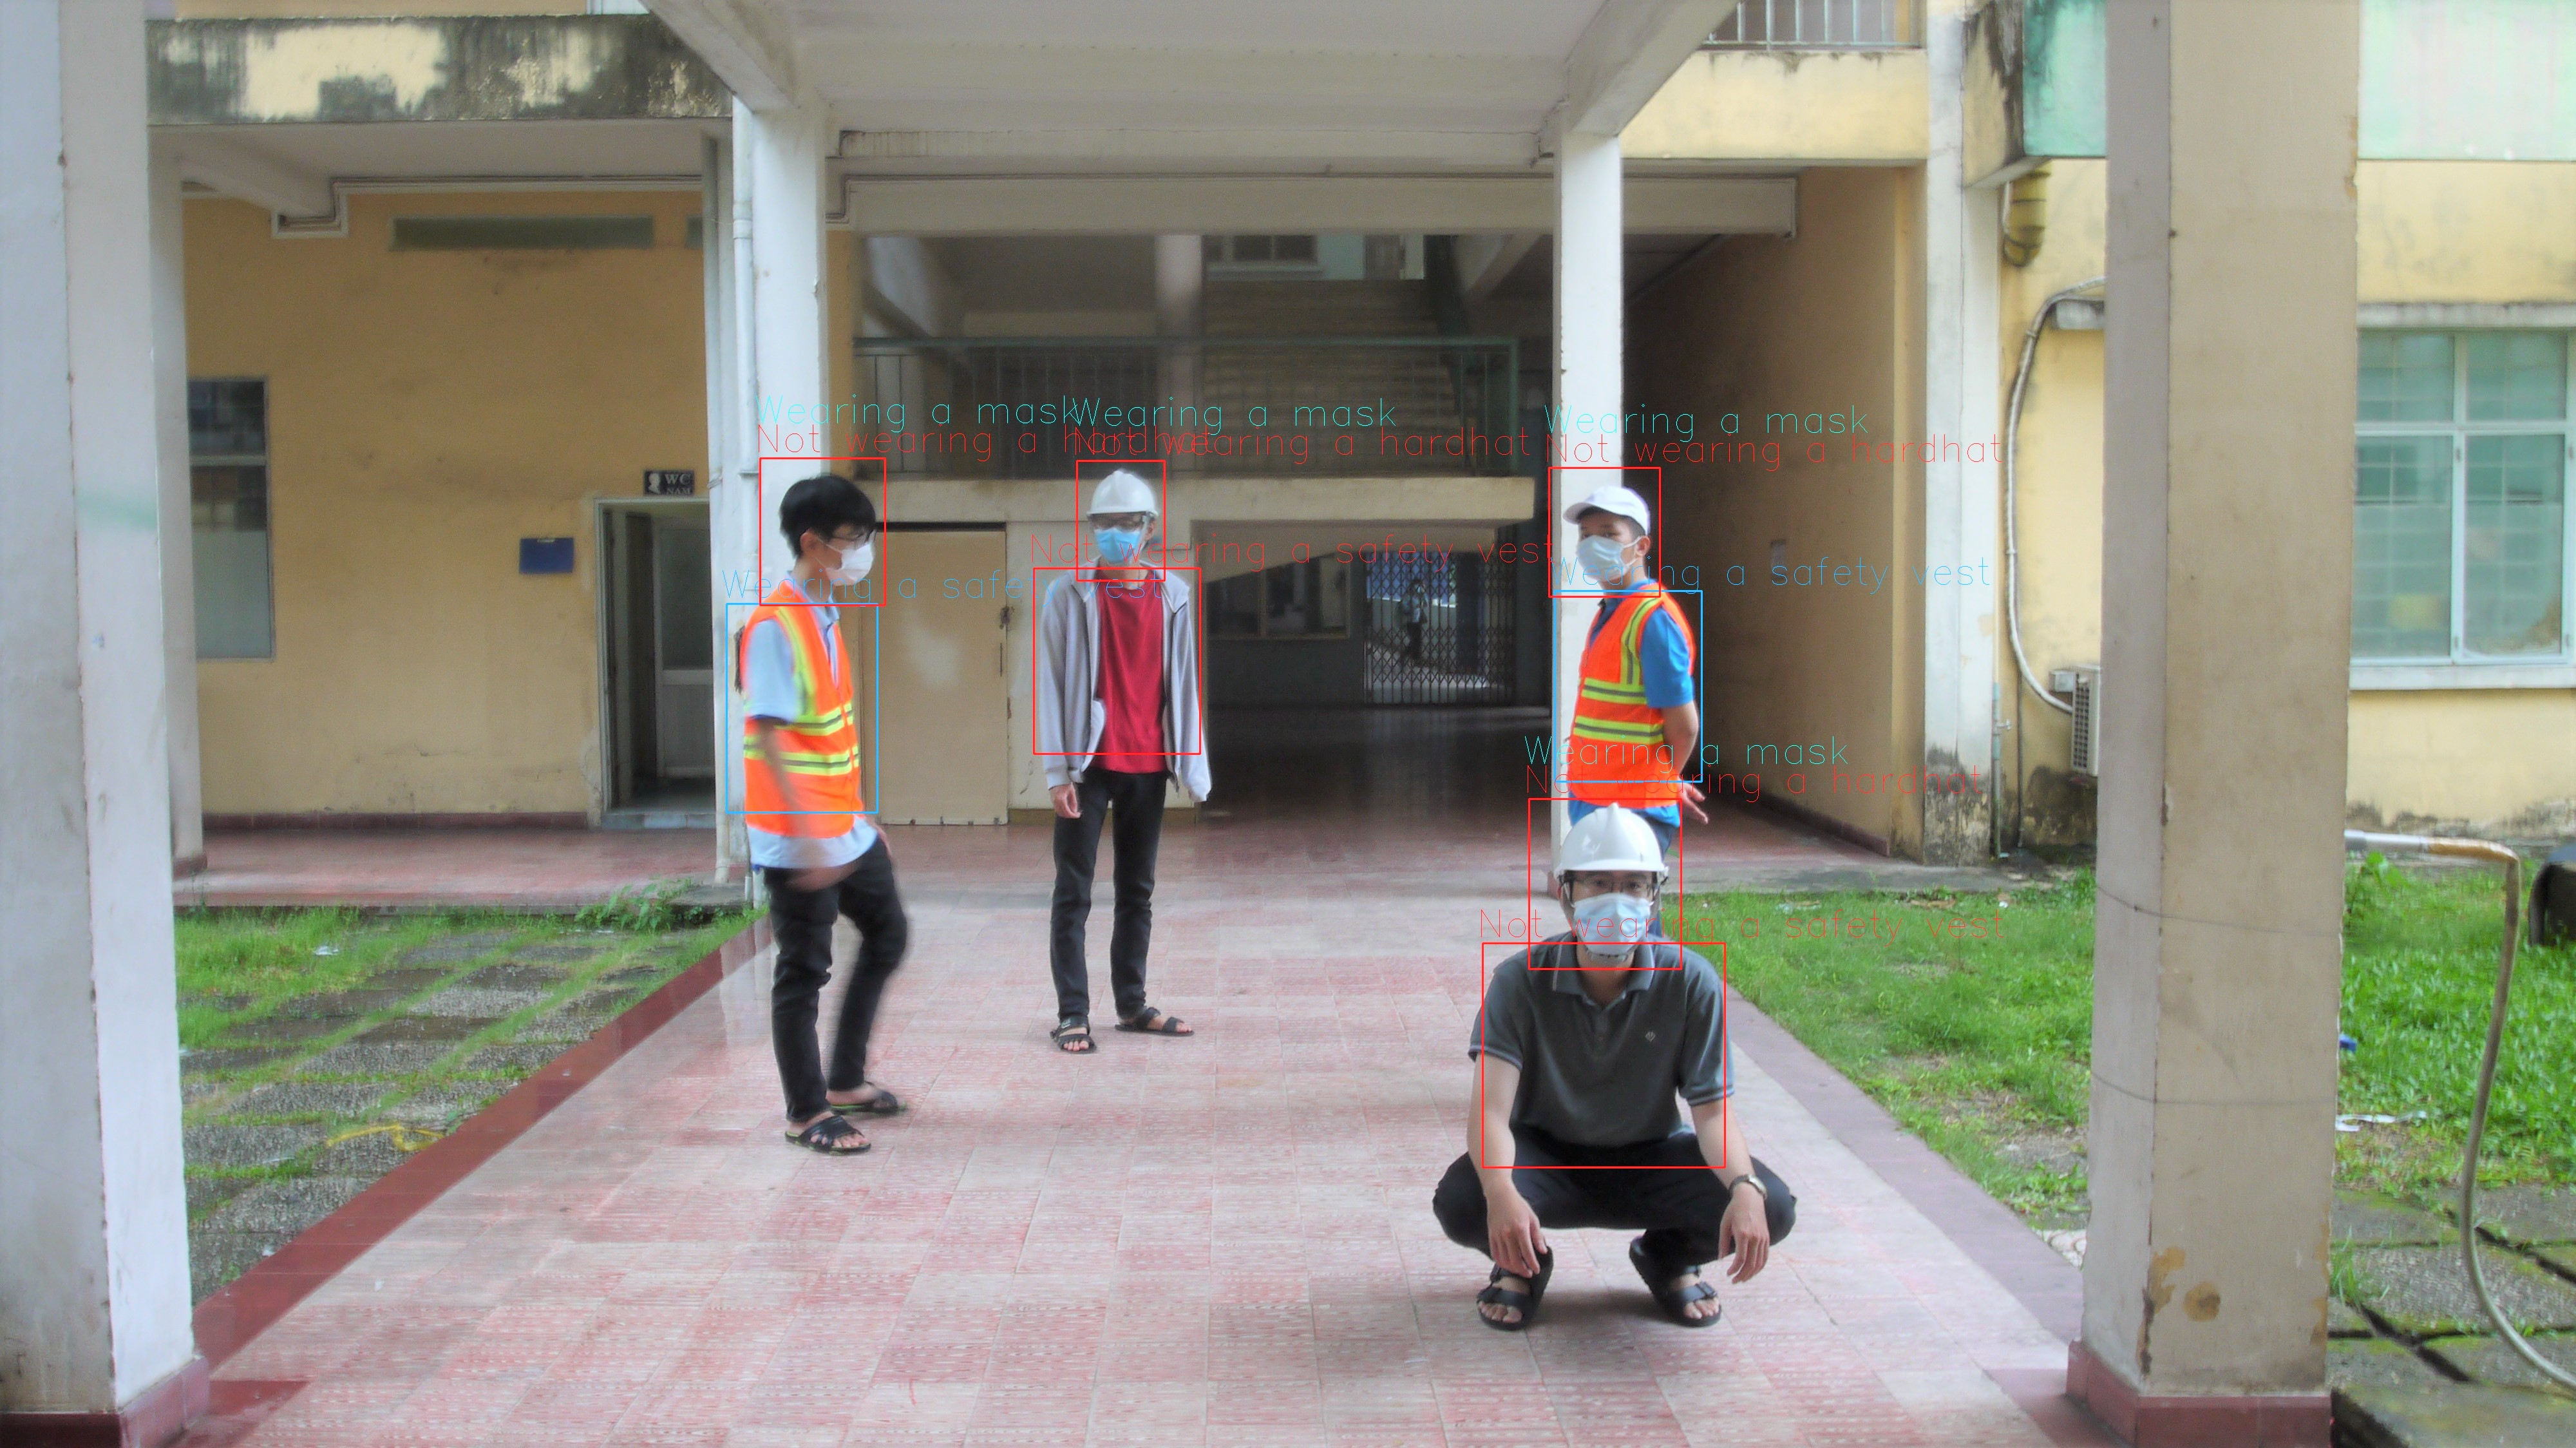
\includegraphics[scale=0.08]{images/good_hh_6m.jpg}}
  	\caption{Prediction of the model at a distance of 6m.}
  	\label{fig:good_hh_6m}
\end{figure}
\begin{figure}[ht]
	\centerline{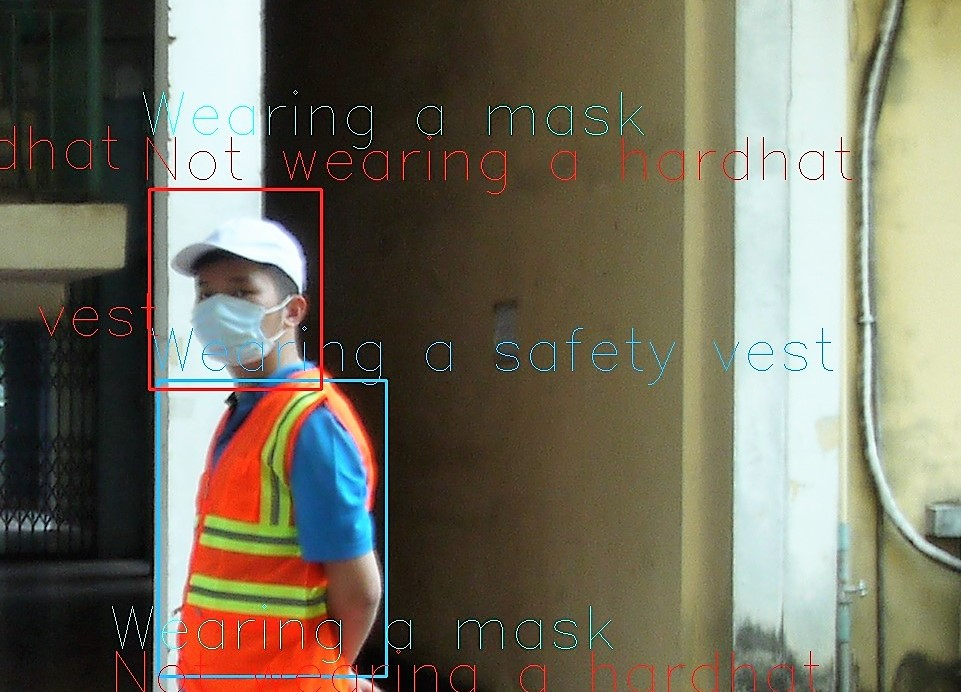
\includegraphics[scale=0.3]{images/good_hh_6m_zoom.jpg}}
  	\caption{The model can distinguish well between white cloth hats and white hard hats at a distance of 6m.}
  	\label{fig:good_hh_6m_zoom}
\end{figure}
\begin{figure}[ht]
	\centerline{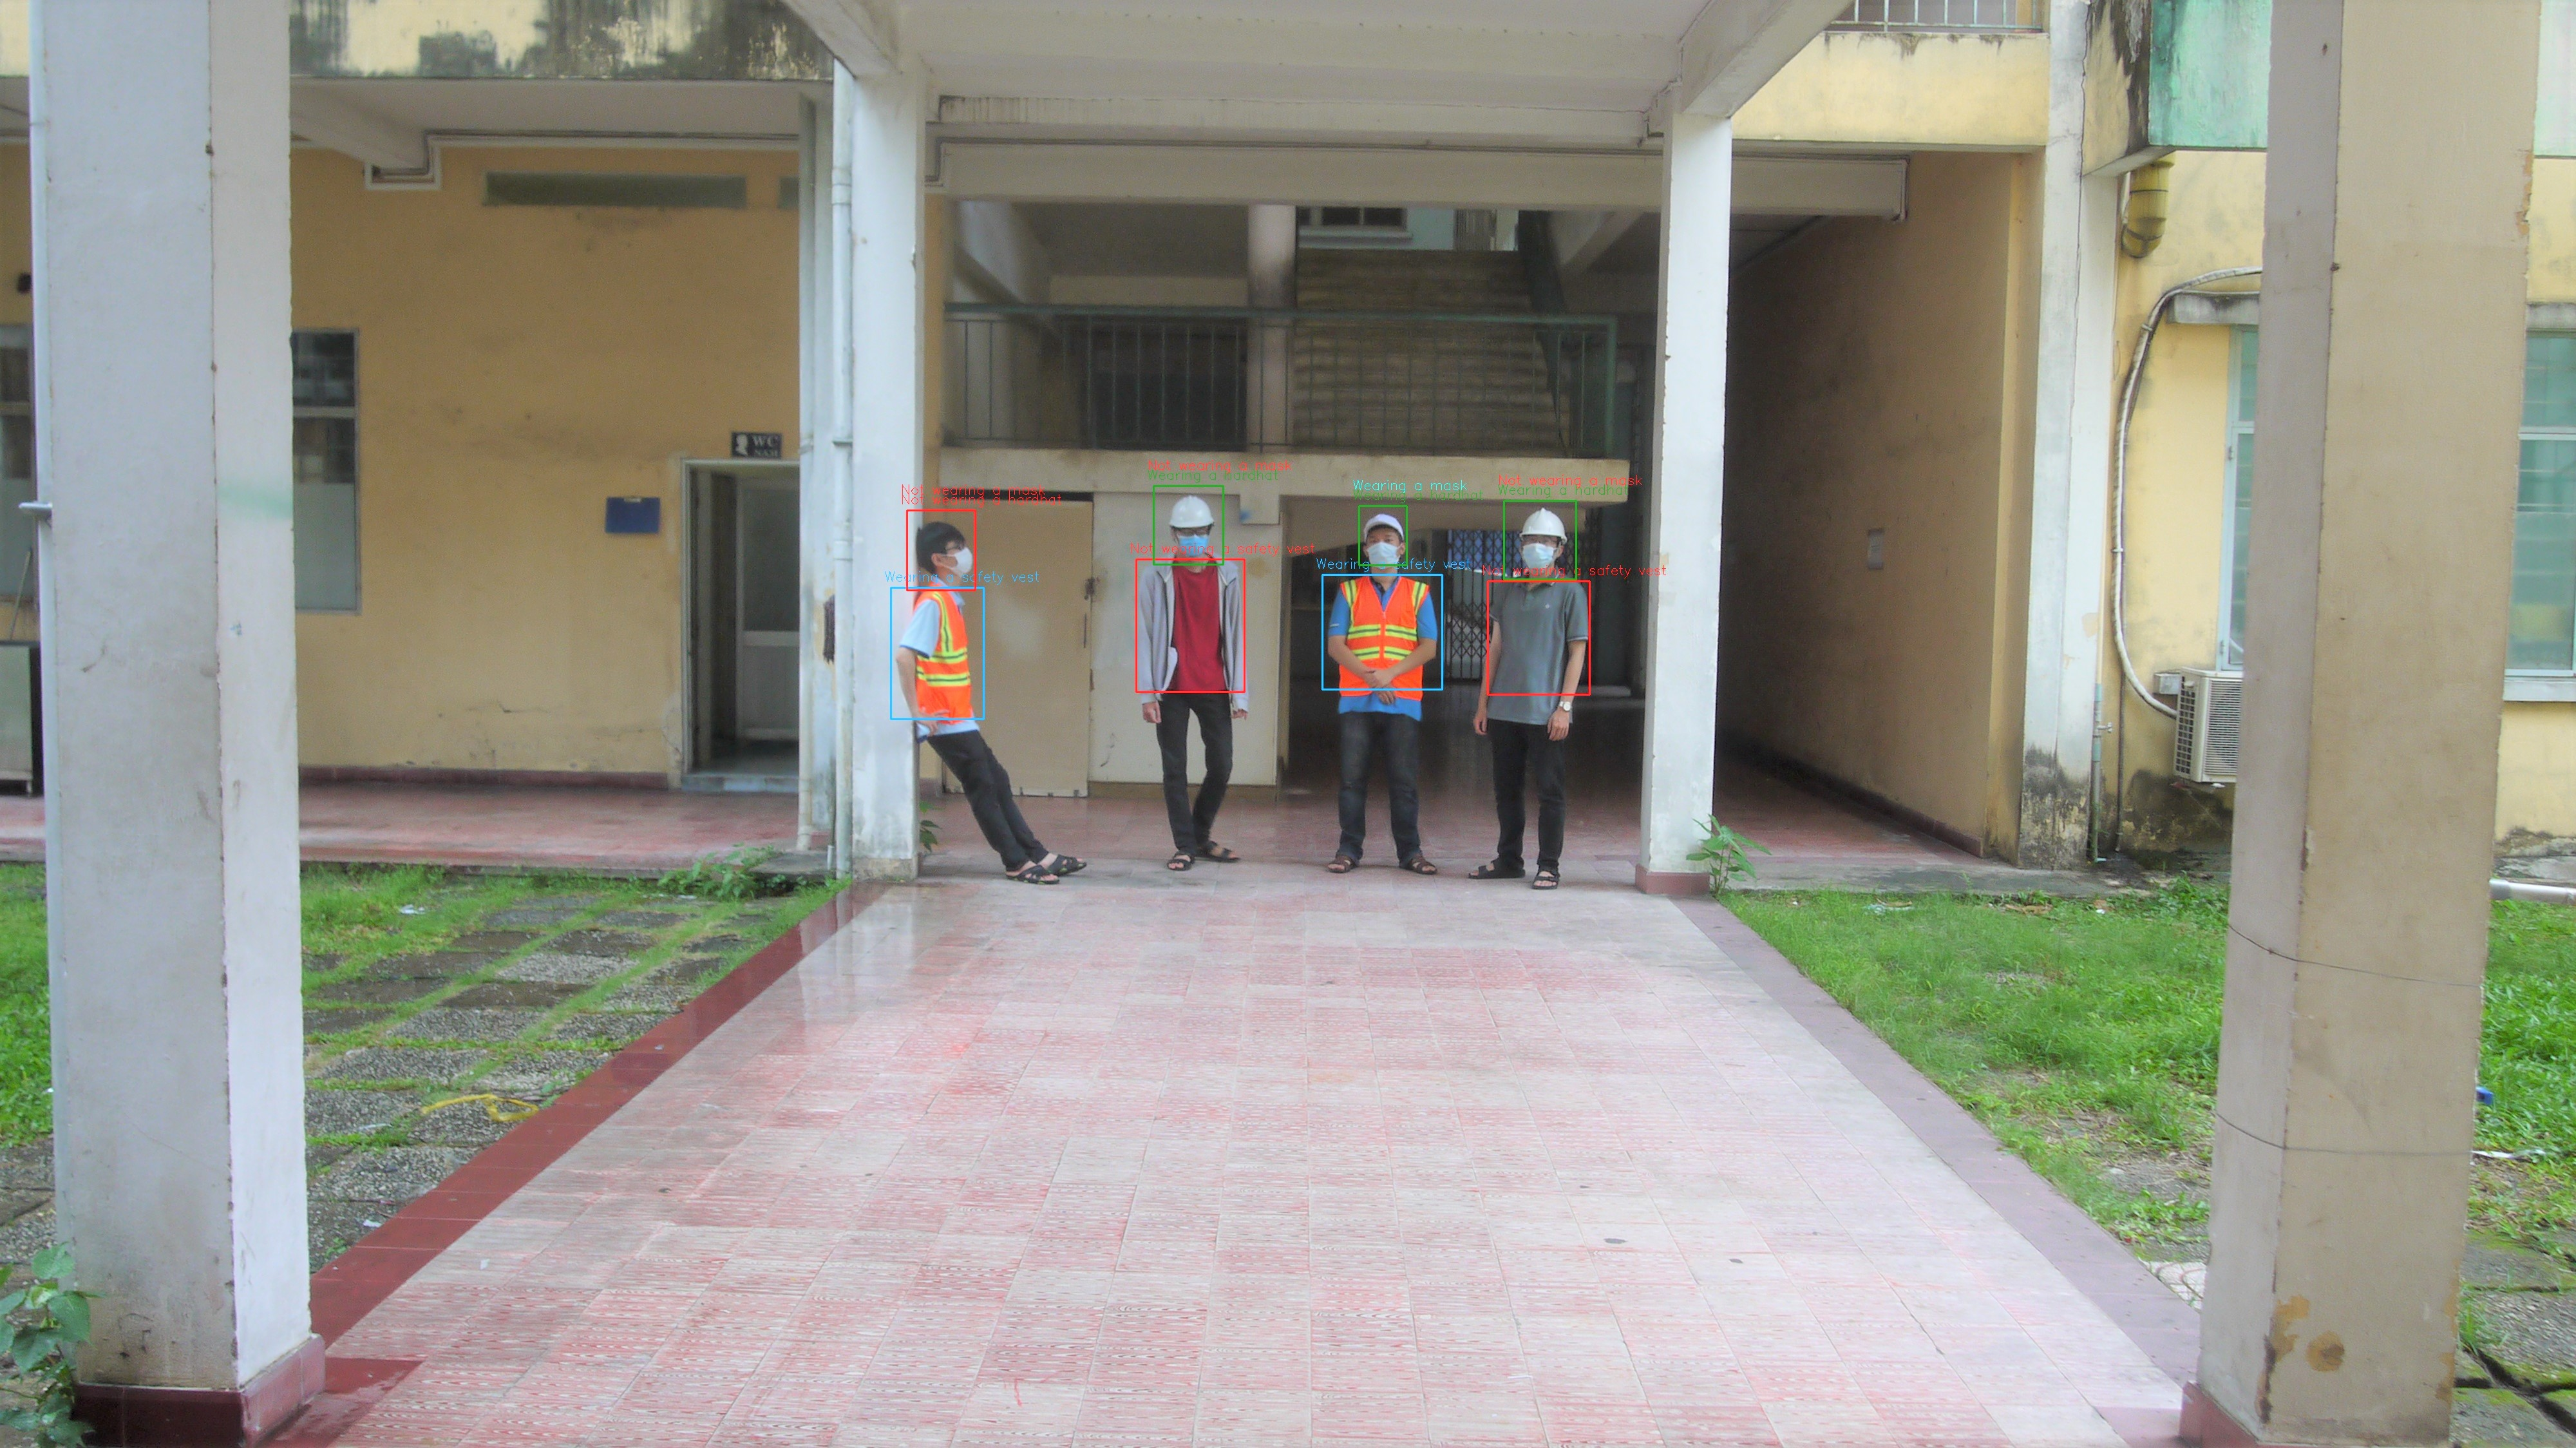
\includegraphics[scale=0.08]{images/bad_hh_9m.jpg}}
  	\caption{Prediction of the model at a distance of 9m.}
  	\label{fig:good_hh_9m}
\end{figure}
\begin{figure}[ht]
	\centerline{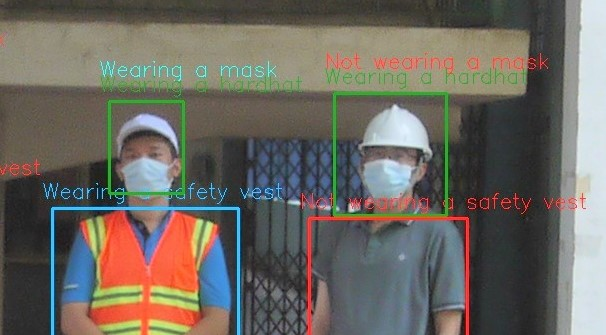
\includegraphics[scale=0.4]{images/bad_hh_9m_zoom.jpg}}
  	\caption{The model cannot distinguish well between white cloth hats and white hard hats at a distance of 9m.}
  	\label{fig:good_hh_9m_zoom}
\end{figure}

\subsubsection{Testing the model's ability to identify with cases of improper use of protective equipment}
The use of protective equipment in the wrong way is as dangerous as the absence of protective equipment, so it is not only necessary to distinguish between using or not, the model must also be able to distinguish between using. Correct and wrong use of protective equipment. In this case, the subject will wear the wrong mask or the wrong reflective vest to check the identification of the model.

\emph{Case 1}: Wearing a mask incorrectly will be done through two cases, one is to wear a mask with nose out - figure \ref{fig:bad_mask_nose}, two is to wear a mask with mouth out - figure \ref{fig:bad_mask_mouth}. The predicted results are shown in the figure at a distance of $ 3 $m.
\begin{figure}[ht]
	\centerline{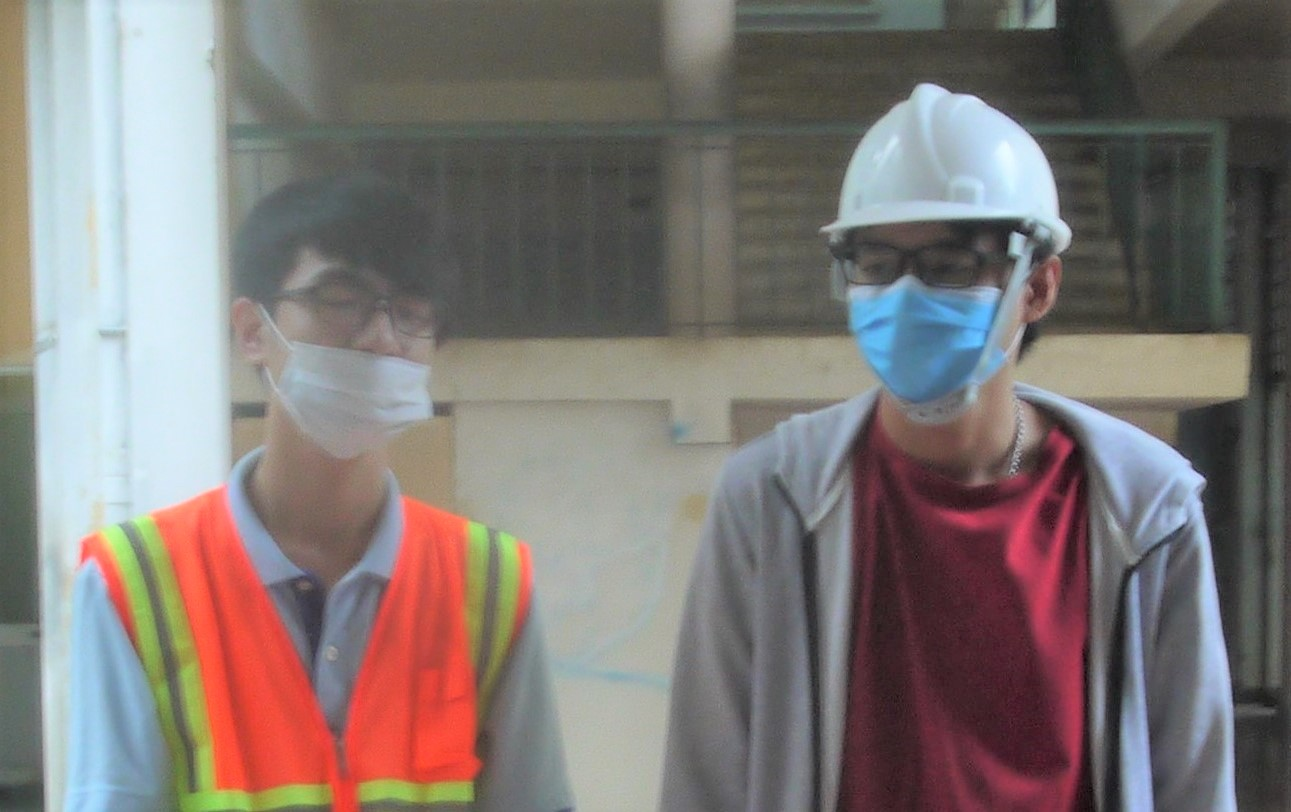
\includegraphics[scale=0.3]{images/bad_mask_nose.jpg}}
  	\caption{The subject (left) wears a mask that does not cover his/her nose at a distance of 3m.}
  	\label{fig:bad_mask_nose}
\end{figure}
\begin{figure}[ht]
	\centerline{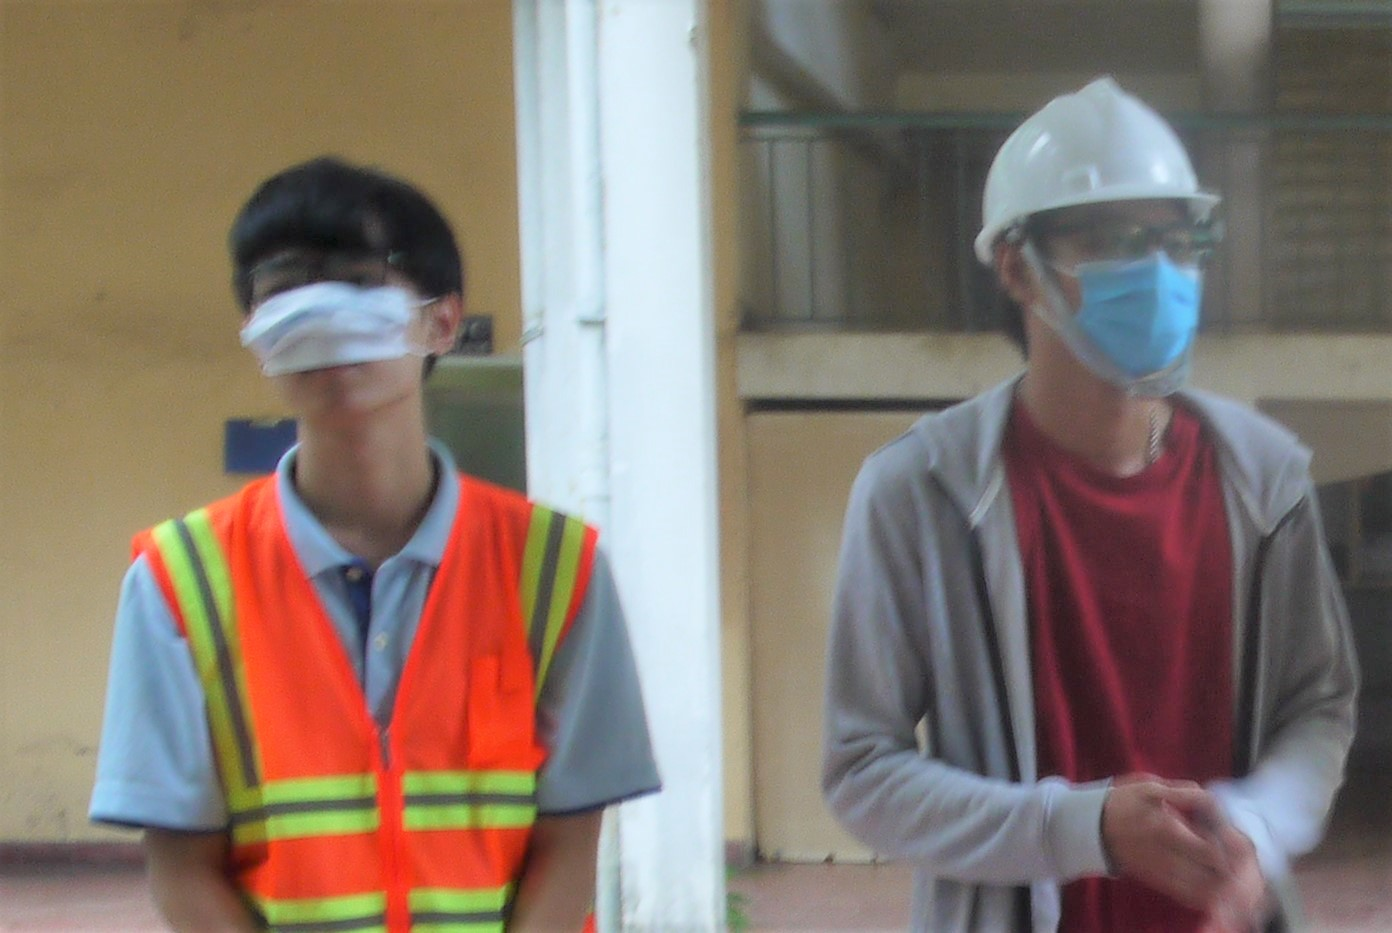
\includegraphics[scale=0.3]{images/bad_mask_mouth.jpg}}
  	\caption{The subject (left) wears a mask that does not cover his/her mouth at a distance of 3m.}
  	\label{fig:bad_mask_mouth}
\end{figure}
\emph{Result}: The model could not distinguish the case of wearing a wrong mask when the subject wearing the mask with nose out - figure \ref{fig:bad_mask_nose_pred}. The model can distinguish well in case of wearing a wrong mask when the subject is wearing an open mouth mask - figure \ref{fig:bad_mask_mouth_pred}.
\begin{figure}[ht]
	\centerline{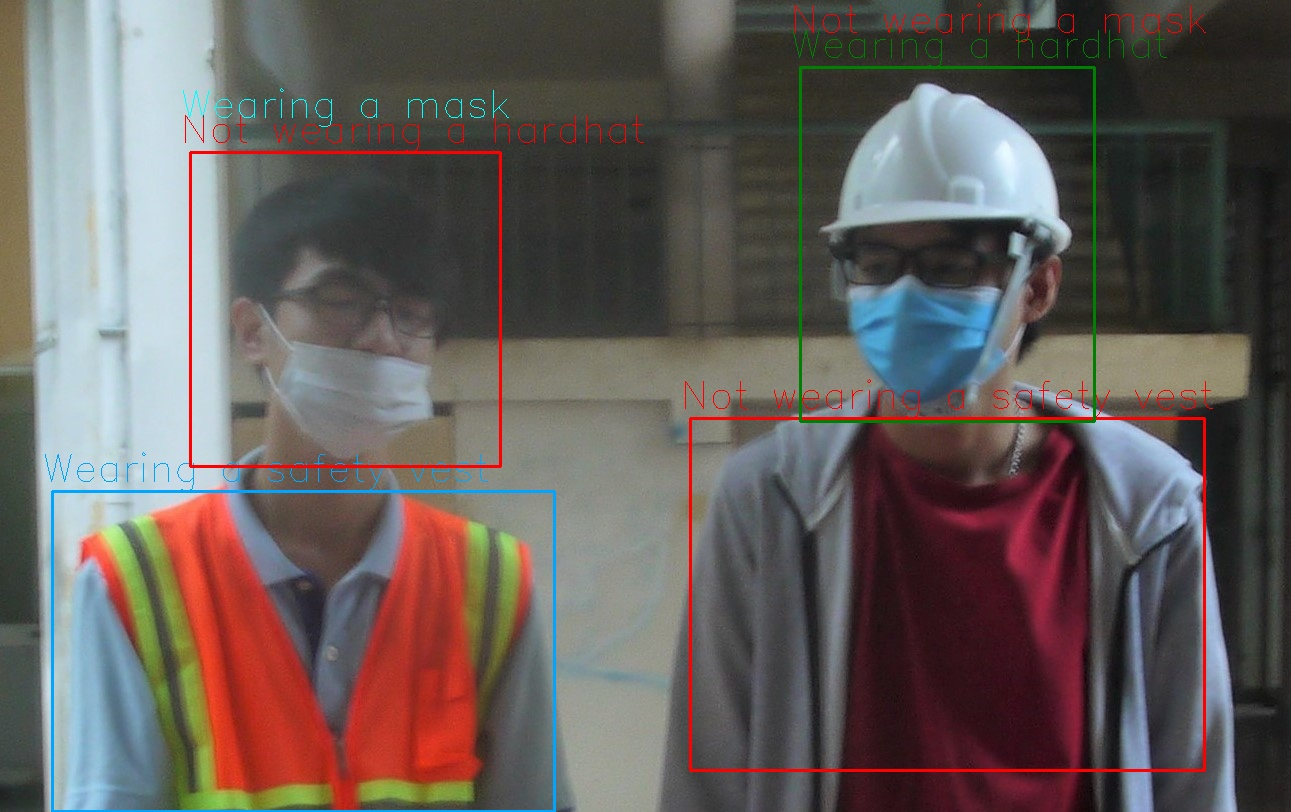
\includegraphics[scale=0.17]{images/bad_mask_nose_pred.jpg}}
  	\caption{The predicted results were not good for the subject (left) wearing a mask that did not cover his nose at a distance of 3m.}
  	\label{fig:bad_mask_nose_pred}
\end{figure}
\begin{figure}[ht]
	\centerline{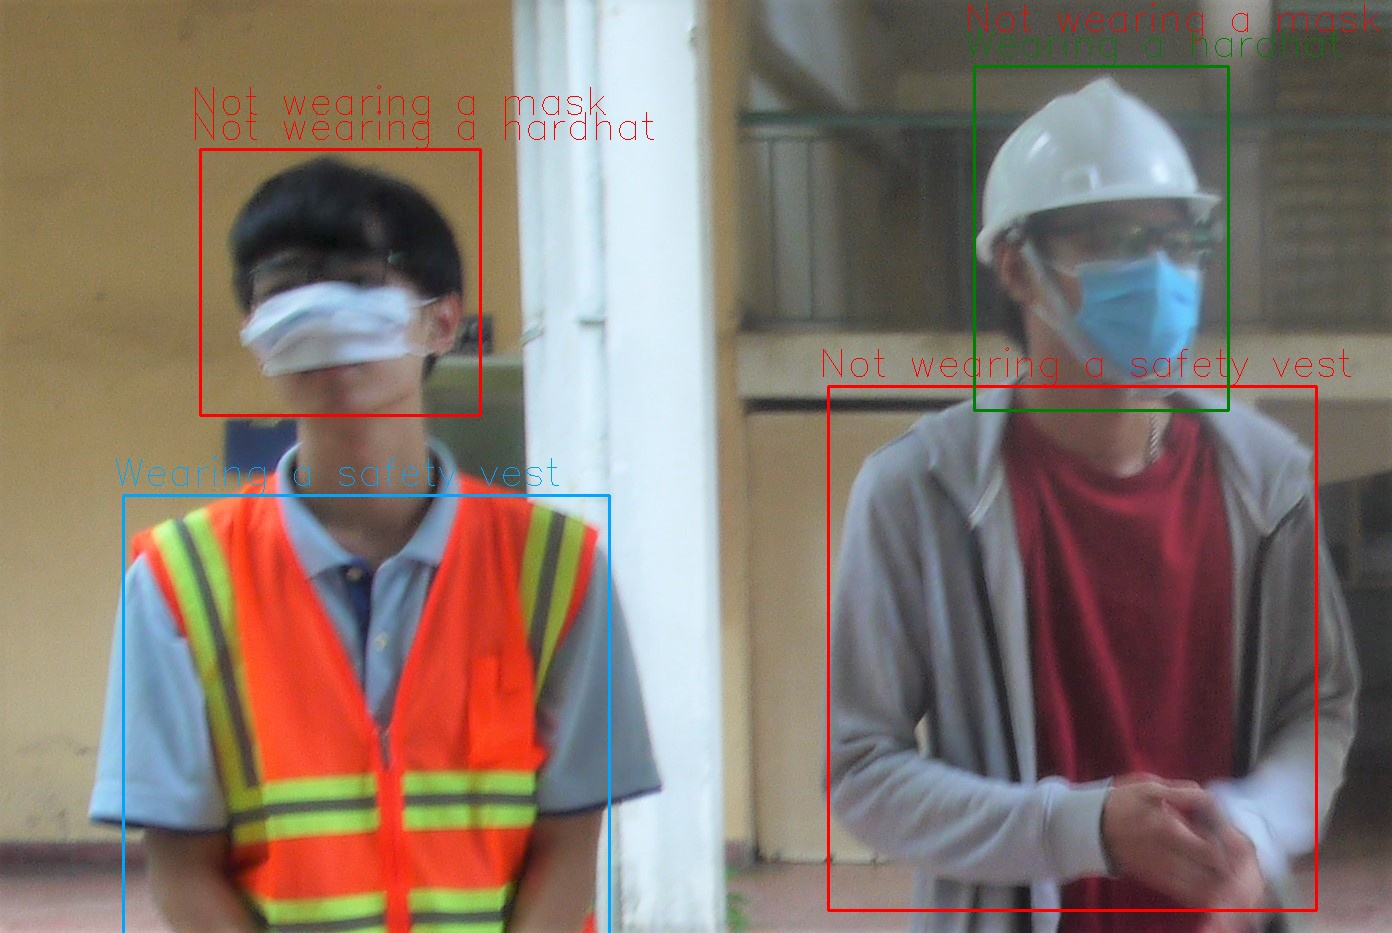
\includegraphics[scale=0.17]{images/bad_mask_mouth_pred.jpg}}
  	\caption{Good predictive results for the subject (left) wearing a mask that does not cover the mouth at a distance of 3m.}
  	\label{fig:bad_mask_mouth_pred}
\end{figure}

\emph{Case 2}: The wearing of the wrong safety vest will be done by putting it only on the person who does not actually wear it or wearing it but does not install it properly as shown in the figure \ref{fig:bad_sv}, which can make the shirt get stuck into active vehicles or machines and causing unfortunate accidents. The predicted results are shown in the figure at a distance of $ 3 $m.
\begin{figure}[ht]
	\centerline{\includegraphics[scale=0.14]{images/bad_sv.jpg}}
  	\caption{The two subjects (leftmost) wear safety vest at a distance of 3m.}
  	\label{fig:bad_sv}
\end{figure}
\emph{Result}: The model can distinguish cases of wearing protective clothing in most cases as shown in the figures \ref{fig:bad_sv_pred_1} and \ref{fig:bad_sv_pred_2}. However, at some angles as shown in the figure \ref{fig:bad_sv_pred_3}, the model could not identify correctly. This may not be a major drawback because when identified in practice, the model will recognize continuously across multiple frames, so that cases of faulty wearing when omitted at this frame will be detected in other frames.
\begin{figure}[ht]
	\centerline{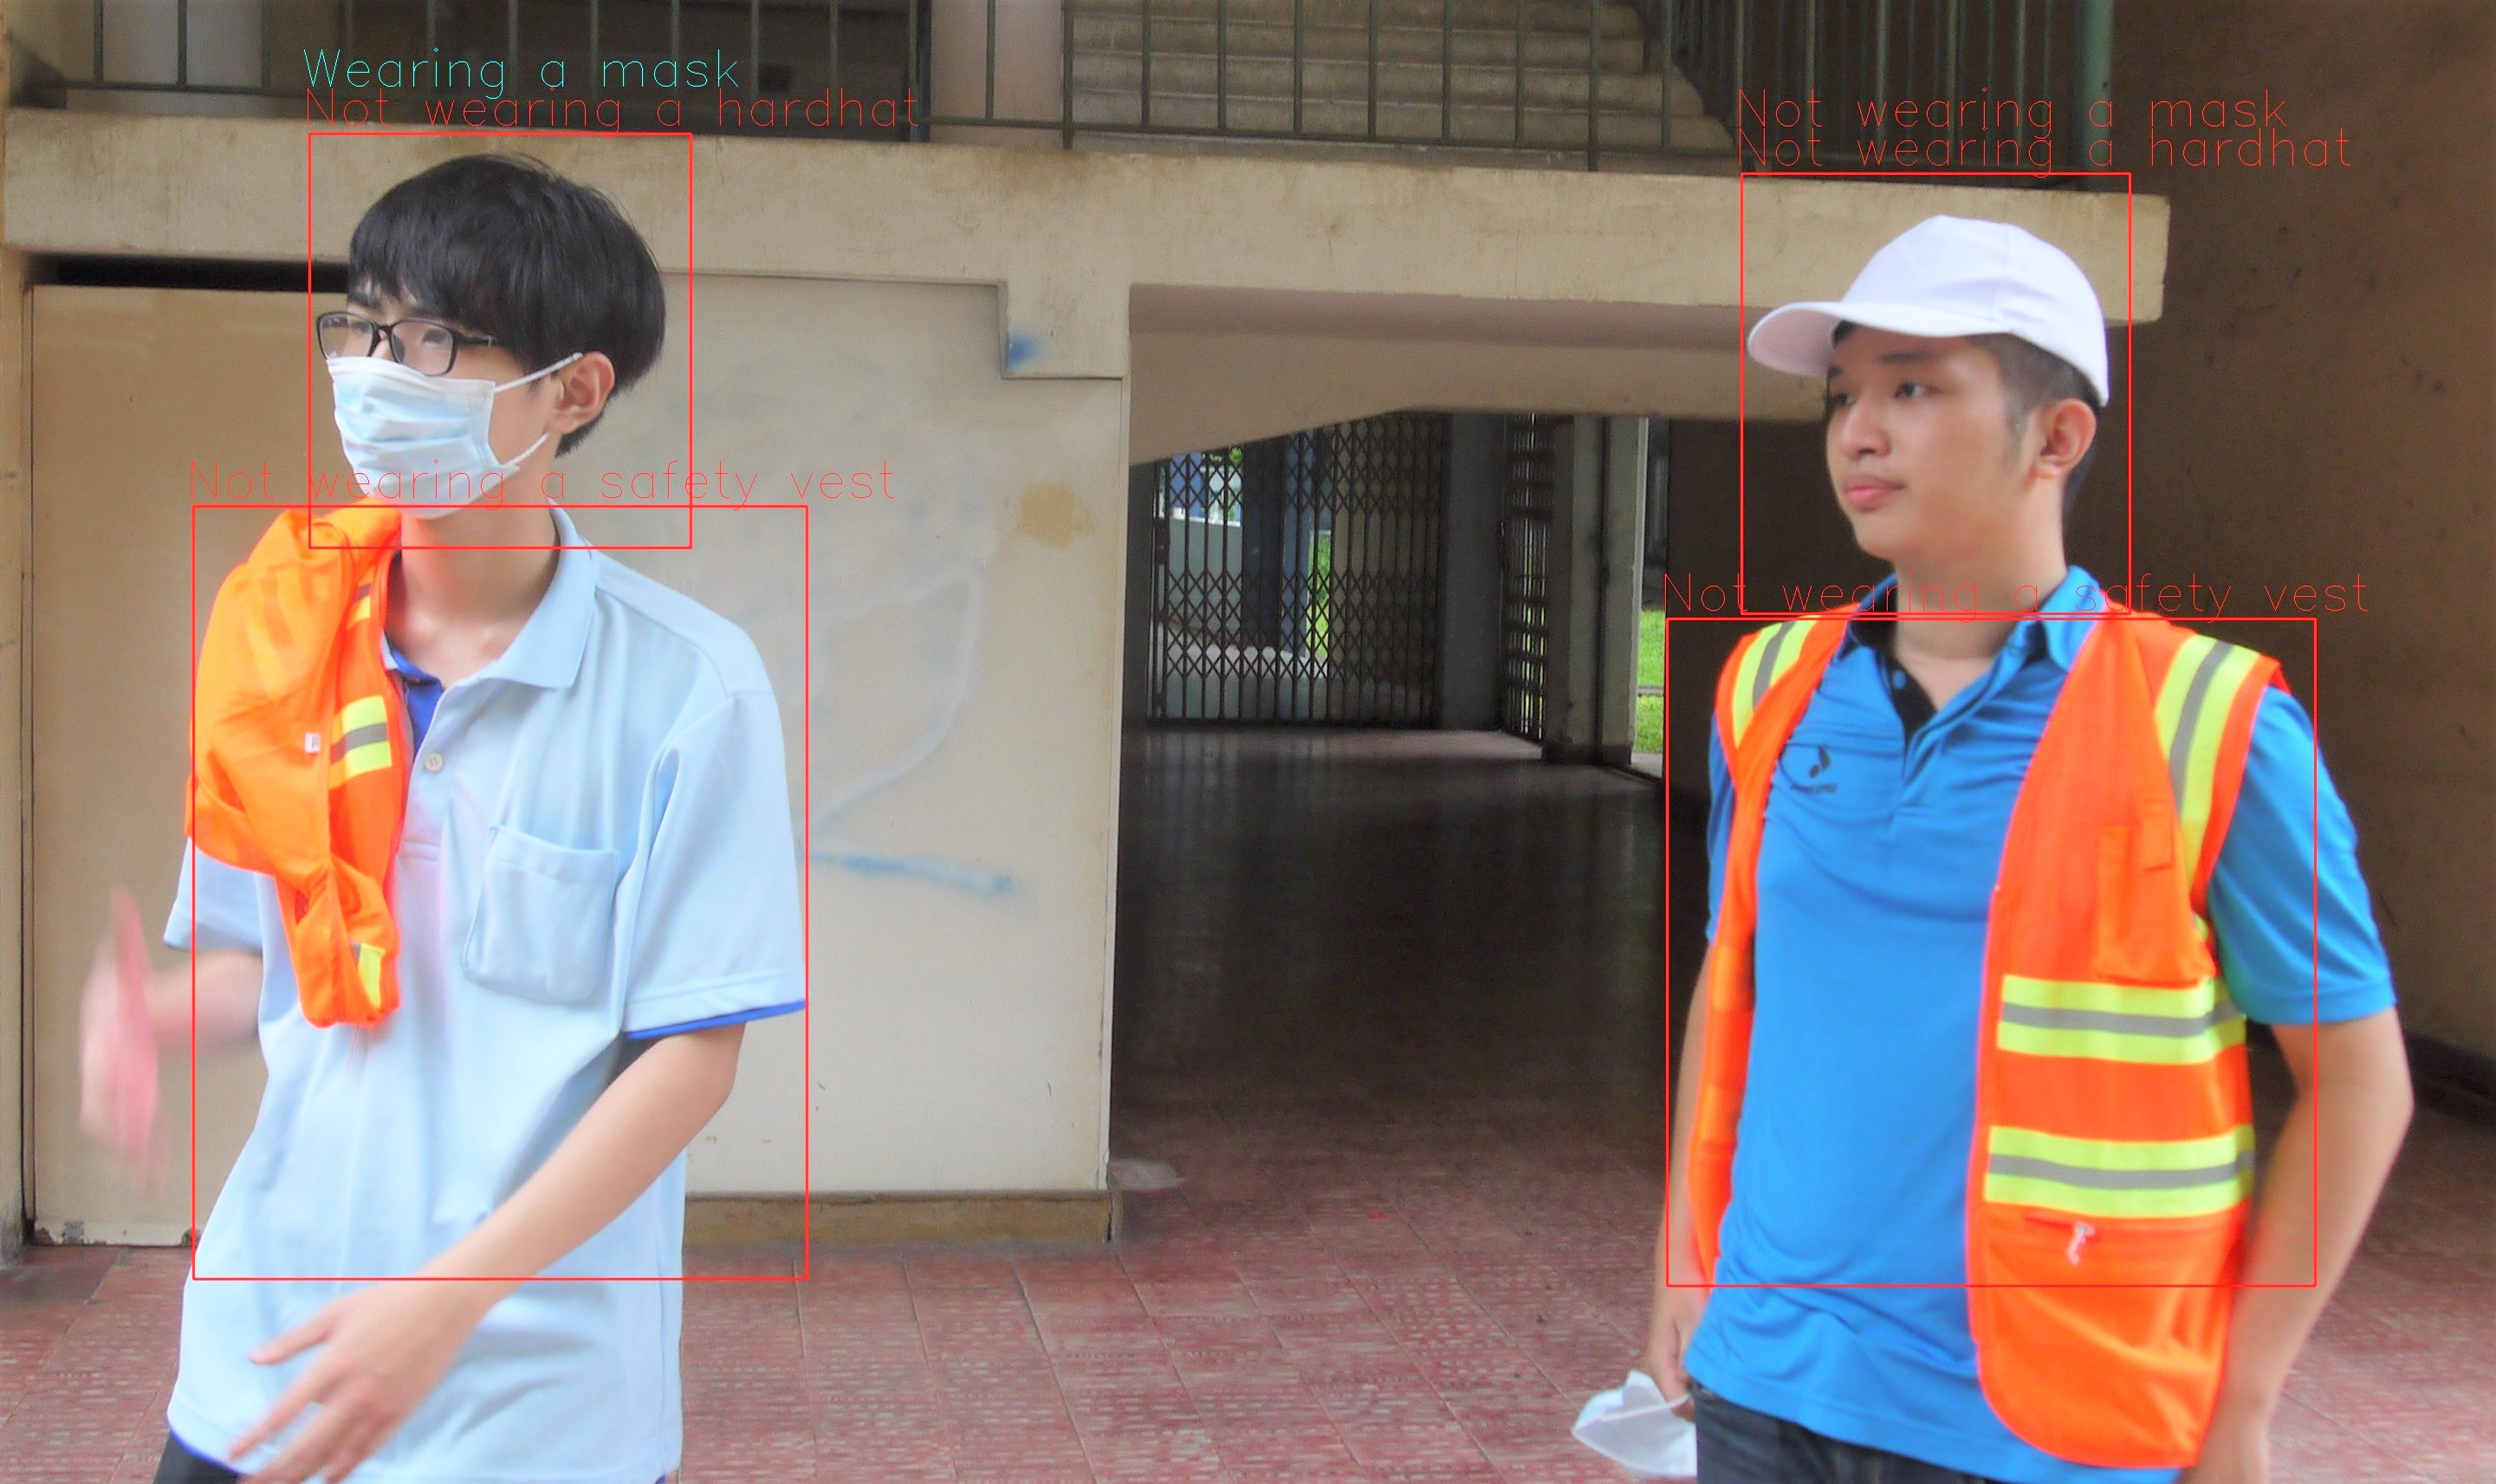
\includegraphics[scale=0.1]{images/bad_sv_predict_2.jpg}}
  	\caption{The good prediction with two subjects wearing the safety vests the wrong way at a distance of 3m.}
  	\label{fig:bad_sv_pred_1}
\end{figure}
\begin{figure}[ht]
	\centerline{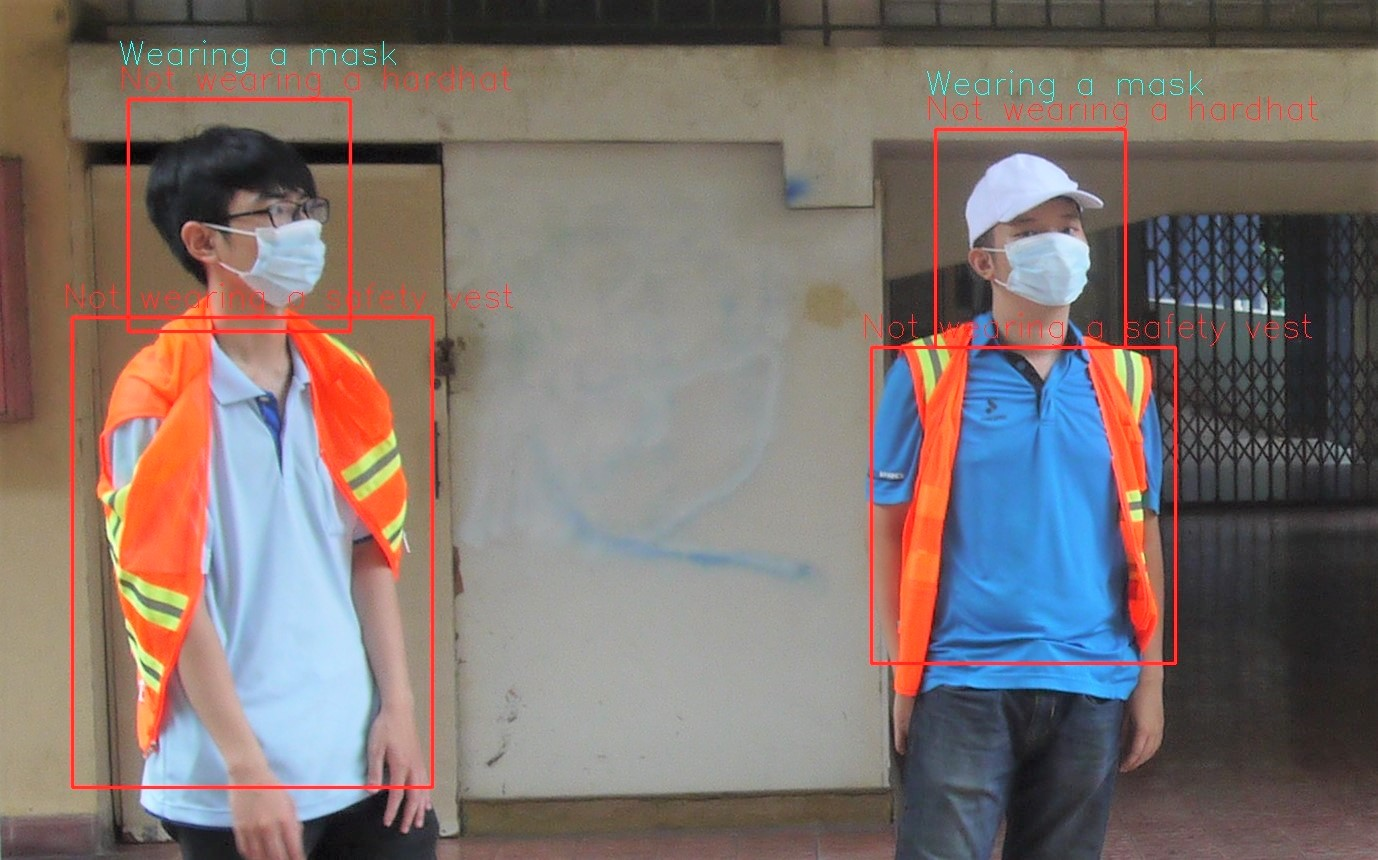
\includegraphics[scale=0.21]{images/bad_sv_predict_3.jpg}}
  	\caption{The good prediction with two subjects wearing the safety vests the wrong way (other camera angles) at a distance of 3m.}
  	\label{fig:bad_sv_pred_2}
\end{figure}
\begin{figure}[ht]
	\centerline{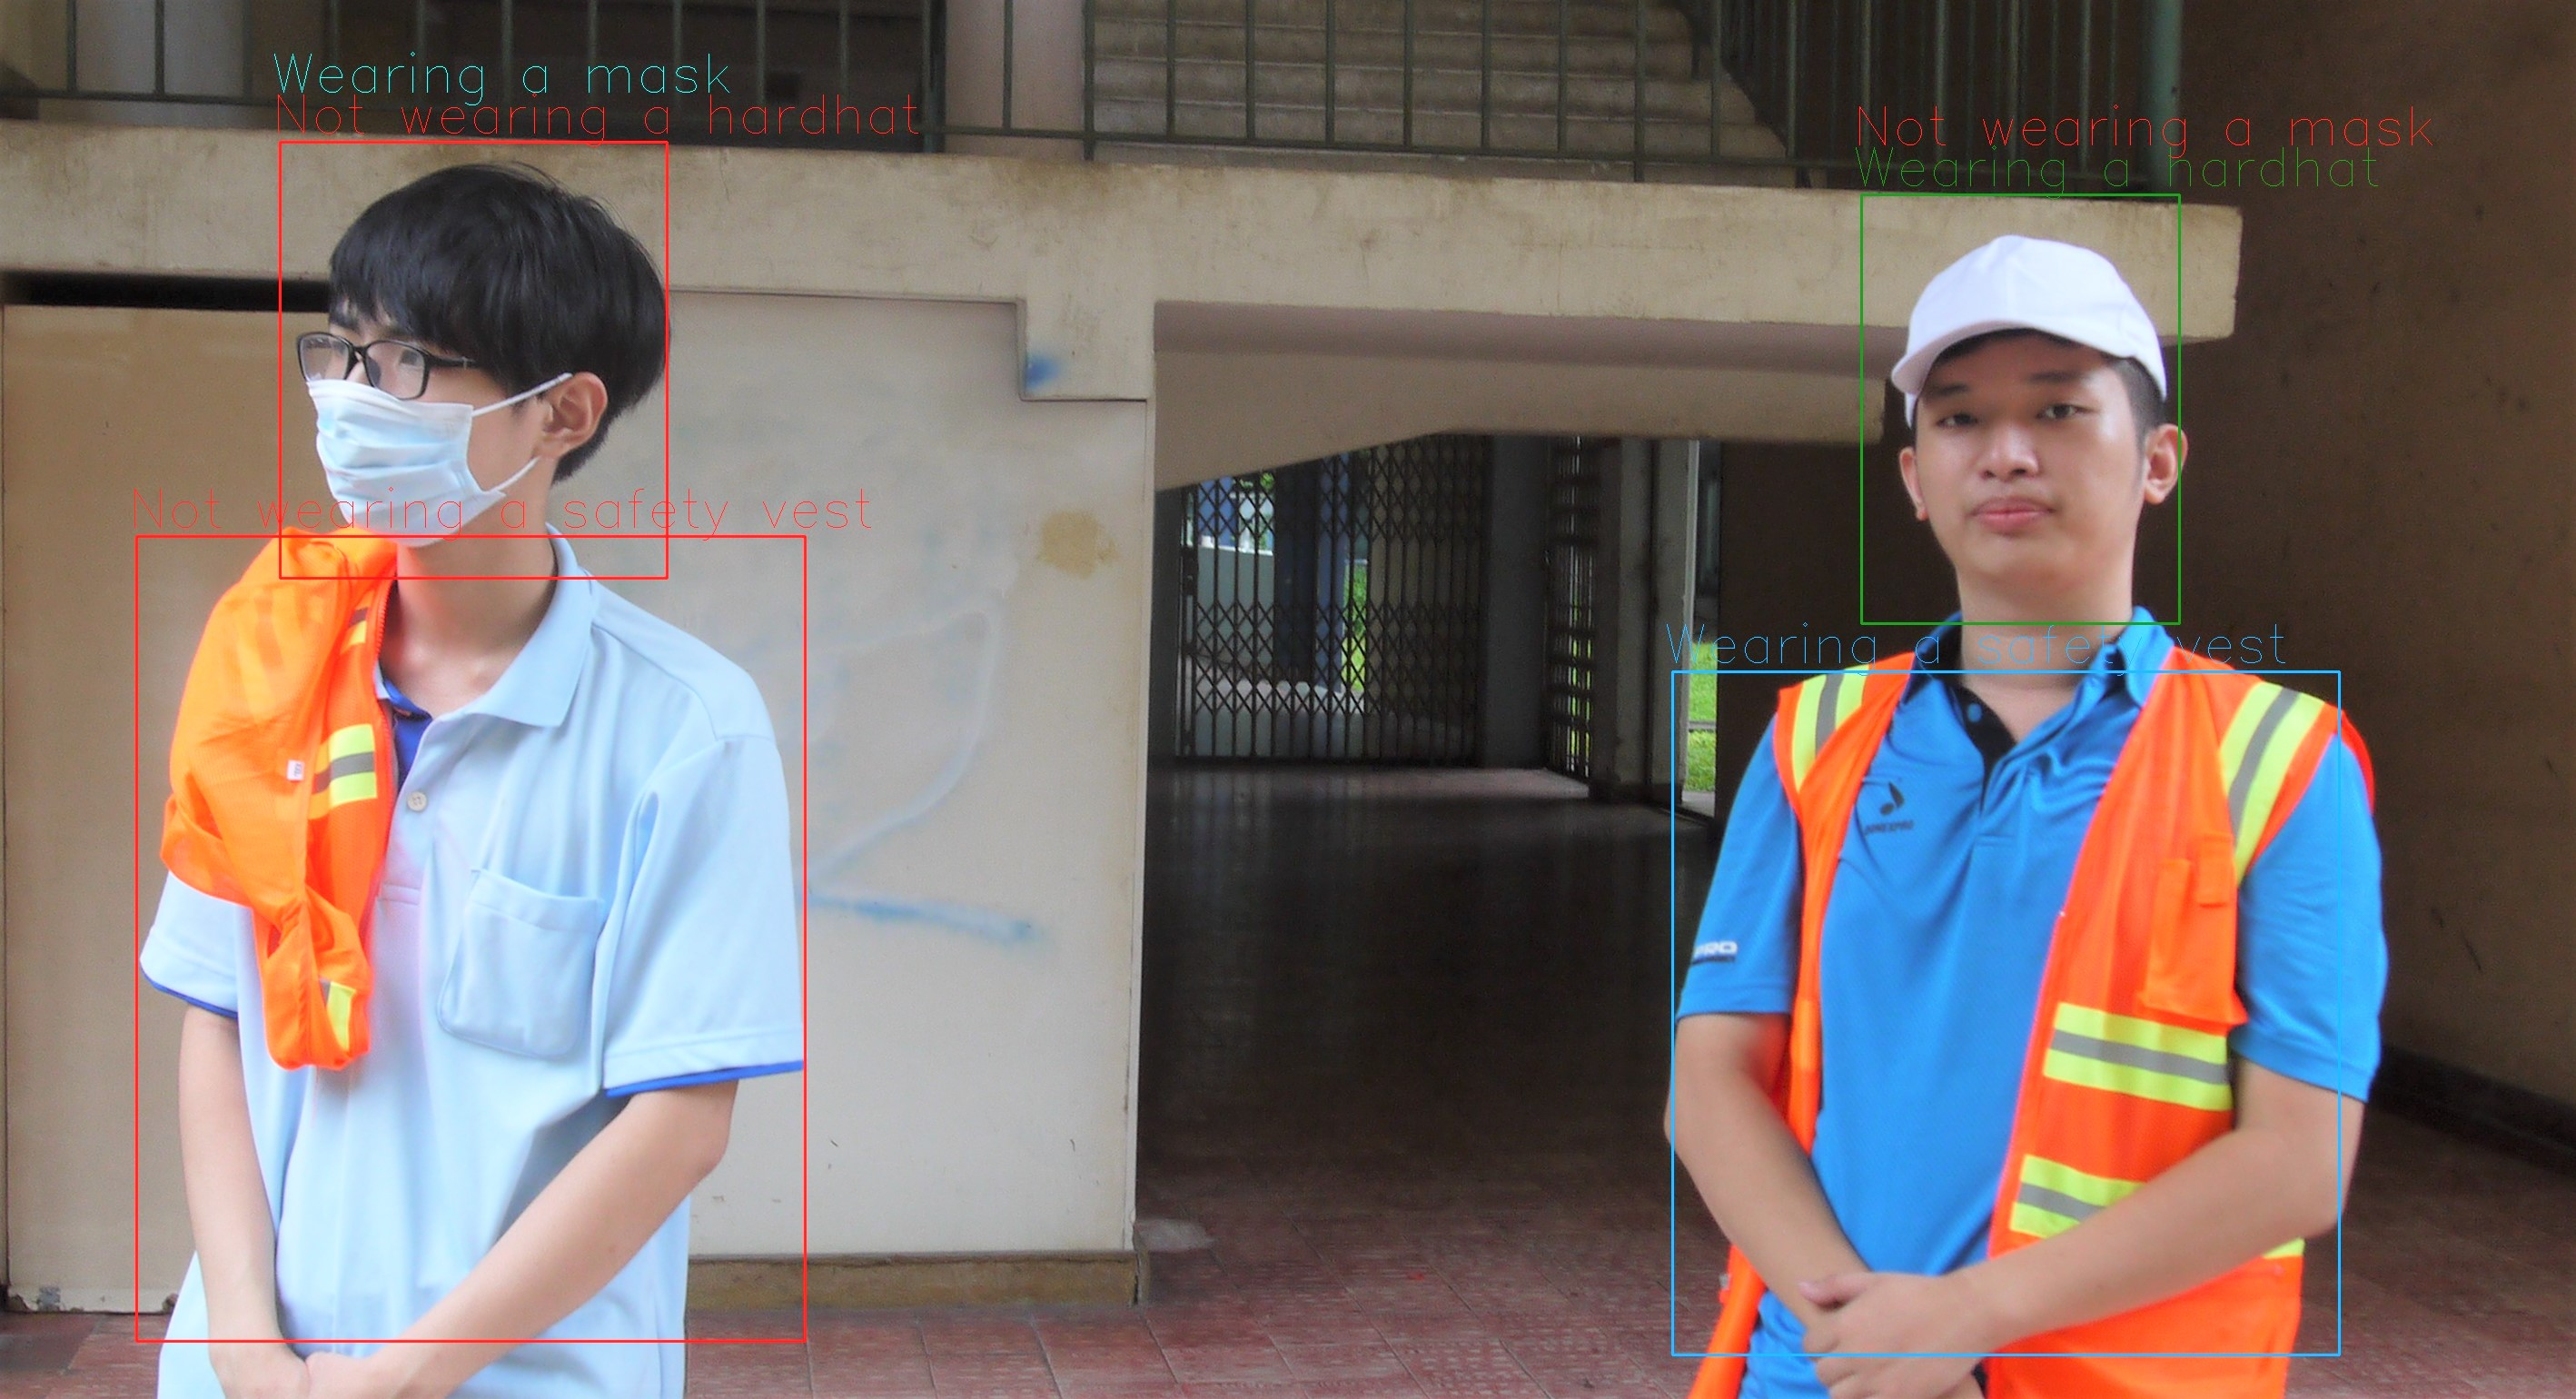
\includegraphics[scale=0.095]{images/bad_sv_predict_4.jpg}}
  	\caption{The bad prediction with two subjects wearing the safety vests the wrong way at a distance of 3m.}
  	\label{fig:bad_sv_pred_3}
\end{figure}

\subsubsection{Testing the recognition ability of the model when the subject is behind obstacles}
In this test, two subjects will be behind an obstacle: the iron door as shown in the image \ref{fig:obstacle}, the model's precision and recall parameters will be calculated based on the predicted result of the model. The photo on the figures is at a distance of $ 3 $ m and $ 6 $ m.
\begin{figure}[ht]
	\centerline{\includegraphics[scale=0.13]{images/obstacle.JPG}}
  	\caption{Two subjects stand behind obstacles at a distance of 3m.}
  	\label{fig:obstacle}
\end{figure}

\emph{Result}: The precision values in figure \ref{fig:3_6_precision} and recall values in figure \ref{fig:3_6_recall} of the model when predicting the subject behind the obstacle are very low at 3m and 6m. This proves that the model cannot be used to identify in cases of obstacles.
\begin{figure}[ht]
	\centerline{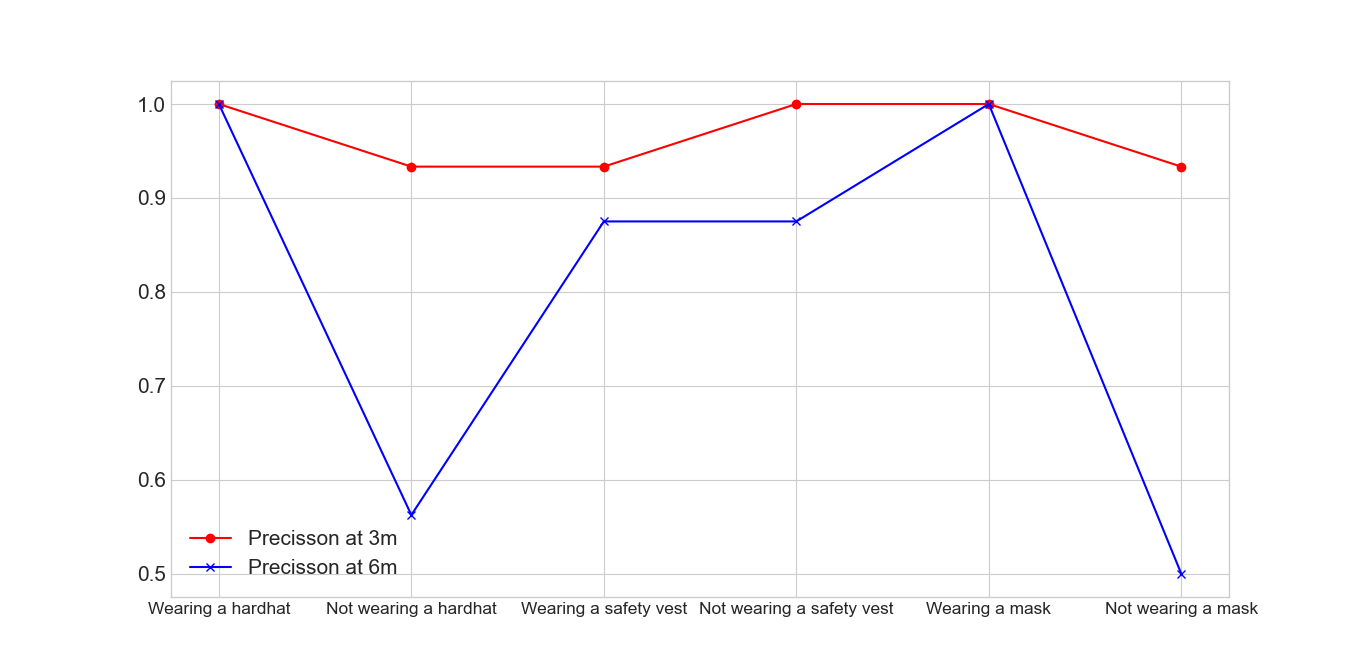
\includegraphics[scale=0.3]{images/3_6_precision.png}}
  	\caption{Precision of classes when subjects are behind obstacles and 3m away from the camera - red and 6m - blue.}
  	\label{fig:3_6_precision}
\end{figure}
\begin{figure}[ht]
	\centerline{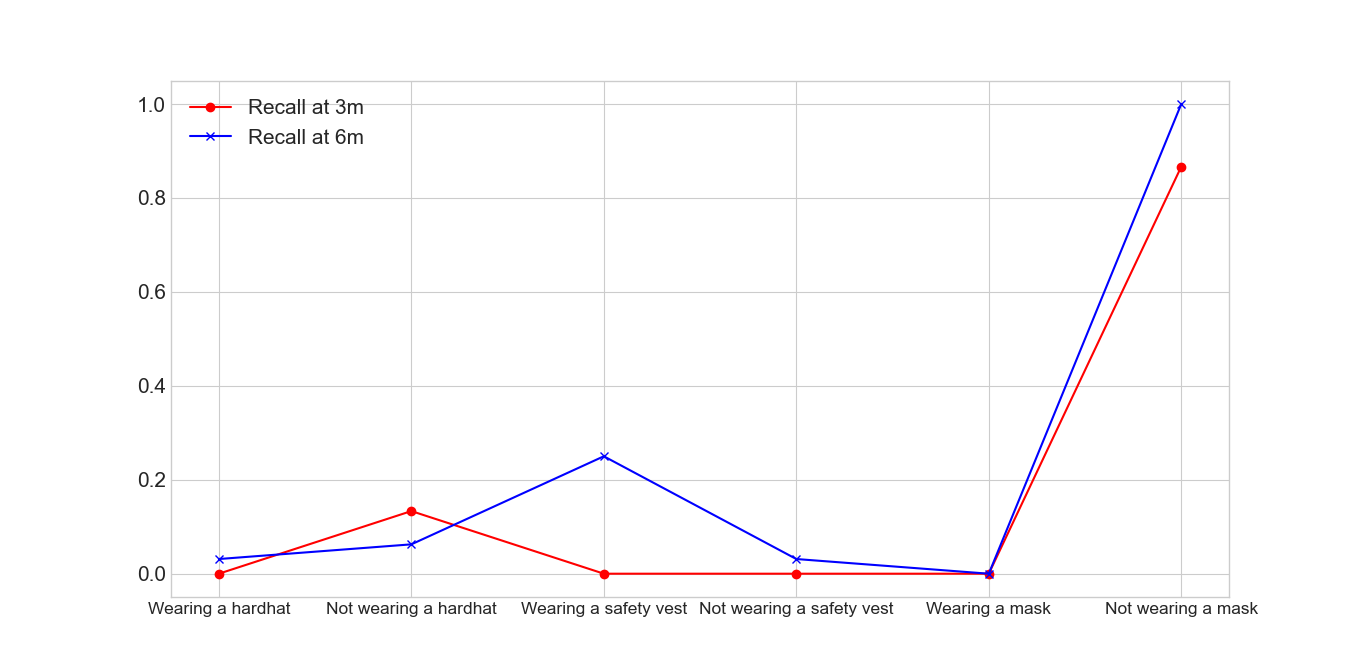
\includegraphics[scale=0.3]{images/3_6_recall.png}}
  	\caption{Recall of classes when subjects are behind obstacles and 3m away from the camera - red and 6m - blue.}
  	\label{fig:3_6_recall}
\end{figure}
\section*{Conclusion}
\subsection{On the model's ability to identify the use of personal protective equipment}
This paper has successfully built a monitoring system for the use of personal protective equipment on the basis of convolutional neural network. The system uses the YOLOv3 model to be trained from the beginning on a custom data set with a total of $ 11586 $ images with different scenes and times to ensure the model is not too familiar with a certain context. After testing the model in practice, the following conclusions can be drawn about the identification of the model:
\begin{itemize}
	\item The model gives good predicting performance with an average accuracy between classes of approximately $ 84 \% $ and sensitivity of approximately $ 86 \% $ at a distance of $ 6 $ m. As the distance increases or decreases, the model's prediction capability starts to decrease.
	\item Models can be used to detect cases of misuse of hard hats, safety vests, or masks. However, the ability to identify the model in these cases is limited and depends heavily on the camera's rotation angle and the position of the subject in the frame.
	\item If there is an obstruction between the subject and the camera that partially obscures the subject, the model cannot be used for identification in these cases.
	\item The processing speed of the model is still slow, the model takes $ 0.712 $ seconds to predict on an image on a computer with Intel Core i5-6300U CPU @ 2.40GHz, 8.00 GB RAM. When performing prediction on the computer's webcam, the model runs at a speed of $ 0.4 $ frame/s.
\end{itemize}

\subsection{Possible improvement}
The issue of ensuring labor safety always receives the attention of the society, improving the supervisory capacity in the areas where it is necessary to ensure the provision of personal protective equipment will help improve the working environmental quality of not only the construction industry but also other high risk industries such as mines, iron fabrication, etc. In order to be truly reliable to be used in real life, the system needs to guaranteed to gives precision over $ 95 \% $. To achieve this goal, several improvements can be applied:
\begin{itemize}
	\item Increase the number of images in the data set with different backgrounds so that the model can learn more special cases.
	\item Use newer convolutional network architectures like YOLOv4 to increase accuracy.
	\item Building hardware systems optimized for convolutional neural network to run the model in real time.
\end{itemize}

\bibliography{references}\newpage
\bibliographystyle{ieeetr}
\end{document}
